\documentclass[12pt, letterpaper]{article}
\usepackage[utf8]{inputenc}
\usepackage[pdftex]{graphicx}
\usepackage{xspace}
\usepackage[stable]{footmisc}
\usepackage{hyperref}
\usepackage{fullpage}
\usepackage{subcaption}
\usepackage{placeins}
\hypersetup{
    colorlinks=true,
    linkcolor=blue,
    filecolor=magenta,      
    urlcolor=cyan,
}
\graphicspath{ {/home/tobiasjenegger/Documents/summary/} }
\title{Radius/Momentum Calculation for S444 Experiment February 2020 - Overview}
\author{Tobias Jenegger}
\date{}
\begin{document}
\begin{titlepage}
\maketitle
\end{titlepage}
\subsection{The Setup}
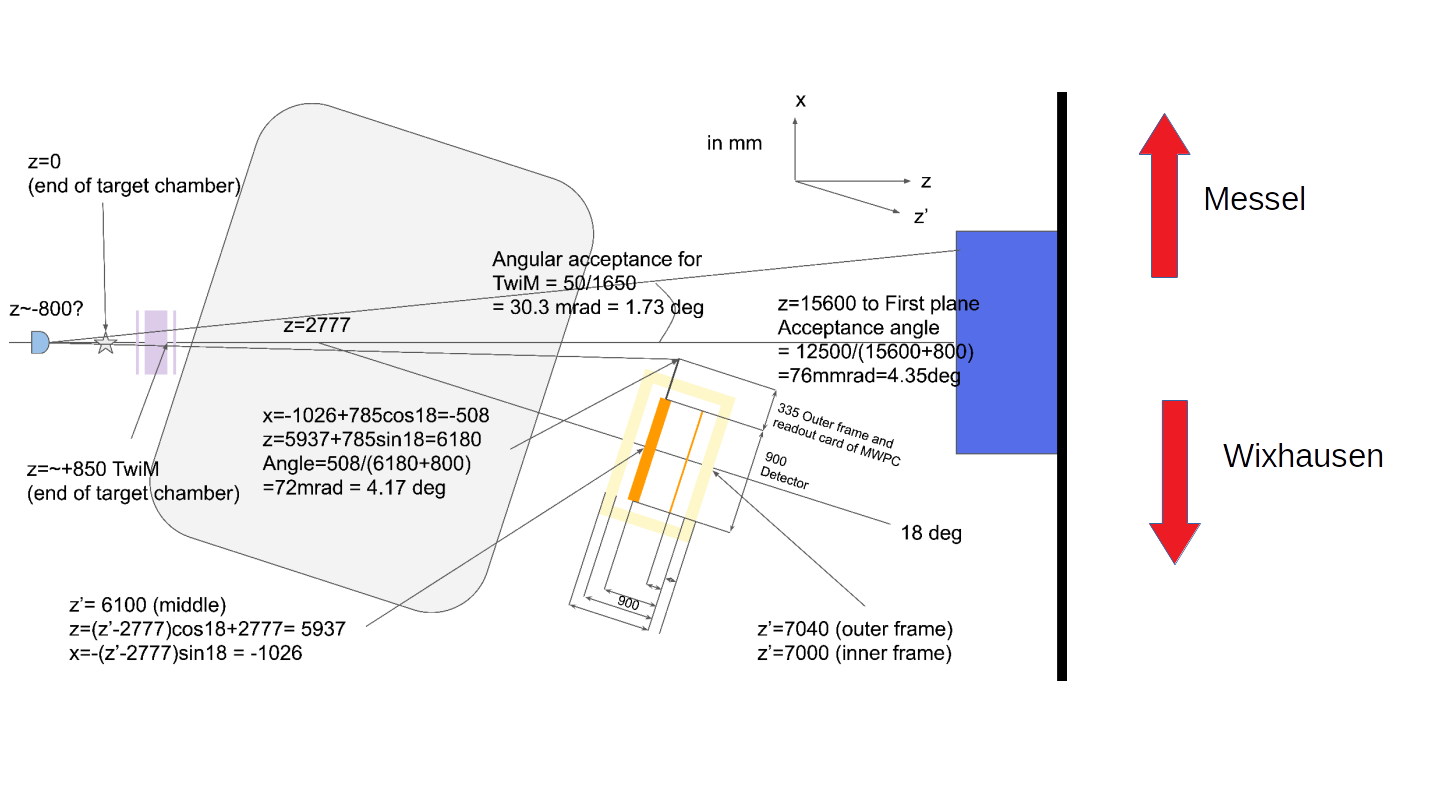
\includegraphics[width=1.0\textwidth]{mes_wixh.png}
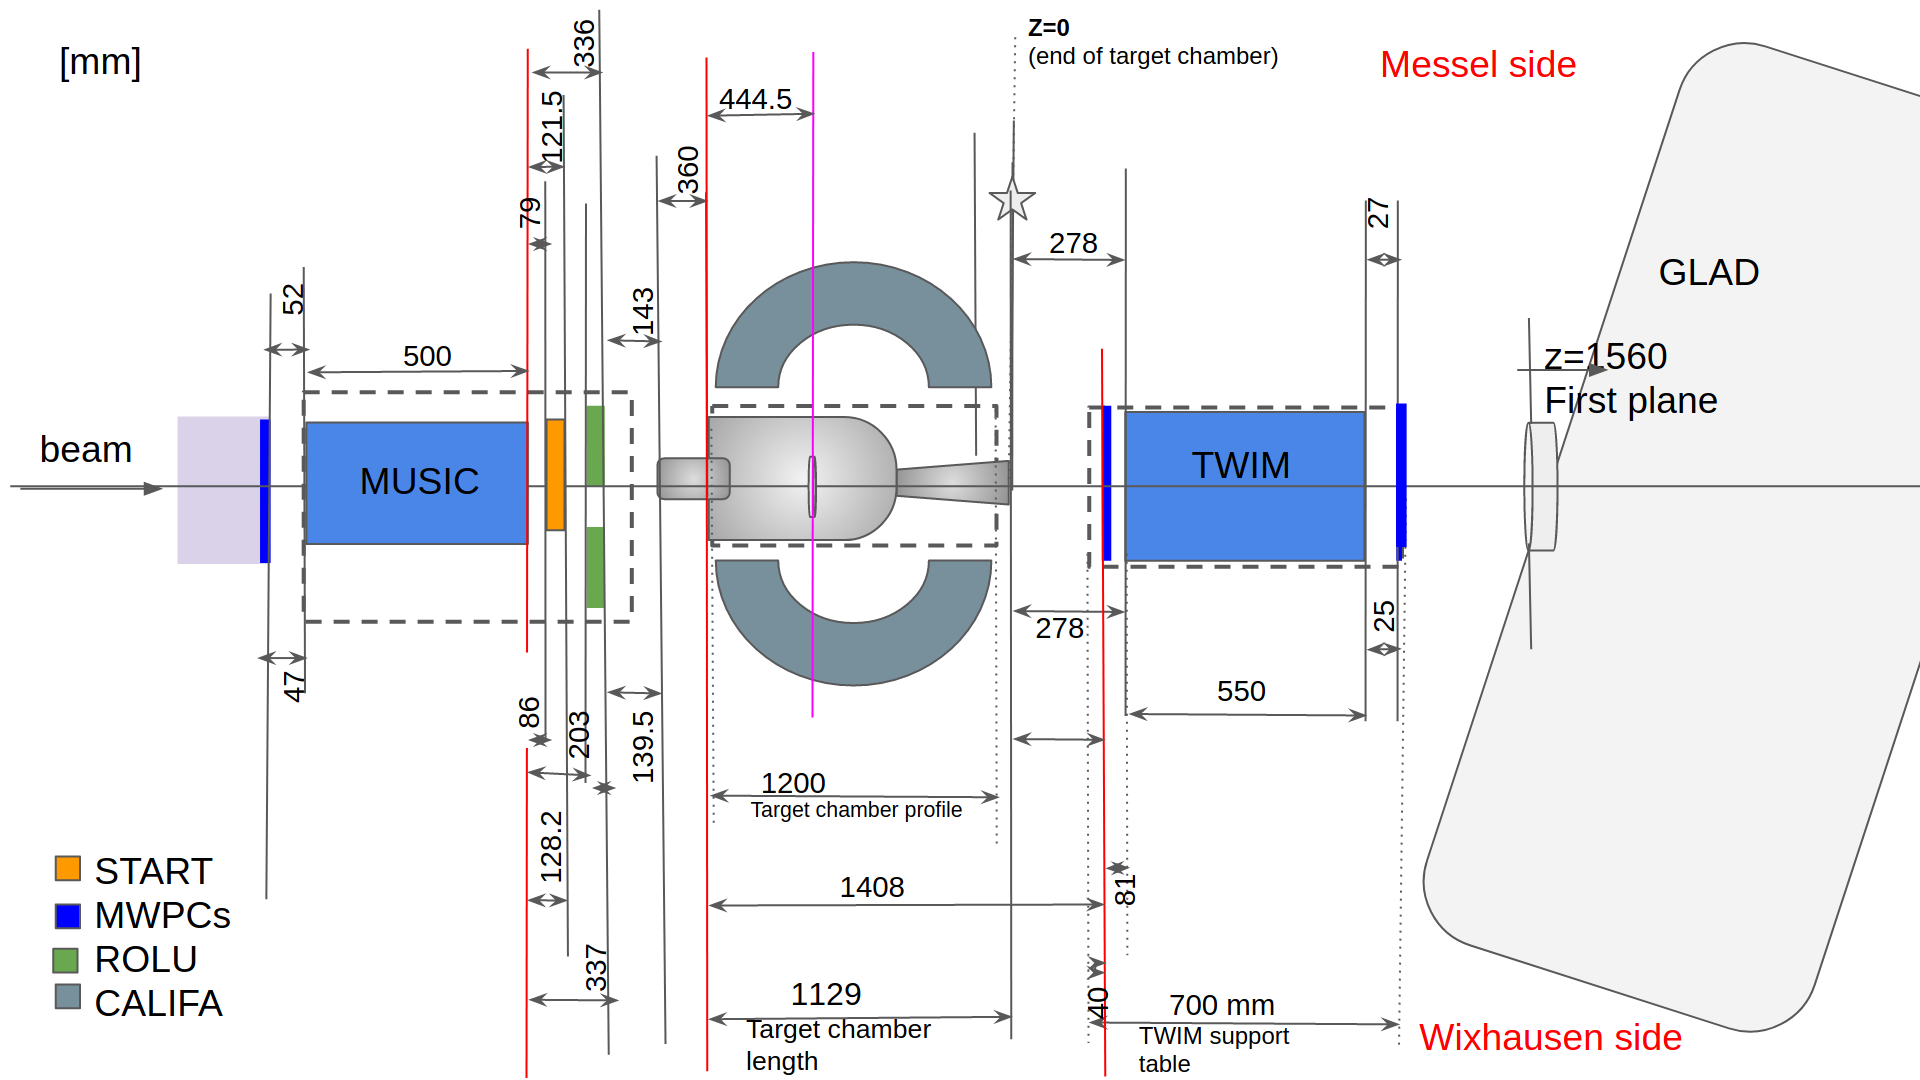
\includegraphics[width=1.0\textwidth]{SETUP_around_Target.png}
\section{Geometry and relative position of the detectors in the beam direction}
Here, the positions are given for the s444 and s467 experiments\\
\\
z position of the MWPC0: \hspace{10mm} zMW0 = -2520 mm\\
z position of the target: \hspace{10mm} zT = -684.5 mm\\
z position of the MWPC1 in front of the Twin-MUSIC:  \hspace{10mm}   zM1 = 279 mm \\
z position of the middle of the Twin-MUSIC:  \hspace{10mm}  zTwin = 553 mm\\
z position of the MWPC2 after the Twin-MUSIC:  \hspace{10mm}   zM2 = 854 mm\\
$\alpha$ tilted angle of GLAD (14 degrees):   \hspace{10mm} = 0.244 rad\\
effective length of GLAD:  \hspace{10mm}   L\textunderscore eff = 2067 mm\\
z middle of GLAD  \hspace{10mm}  zGm = 2577mm\\
horizontal of the central path (18 degree) \hspace{10mm}   $\theta$\textunderscore out0 = pi/10 rad\\
z position of the MWPC3 after GLAD   \hspace{10mm}  zM3 = 5937 mm\\
z position of the ToFwall          \hspace{10mm}     zToFW = 6660.2 mm\\
\\
Correspondence between the GLAD current and the magnetic field:  I = 3584 A, B = 2.2 T \\
\\
Positions of the TOFWPads:\\
1 $\Rightarrow$ Messel\\
27$\Rightarrow$ Wixhausen \\

\section{RUNS used for calibration = SWEEP RUNS without target}

\begin{center}
	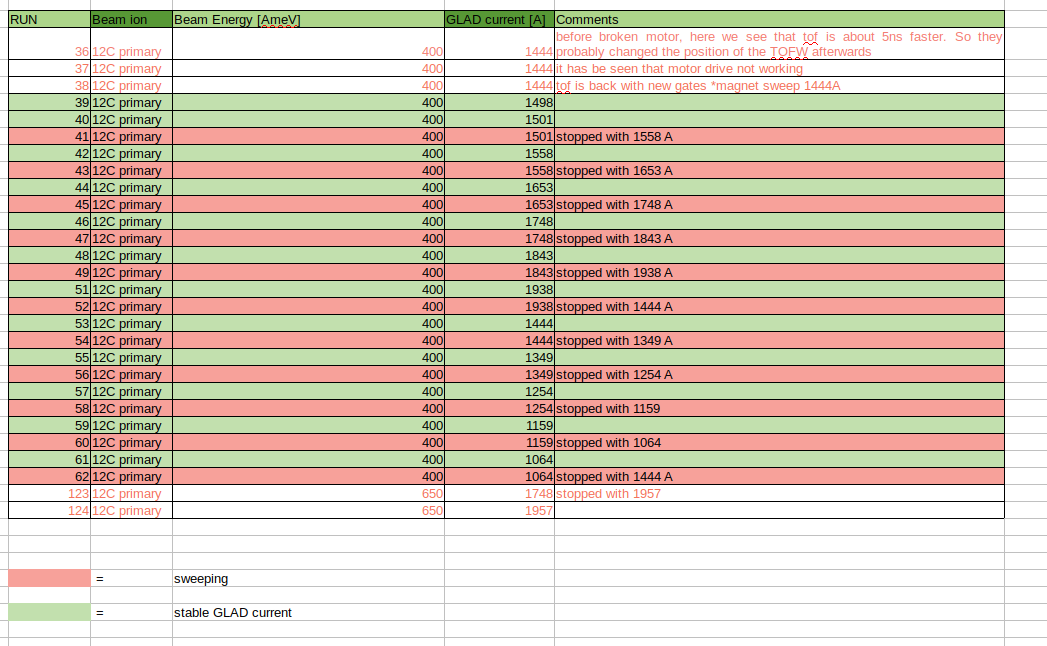
\includegraphics[width=1.0\textwidth]{runs_screenshot.png}
\end{center}

\subsubsection{Other RUNS used for various checks:}
RUN 70: 2 cm C target\\
RUN 80: 10.86 mm C target\\
RUN 81: 24.53 mm CH2 target\\
RUN 67: 24 mm CH2 target \\
RUN 68: 1 cm C target \\
RUN 79: 12.29 mm CH2 target\\
RUN 75: 21.98mm C target\\
\\

\section{Methods for flightpath reconstruction in the (x,z) plane}
\subsection{The "Kickplane" method}
\subsubsection{From MW0 to the entrance of GLAD, the ion is following a straight line}\label{sssec:num1}
\begin{center}
	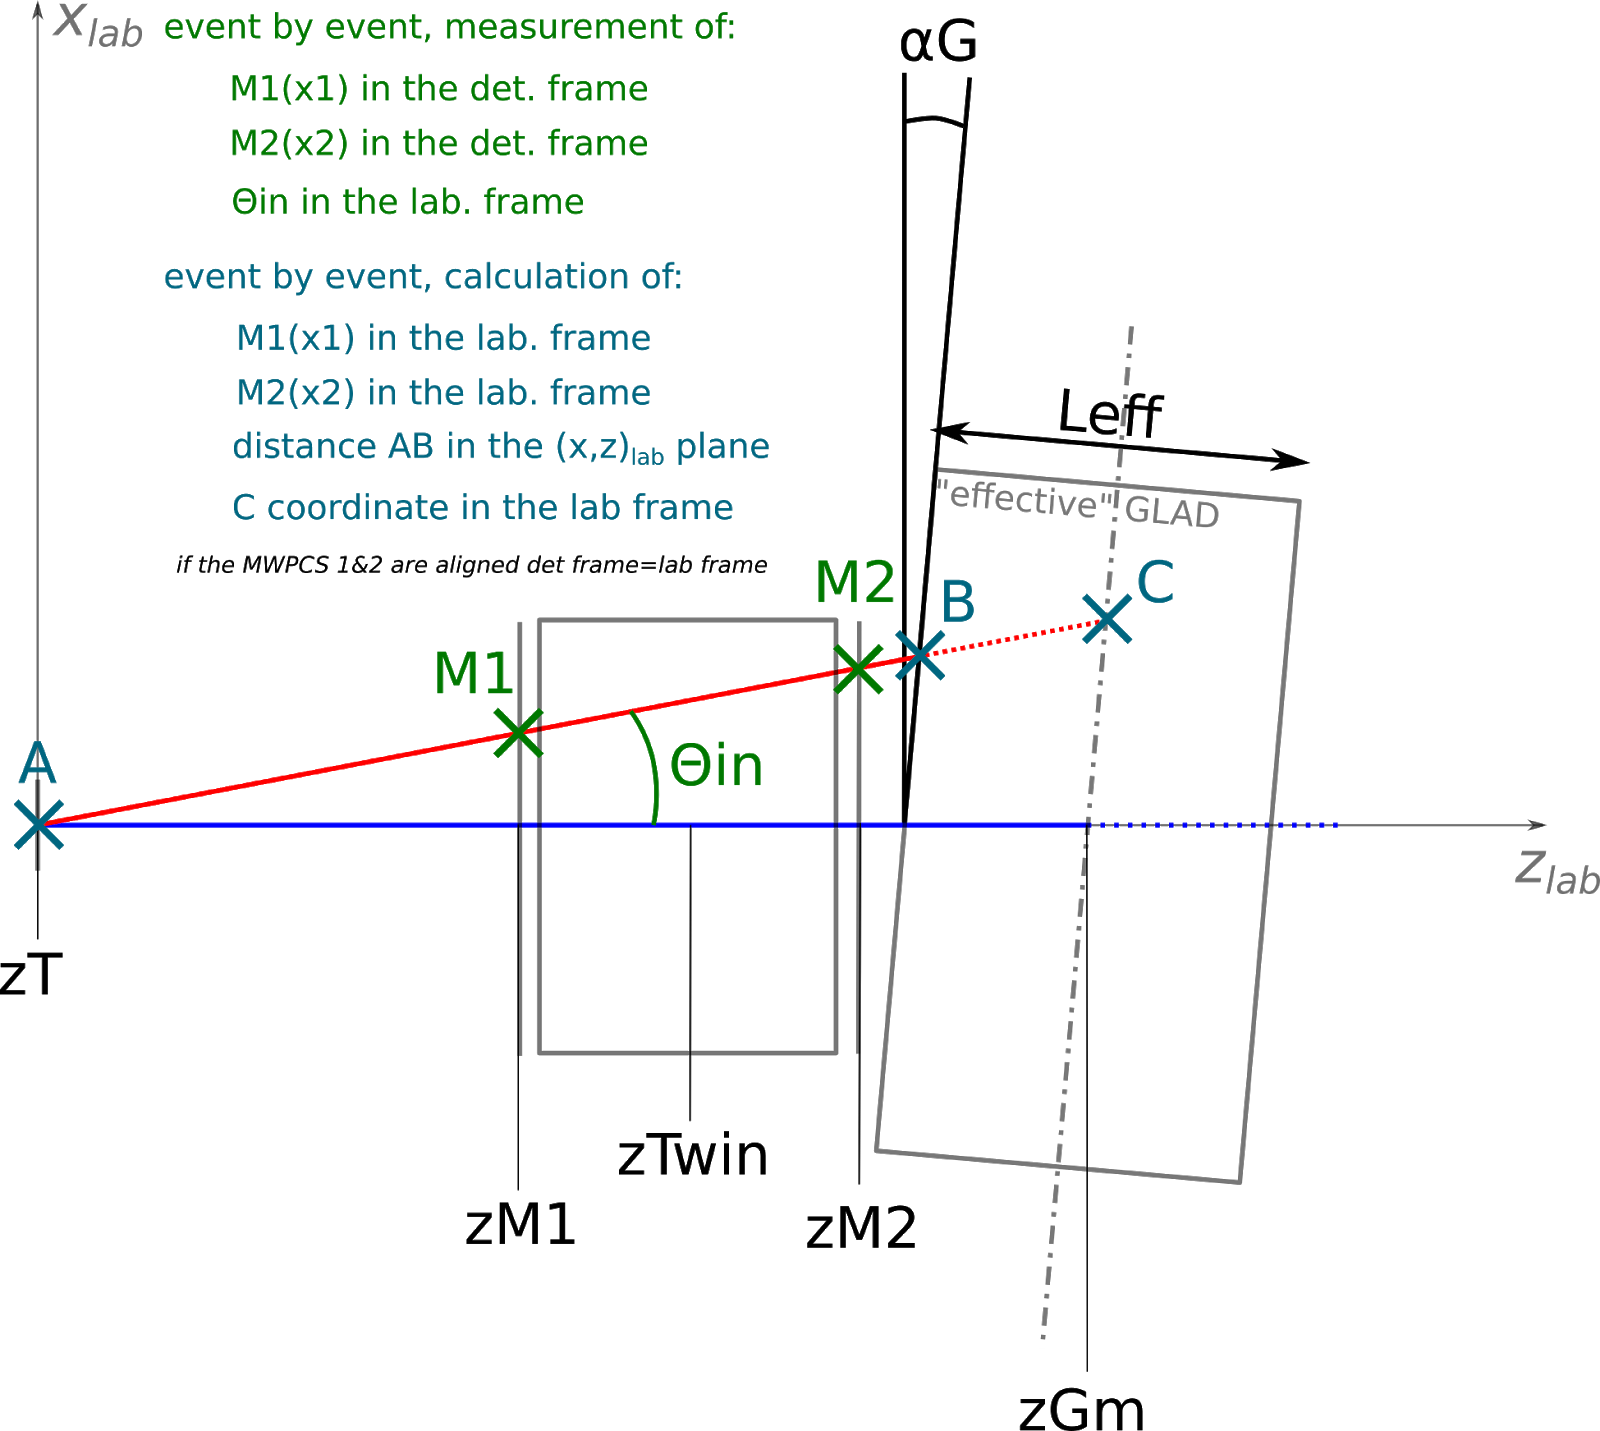
\includegraphics[width=1.0\textwidth]{tracking_upstreamGLAD.png}
\end{center}
\textbf{The straight line trajectory from MW0 to  entrance before glad is defined by:}\\
\textbf{$\Rightarrow$ one absolute value before GLAD}\\
absolute = calibrated position in mm in the laboratory frame\\
To get the position, use the position given by one MWPCs (1 or 2)\\
\\
\textbf{$\Rightarrow$ the theta angle (theta\textunderscore in) before GLAD}\\
Angle obtained from comining MWPC1 and MWPC2\\
(to get higher precision the drift time in TWIM MUSIC could be used)\\
\subsubsection{From entrance to the exit of GLAD, the effective trajectory is circular}
\begin{center}
	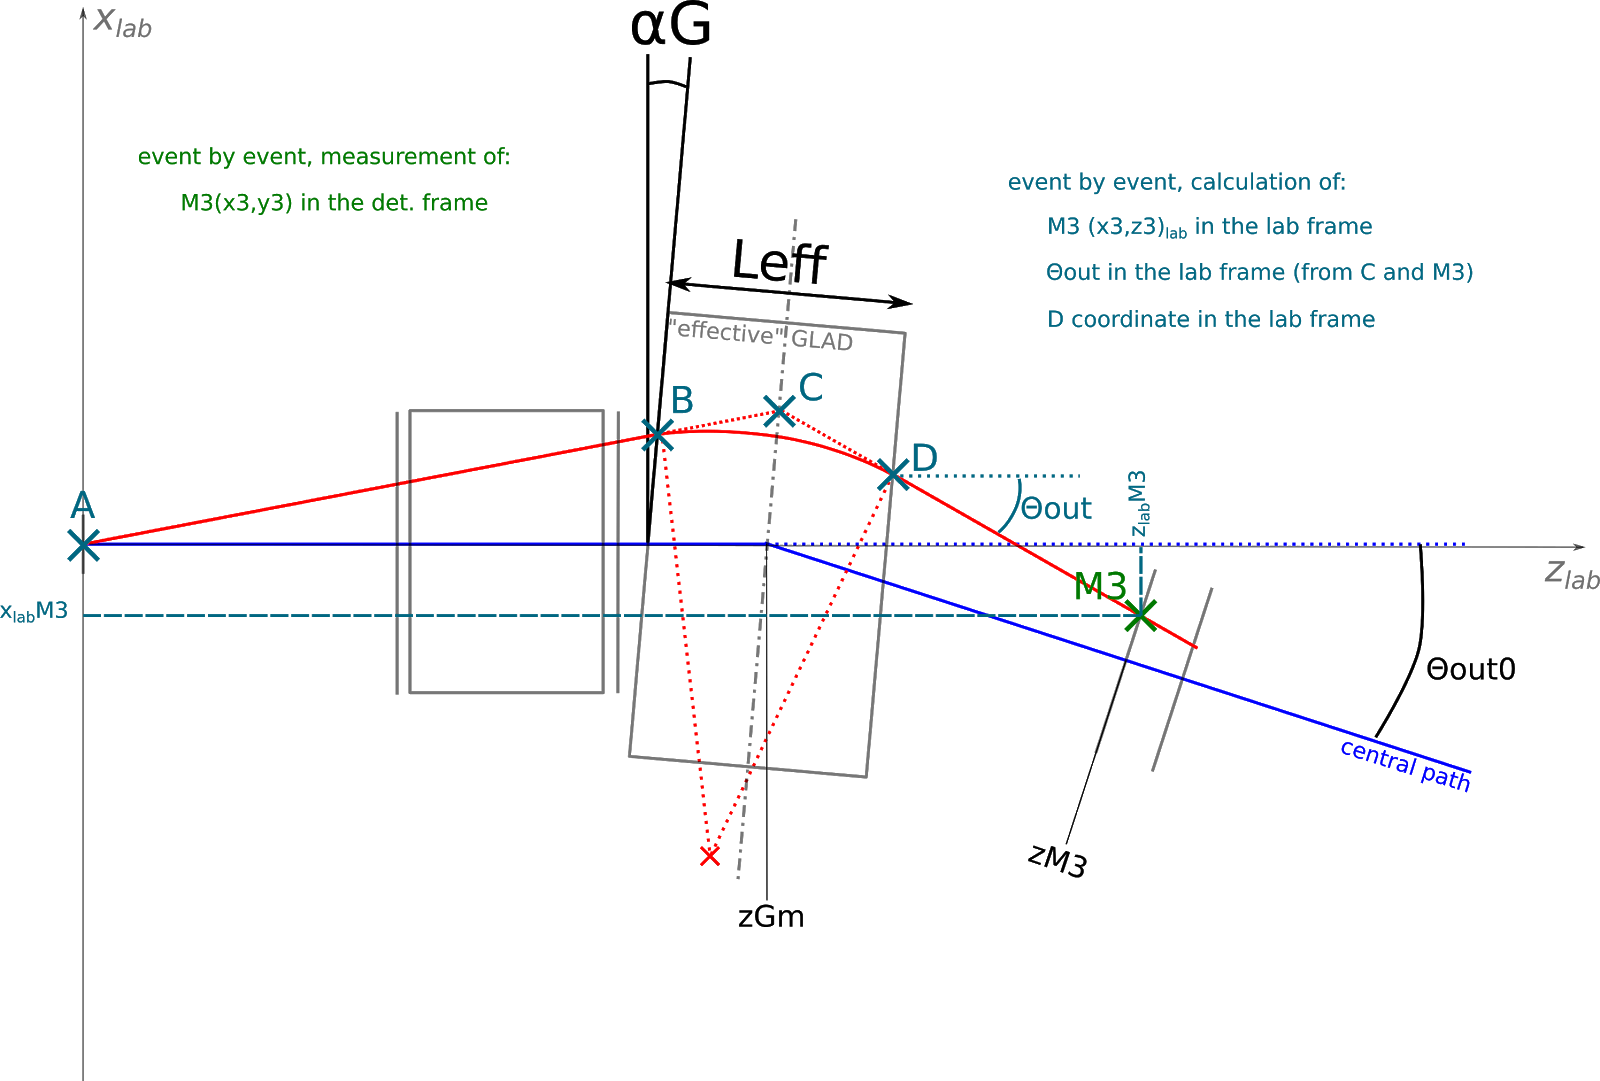
\includegraphics[width=1.0\textwidth]{tracking_GLAD.png}
\end{center}
\textbf{The circular trajectory is defined by:\\
$\Rightarrow$ one absolute position before GLAD B and angle theta\textunderscore in (see: \ref{sssec:num1})\\
$\Rightarrow$ one absolute position at MWPC3}\\
\\
From this information the angle theta\textunderscore out is constructed in follwing steps:\\
\begin{enumerate}
	\item Extend the line of flight of the ion before the GLAD.
	\item The point of intersection with the "kickplane" (symmetry axis line of GLAD magnet) is the kickpoint C.
	\item Draw a straight line between C and the absolute position at MWPC3 = M3.
	 \item theta\textunderscore out is the positive angle between the z-beam direction and the line between C and M3.
\end{enumerate}
The curvature radius $\rho$ is given by\footnote{for consistency checks the $\cos(\delta)$ term can be omitted, as it plays a minor role}:\\
$\rho$ = $\frac{\textrm{L\textunderscore eff}}{2\cdot\sin\left(\frac{theta\textunderscore in}{2} +\frac{theta\textunderscore out}{2}\right)\cdot\cos(\delta)}$\\
\\
With $\delta$: \\
$\delta = \arctan\left( \Bigg| \frac{\frac{cos(theta\textunderscore out)-\cos(theta\textunderscore in)}{\sin(theta\textunderscore out)+\sin(theta\textunderscore in)}+\tan(\alpha)}{1-\frac{cos(theta\textunderscore out)-\cos(theta\textunderscore in)}{\sin(theta\textunderscore out)+\sin(theta\textunderscore in)}\cdot\tan(\alpha)}\Bigg| \right)$ \\
The full derivation can be found in the appendix.\\
\\
The circular trajectory is then given by:\\
$\omega = 2*\Bigg|\arcsin\Big[\frac{BD}{2\cdot\rho}\Big] \Bigg|$\\
\\
with BD = length of the BD segment\\
\subsubsection{After GLAD up to the TOFW, the trajectory is a straight line}
\begin{center}
	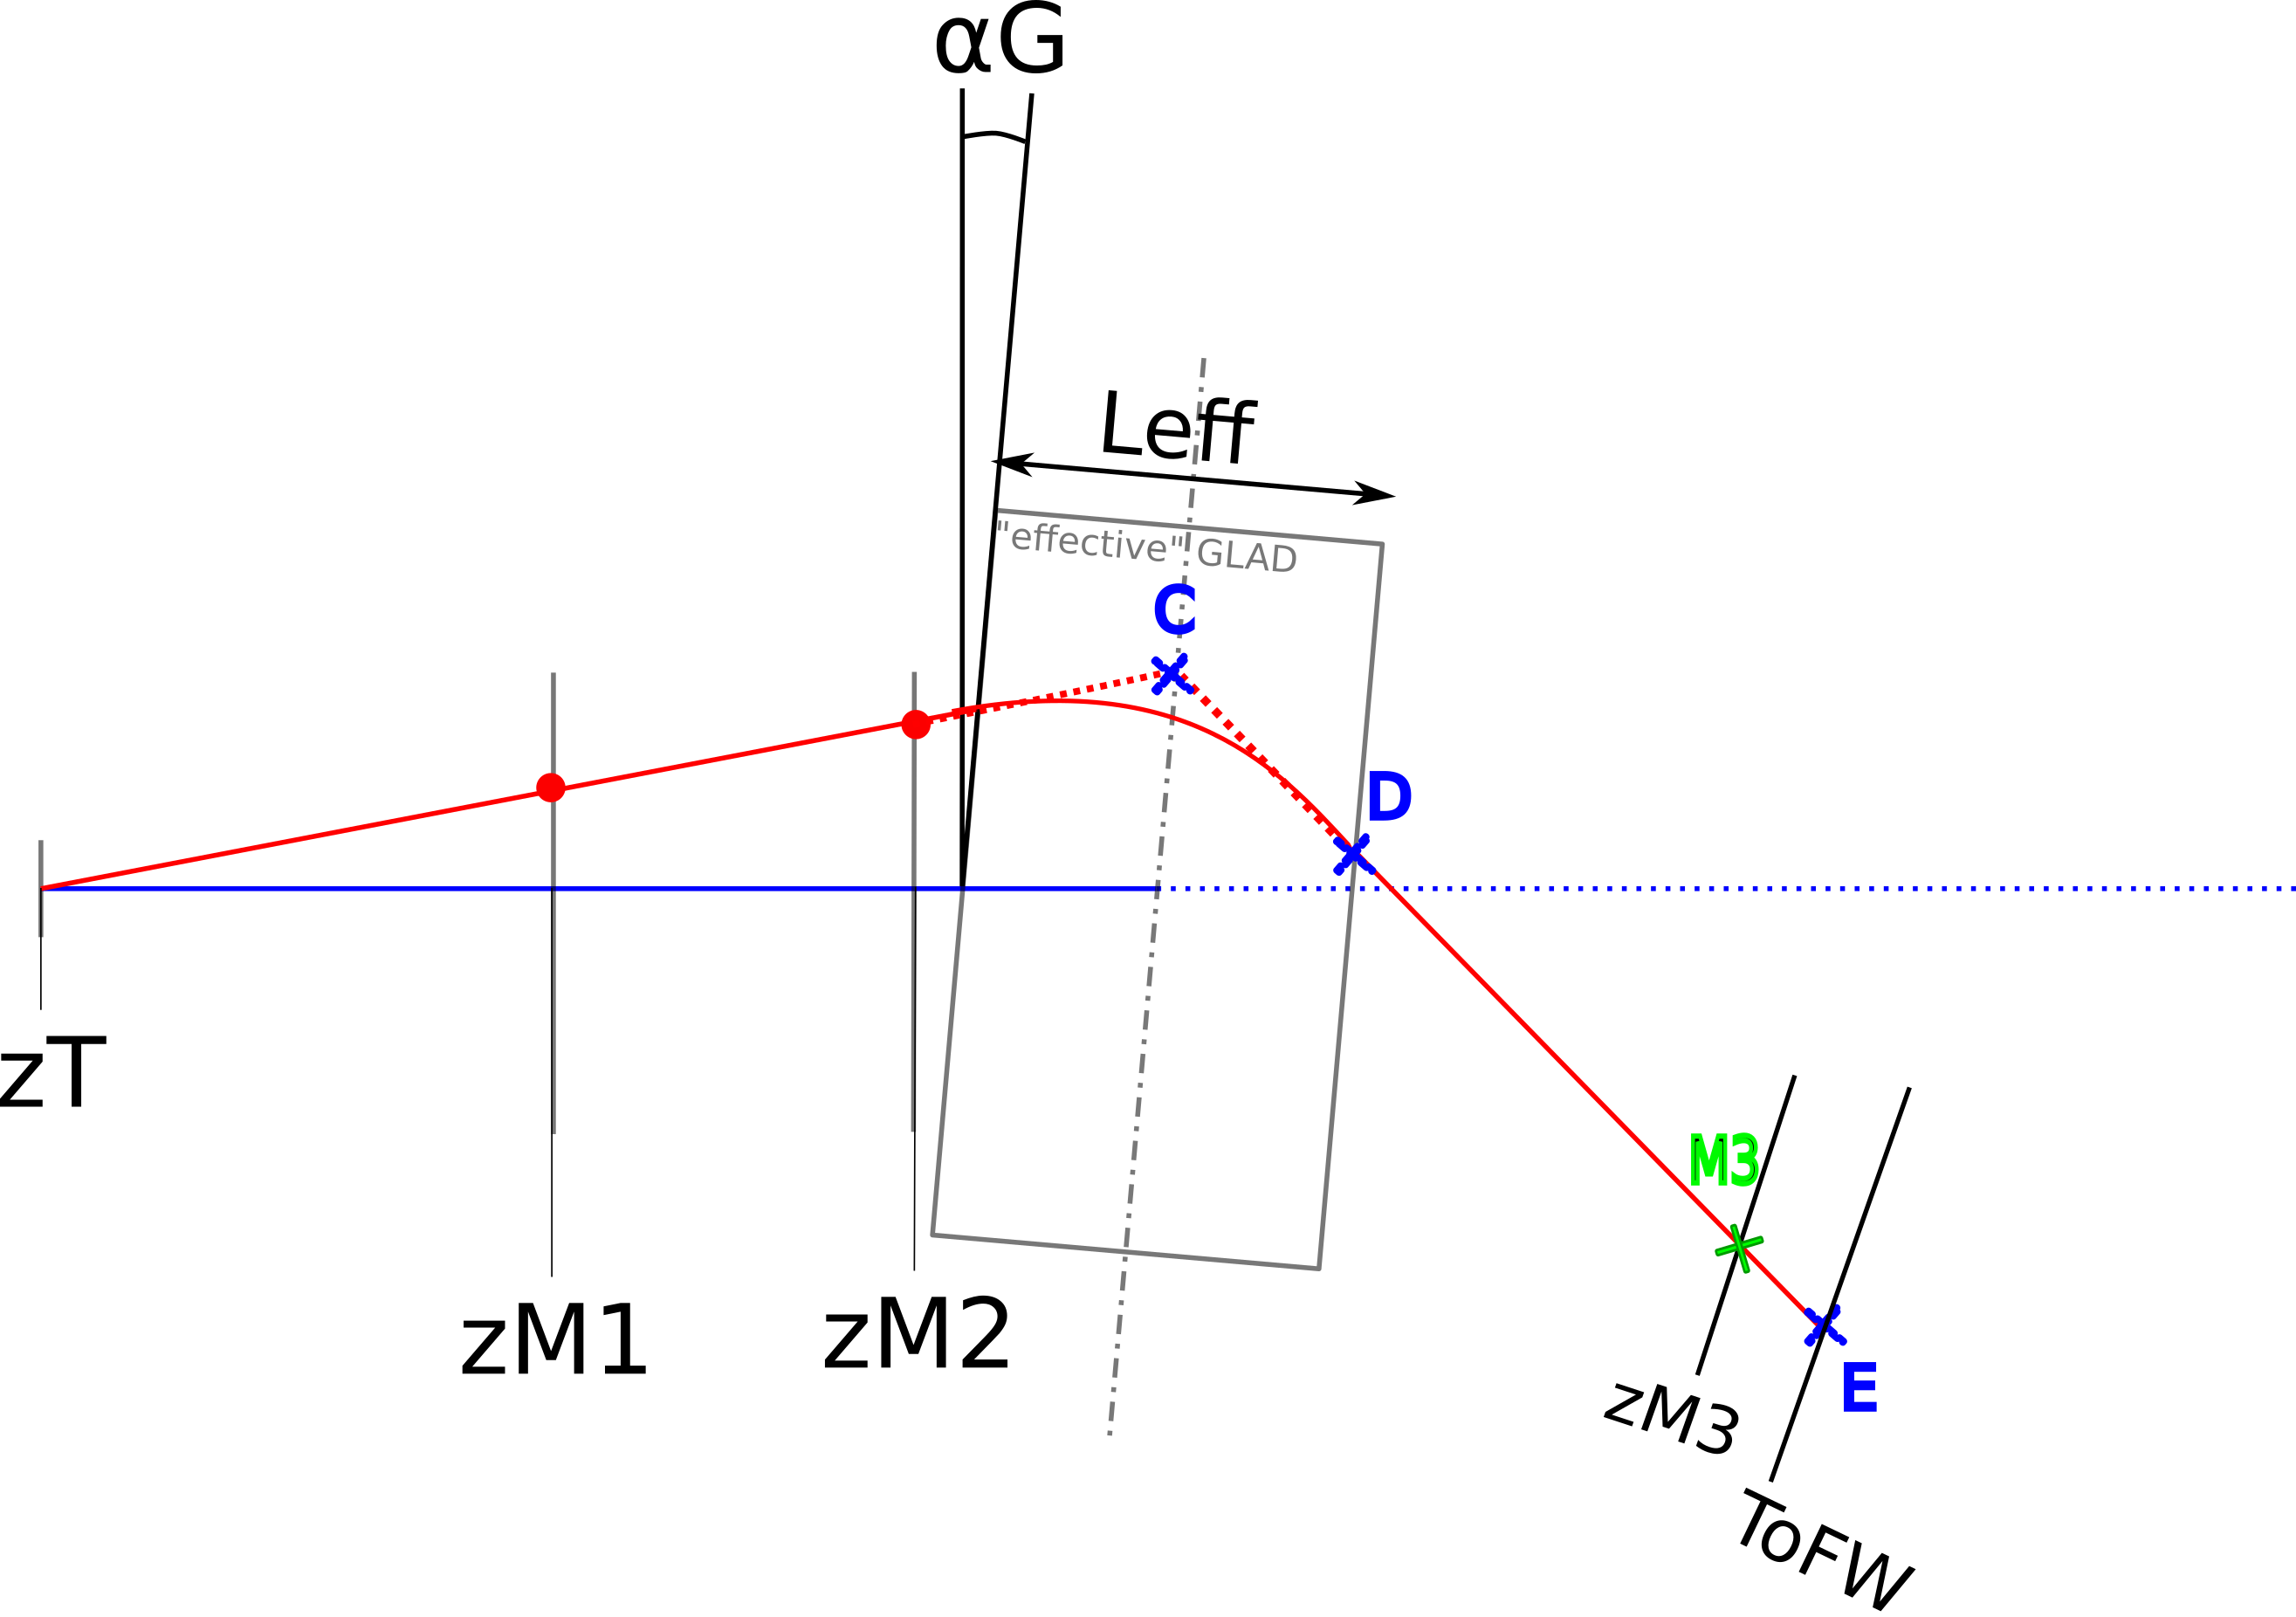
\includegraphics[width=1.0\textwidth]{tracking_downstreamGLAD.png}
\end{center}
\textbf{The straight line trajectory from D to E is definded by:}\\
\\
\textbf{$\Rightarrow$ the output angle from GLAD theta\textunderscore out}\\
\textbf{$\Rightarrow$ one absolute position after GLAD in the laboratory frame M3}\\
\\
With this information the straight line trajectory lenght after GLAD can be measured. It starts at the exit point of GLAD D and follows the straigh line (characterized by the angle theta\textunderscore out and the absolute position at MWPC3) until the intersection with the TofW ( middle position of the ToFWall zToFW$=6660.2 mm$, tilted angle$=18^{\circ}$).\\
\\
Finally the pathlength in the (x,z) plane from the target position to the ToFW is given by:\\
P = AB + $\rho\cdot\omega$ +DE\\
\\
where:\\
A = (x,z) position at the target point \\
B = (x,z) position at the GLAD entry point\\
D = (x,z) position at the GLAD exit point\\
E = (x,z) position where the constructed trajectory line hits the ToFW\\
\\
The assumption for the "Kickplane" method is that the kickpoint for each event lies on the predefinded Kickplane, the symmetry axis line of the GLAD magnet. 

\subsection{The "Fit-Track" method}
For the "Fit-Track" method the assumption that the kickpoint C lies on the symmetry axis line of the GLAD magnet is rejected. Instead following algorithm is applied: \footnote{This algorithm is motivated from \url{https://www.blogs.uni-mainz.de/fb08-kernphysik/files/2018/09/PHDThesis_OlgaBertini.pdf}, section $3.4$  }\\
\begin{enumerate}
\item Extend the line of flight of the ion before the GLAD.
\item Draw a line from the point MW3 to C (as constructed with the "Kickplane" method).
\item Now sweep the straight line after the kickpoint, leaving the position MW3 unchanged but sweeping the intersection point along the inline beam.
\item For each sweeping step plot theta\textunderscore out versus (d1-d2) where d1 is the distance betweeen B and the point of intersection and d2 the distance between D and the intersection point accordingly.
\item 50 sweeping steps are performed.
\item Fit the final theta\textunderscore out versus (d1-d2) plot with linear least square fit. 
\item Find the intersection of the abscissa. The corresponding theta\textunderscore out value is now the corrected one which should be used for the calculation of the radius.
\end{enumerate}
\begin{center}
	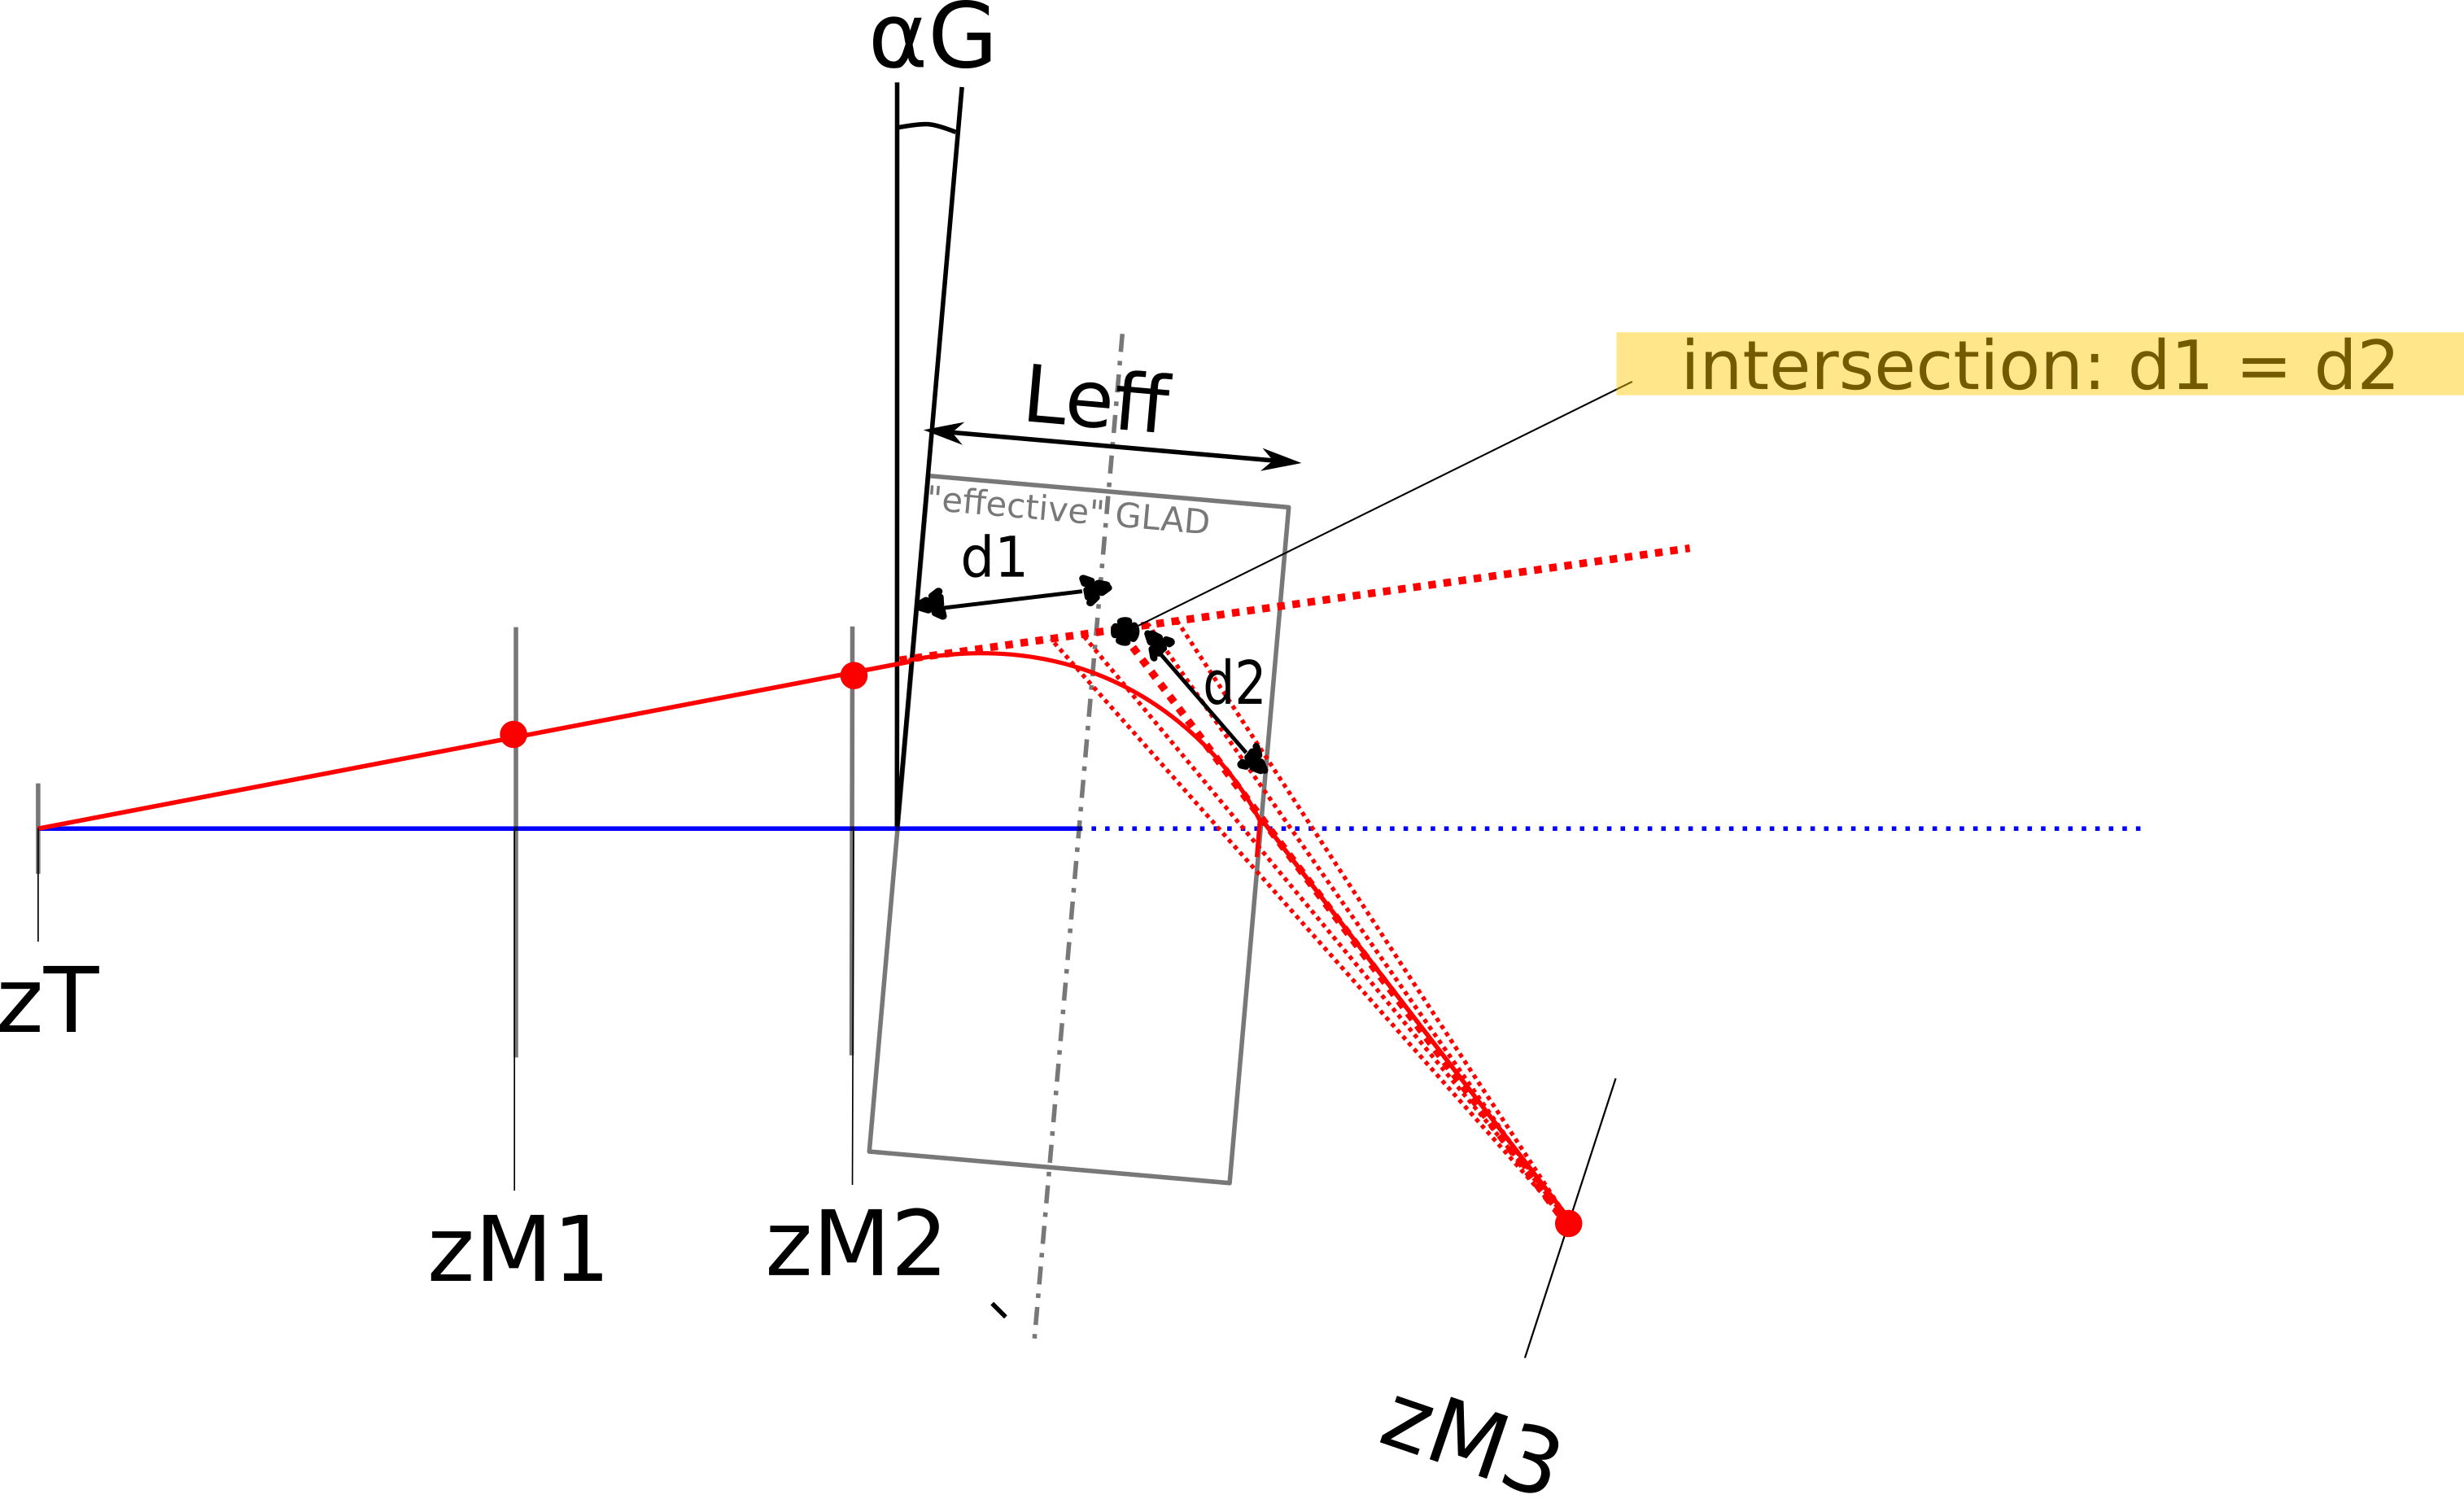
\includegraphics[width=1.0\textwidth]{tracking_alg_ALADIN_s.png}
\end{center}
\begin{center}
	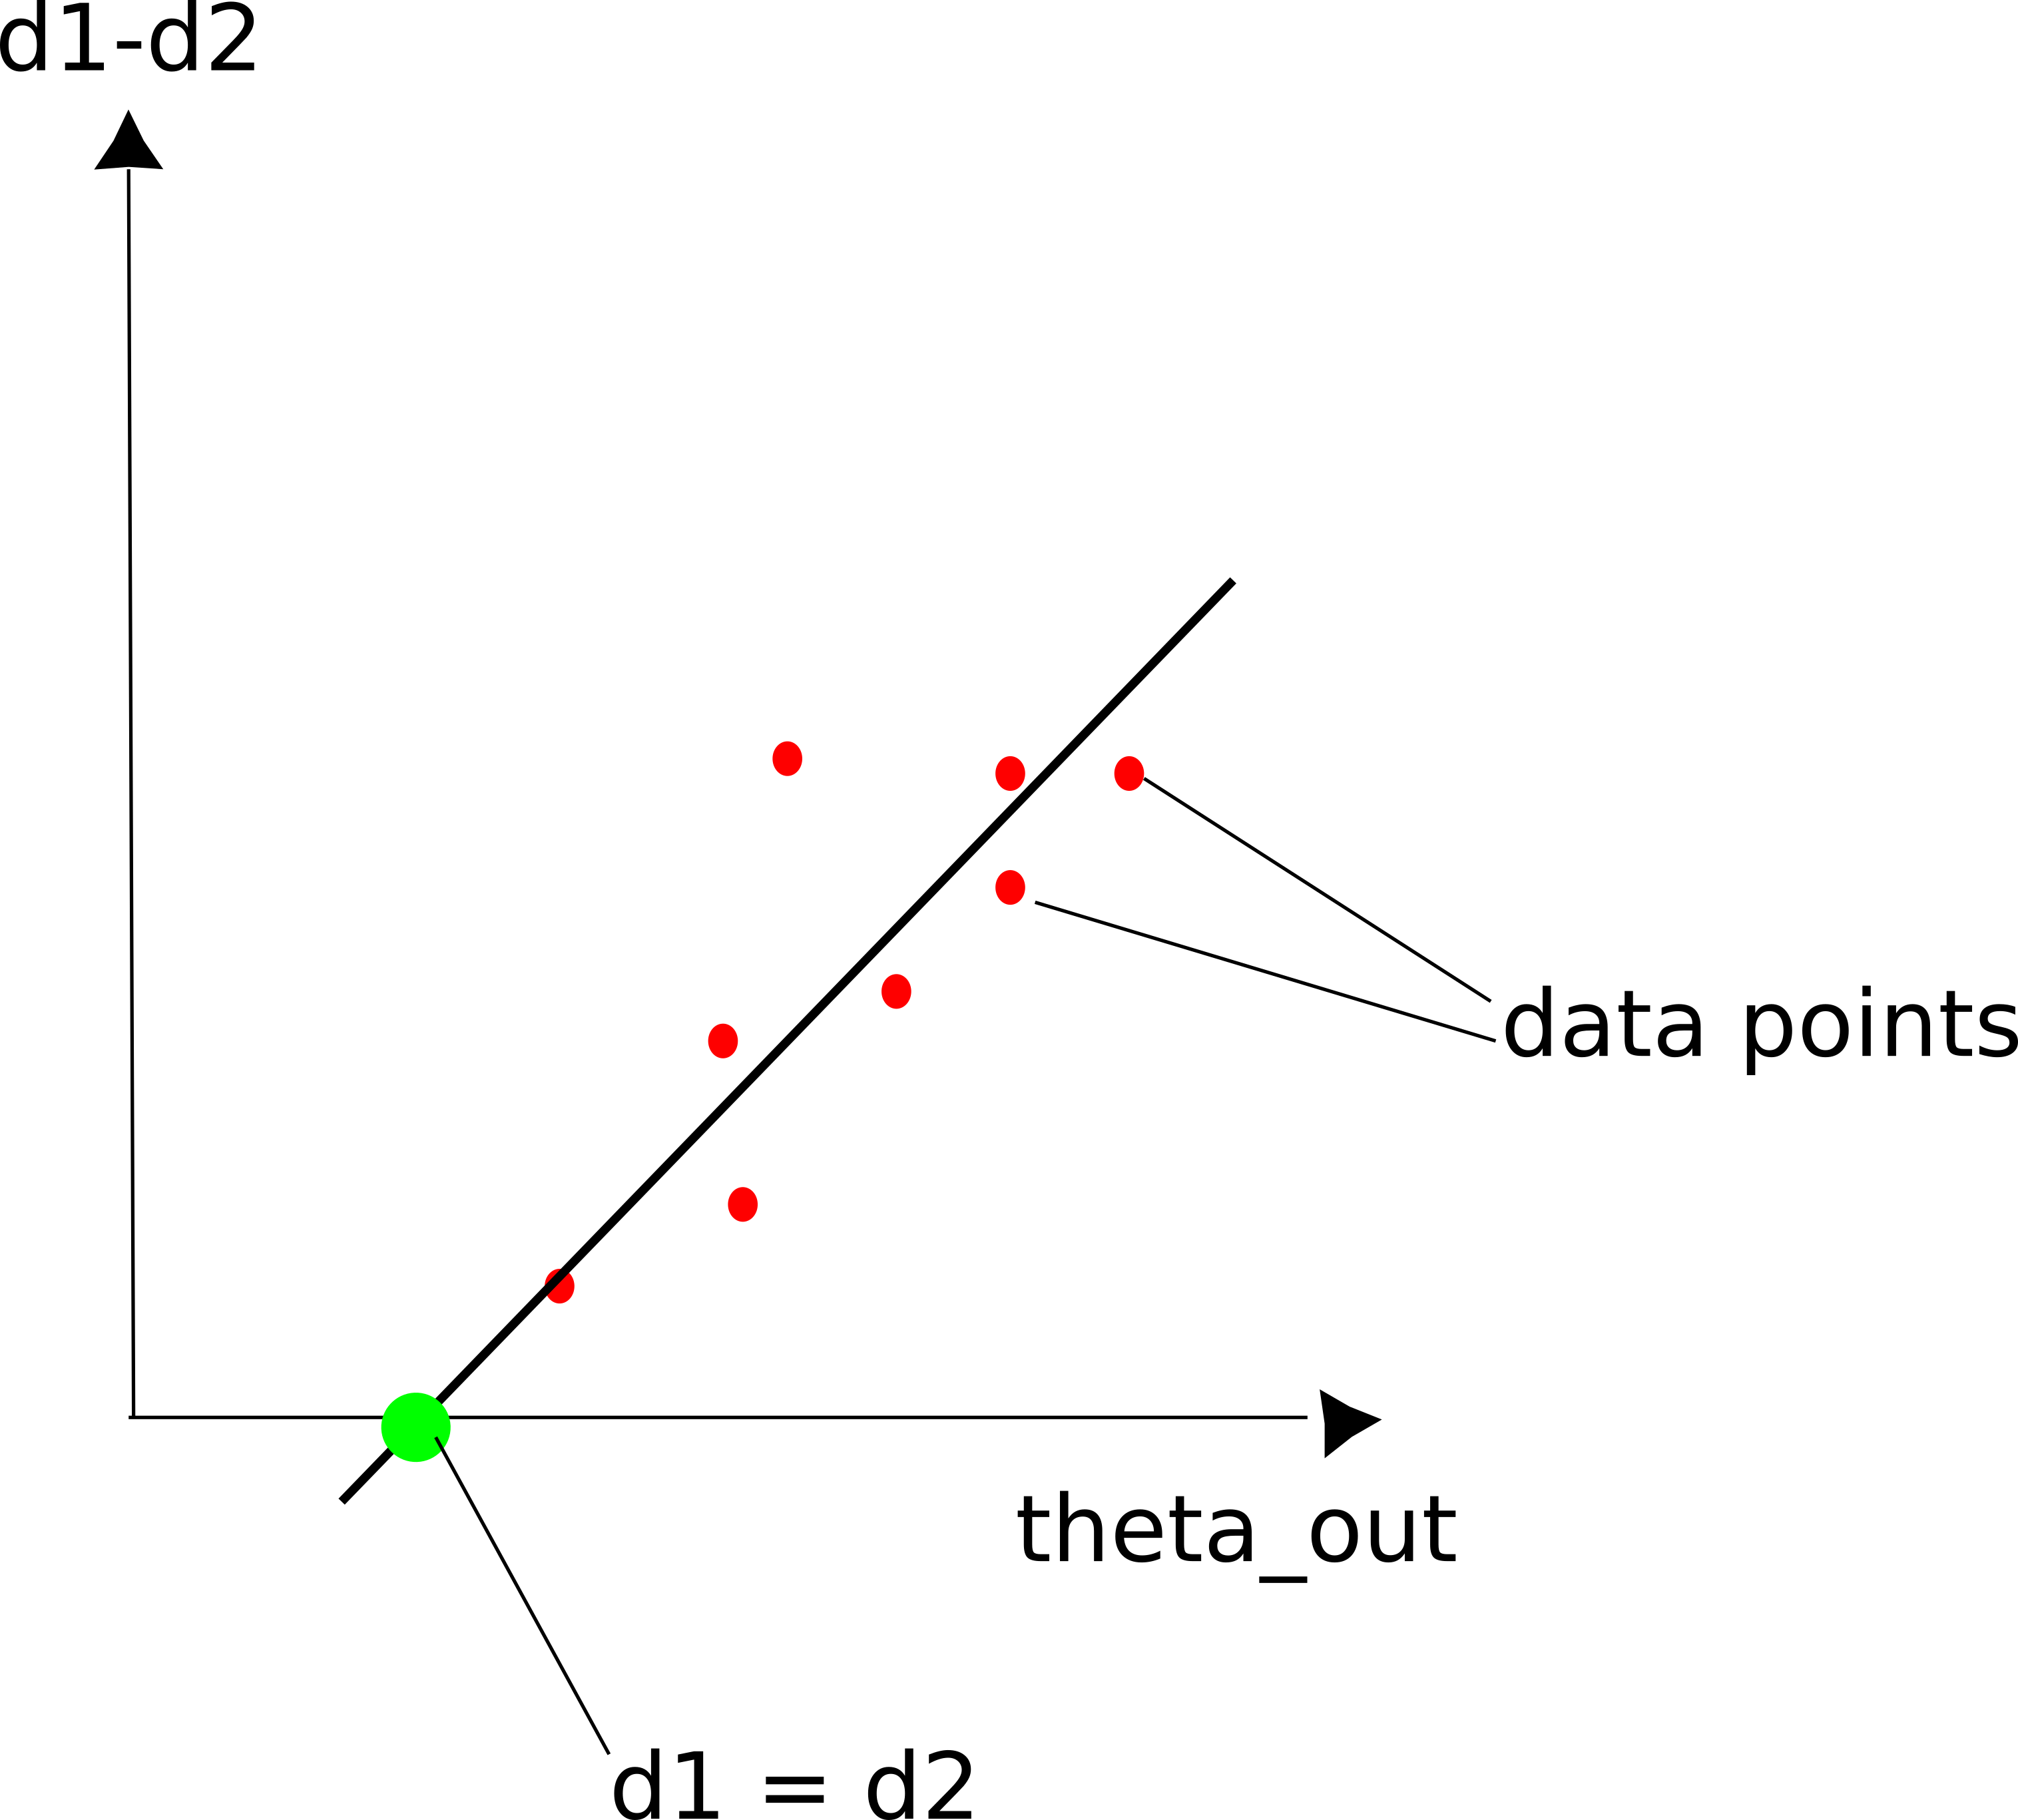
\includegraphics[width=0.5\textwidth]{theta_out_vs_d.png}
\end{center}


\subsection{The "Theta\textunderscore in correction" method}

Here the "Kickplane" method is used and subsequently the theta\textunderscore out is corrected by  theta\textunderscore in. That means:\\
\\
theta\textunderscore out\textunderscore corr = theta\textunderscore out - theta\textunderscore in.\\
\\
Consequentely the theta\textunderscore in dependence of $\rho$ vanishes(neglecting the $\cos(\delta)$ term):\\
\\

$\rho$ = $\frac{\textrm{L\textunderscore eff}}{2\cdot\sin\left(\frac{theta\textunderscore in}{2} +\frac{theta\textunderscore out\textunderscore corr}{2}\right)} = \frac{\textrm{L\textunderscore eff}}{2\cdot\sin\left(\frac{theta\textunderscore out}{2}\right)}$
\begin{center}
	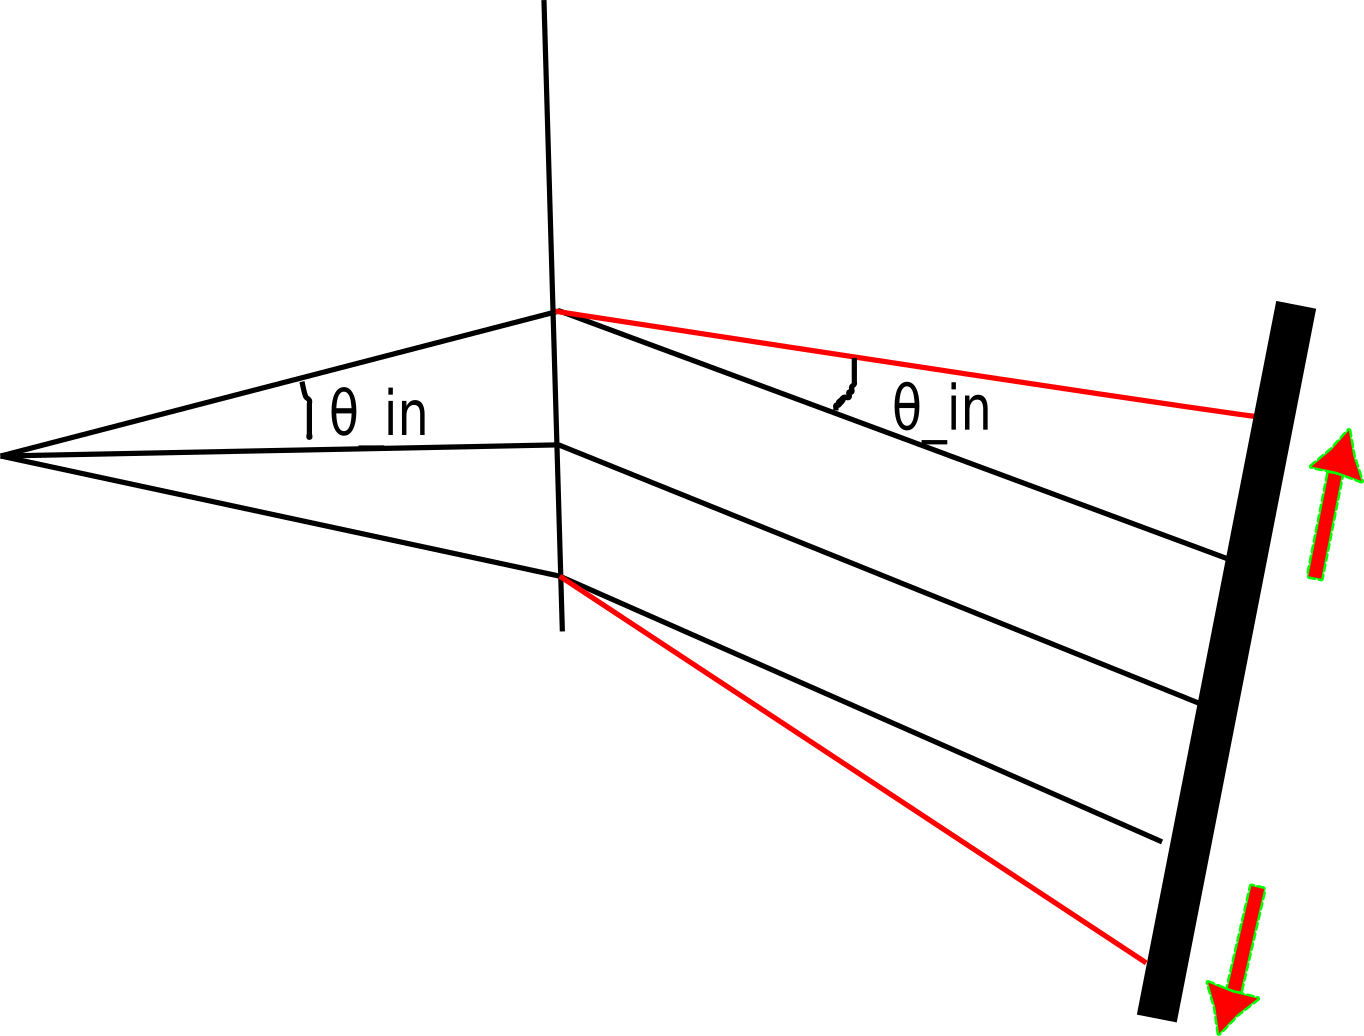
\includegraphics[width=0.7\textwidth]{theta_out_corr_alg.png}
\end{center}

\subsection{Final method: "Advanced Fit-Track" method}
The same track finding algorithm as for the "Fit-Track" method is used with the only difference that the value for $theta\textunderscore in$ is calculated from the fit of $theta\textunderscore out$ vs. xMW3:\\
%insert plot here with fit theta_out vs xMW3
\\
The parameters of the linear fit are used for the calculation of $theta\textunderscore in$ :\\

$theta\textunderscore in = \alpha - a \cdot x\textunderscore MW3 - b$ \\
\\
With \textbf{a} being the slope and \textbf{b} the offset of the fit. This method prevents from adding up the errors from theta\textunderscore in measurement.\\
$\alpha$ corresponds to the mean value of the theta \textunderscore out from the fit of $theta\textunderscore out$ vs. xMW3.

\section{Plots}
In this section all the plots for the various track finding algorithms are presented. For the calculation of the theta\textunderscore in angle MWPC1 and MWPC2 are used. Alternatively MWPC0 and MWPC2 could be used, to get a longer lever arm (work in progress ...).\\

\subsection{MWPC1 vs MWPC2 - x position}
\begin{figure}[!htbp]
\begin{subfigure}{.5\textwidth}
  \centering
  % include first image
  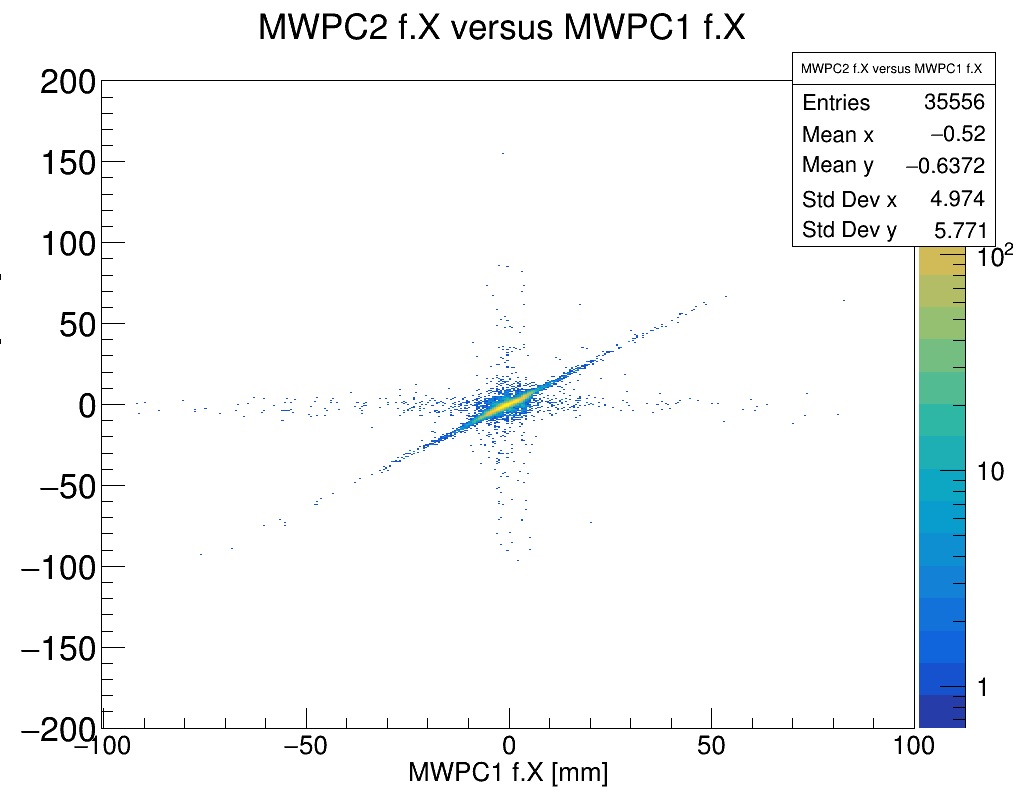
\includegraphics[width=.9\linewidth]{plot_imgs/mw2_mw1_get_centr.png}  
  \caption{"Kickplane-Method"}
  \label{fig:sub-first}
\end{subfigure}
\begin{subfigure}{.5\textwidth}
  \centering
  % include second image
  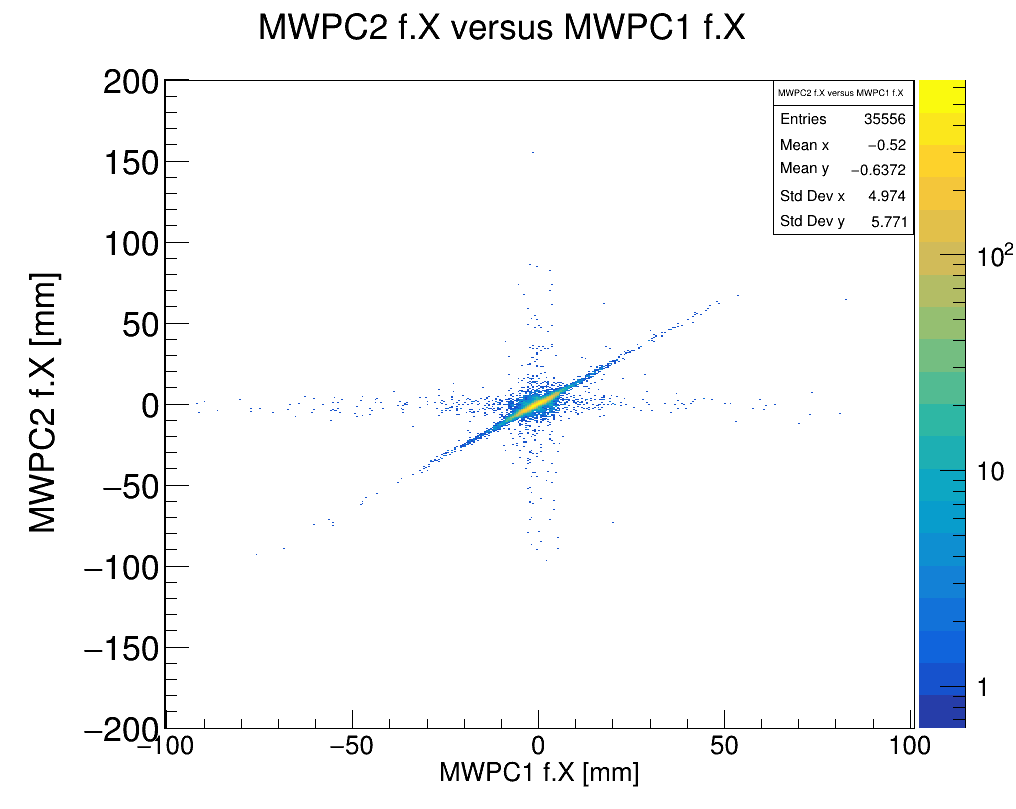
\includegraphics[width=.9\linewidth]{plot_imgs/mw2_mw1_corr.png} 
  \caption{"Theta \textunderscore in correction-Method"}
  \label{fig:sub-second}
\end{subfigure}
\begin{subfigure}{.5\textwidth}
  \centering
  % include second image
  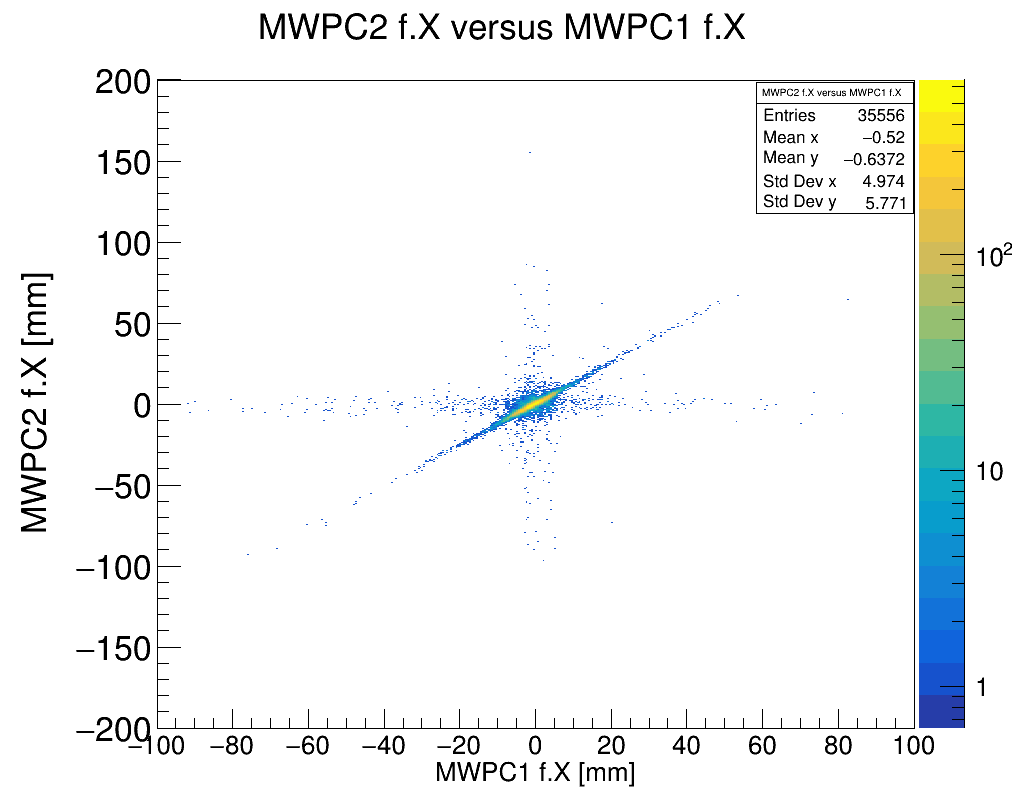
\includegraphics[width=.9\linewidth]{plot_imgs/mw2_mw1_fit.png} 
  \caption{"Fit-Track-Method"}
  \label{fig:sub-second}
\end{subfigure}
\begin{subfigure}{.5\textwidth}
  \centering
  % include second image
  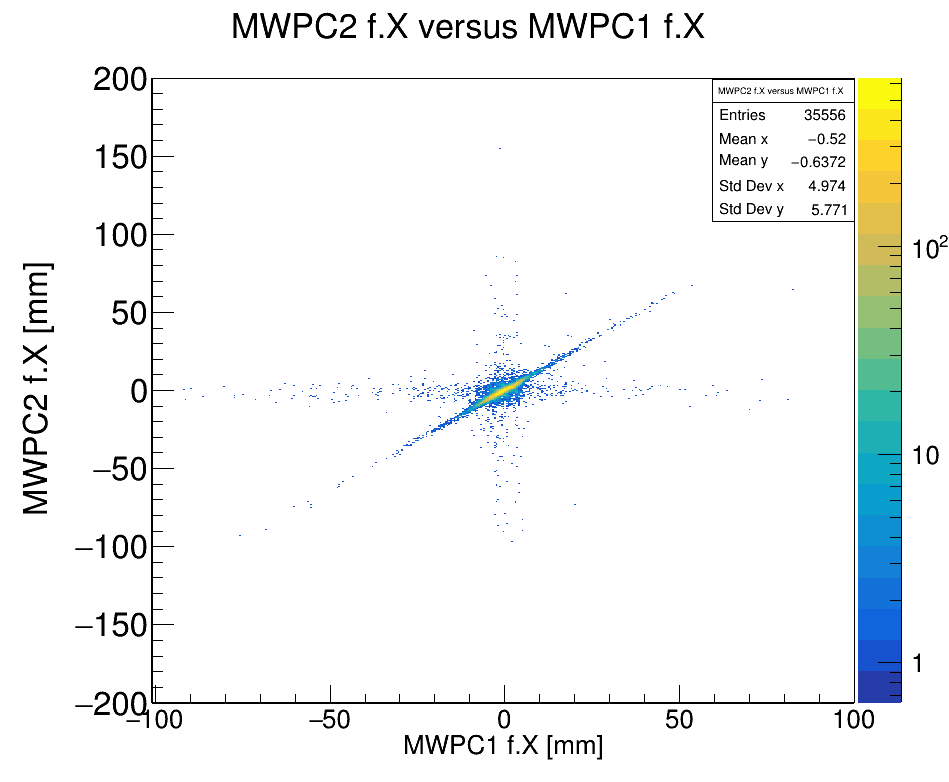
\includegraphics[width=.9\linewidth]{plot_imgs/mw2_mw1_alpha.png} 
  \caption{"Advanced Fit-Track-Method"}
  \label{fig:sub-second}
\end{subfigure}
\caption{MWPC1 vs MPWPC2 - x position for sweep runs 39-61.}
\label{fig:fig}
\end{figure}
\FloatBarrier
\clearpage
\subsection{MW0 vs MW2- x position }
\begin{figure}[!htbp]
\begin{subfigure}{.5\textwidth}
  \centering
  % include first image
  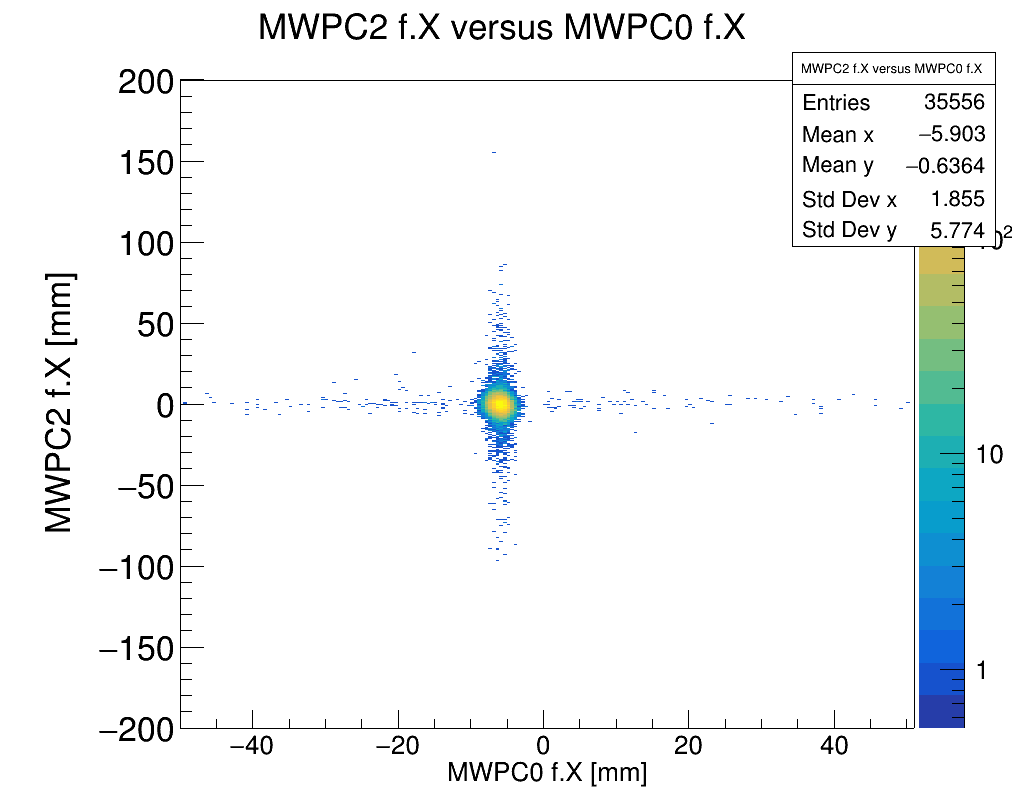
\includegraphics[width=.9\linewidth]{plot_imgs/mw2_mw0_get_centr.png}  
  \caption{"Kickplane-Method"}
  \label{fig:sub-first}
\end{subfigure}
\begin{subfigure}{.5\textwidth}
  \centering
  % include second image
  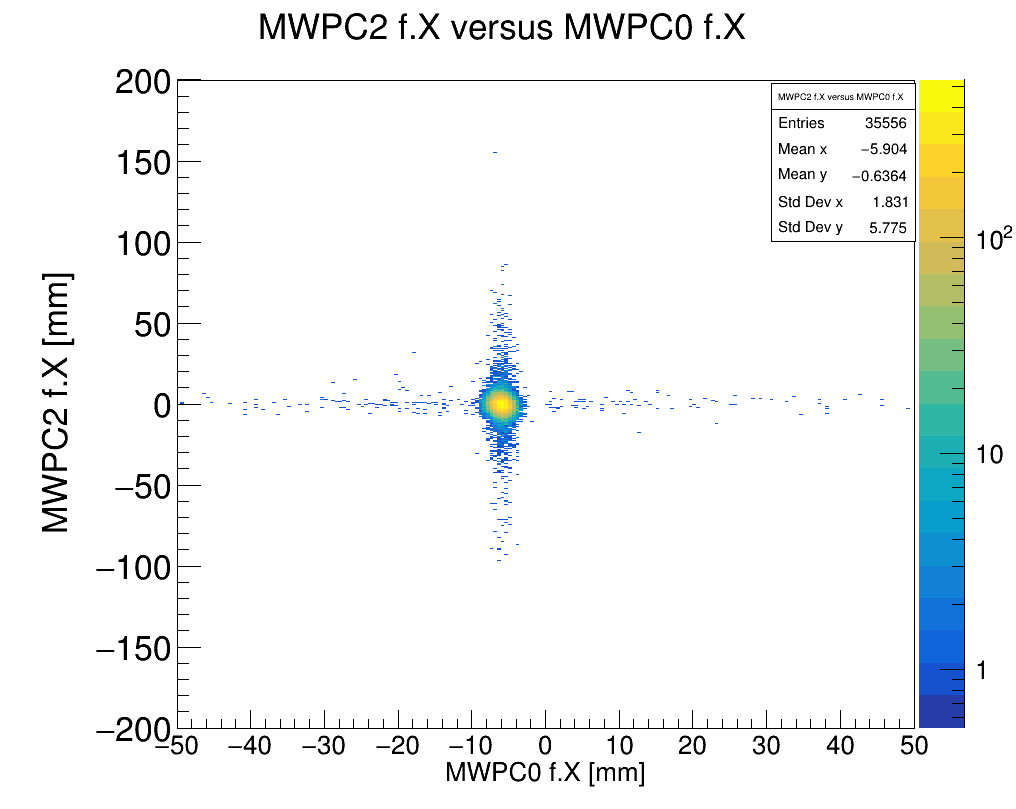
\includegraphics[width=.9\linewidth]{plot_imgs/mw2_mw0_corr.png} 
  \caption{"Theta \textunderscore in correction-Method"}
  \label{fig:sub-second}
\end{subfigure}
\begin{subfigure}{.5\textwidth}
  \centering
  % include second image
  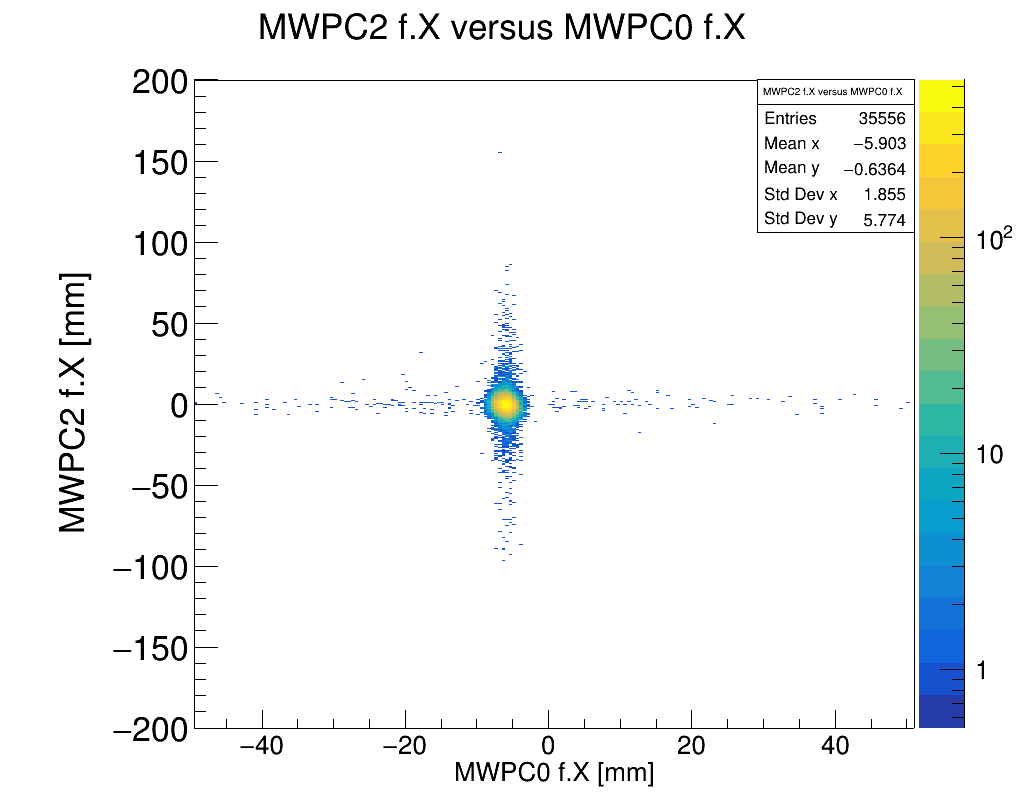
\includegraphics[width=.9\linewidth]{plot_imgs/mw2_mw0_fit.png} 
  \caption{"Fit-Track-Method"}
  \label{fig:sub-second}
\end{subfigure}
\begin{subfigure}{.5\textwidth}
  \centering
  % include second image
  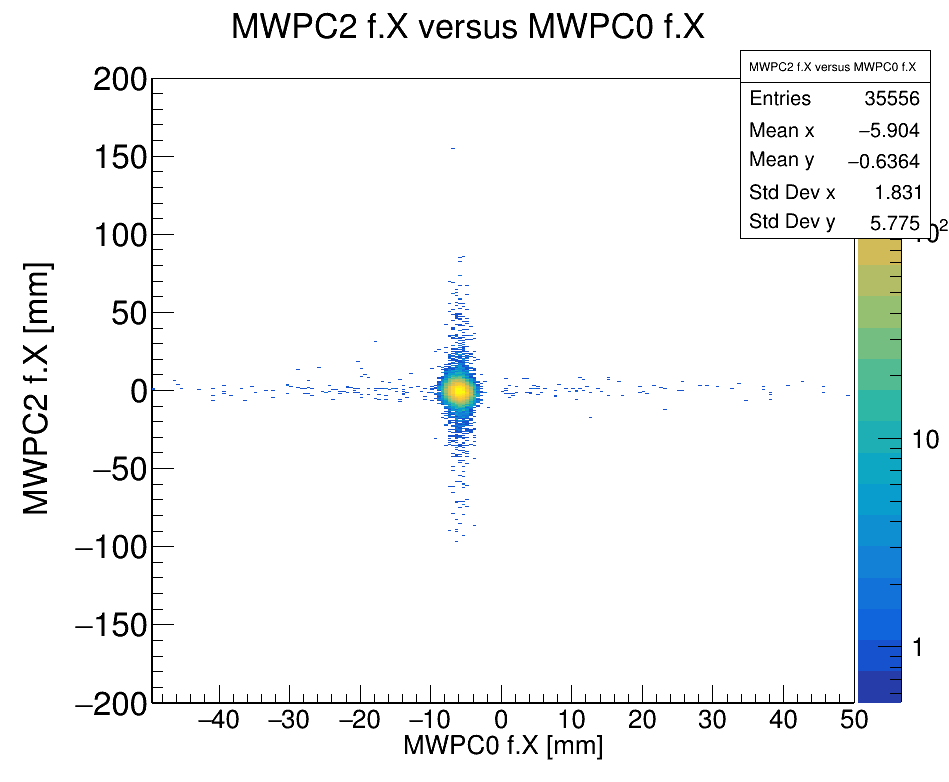
\includegraphics[width=.9\linewidth]{plot_imgs/mw2_mw0_alpha.png} 
  \caption{"Advanced Fit-Track-Method"}
  \label{fig:sub-second}
\end{subfigure}
\caption{MWPC2 vs MWPC0 - x position for sweep runs 39-61.}
\label{fig:fig}
\end{figure}
\FloatBarrier
\clearpage
\subsection{MW1 vs MW3 - x position}
\begin{figure}[!htbp]
\begin{subfigure}{.5\textwidth}
  \centering
  % include first image
  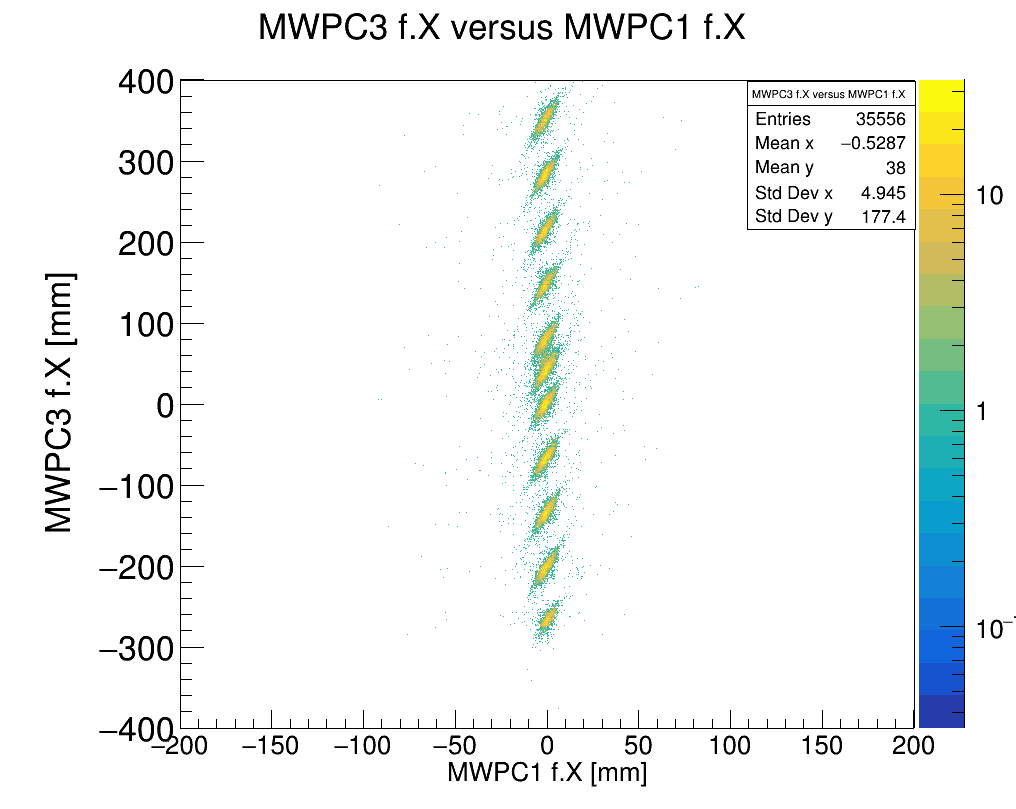
\includegraphics[width=.9\linewidth]{plot_imgs/mw3_mw1_get_centr.png}  
  \caption{"Kickplane-Method"}
  \label{fig:sub-first}
\end{subfigure}
\begin{subfigure}{.5\textwidth}
  \centering
  % include second image
  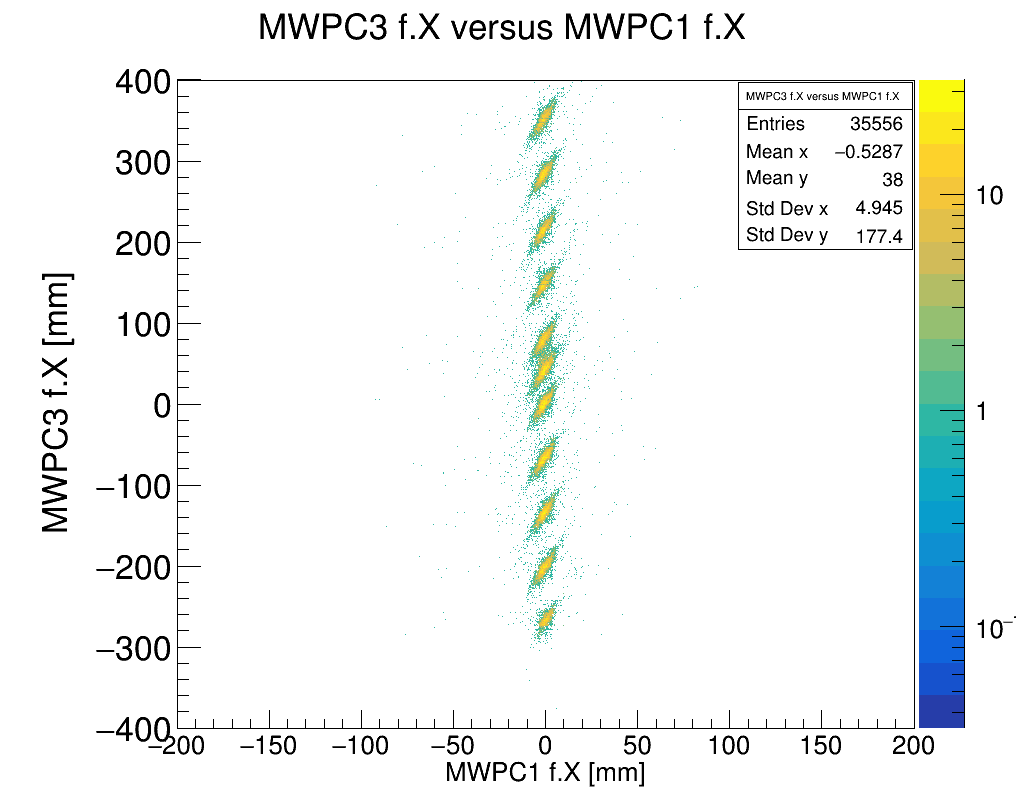
\includegraphics[width=.9\linewidth]{plot_imgs/mw3_mw1_corr.png} 
  \caption{"Theta \textunderscore in correction-Method"}
  \label{fig:sub-second}
\end{subfigure}
\begin{subfigure}{.5\textwidth}
  \centering
  % include second image
  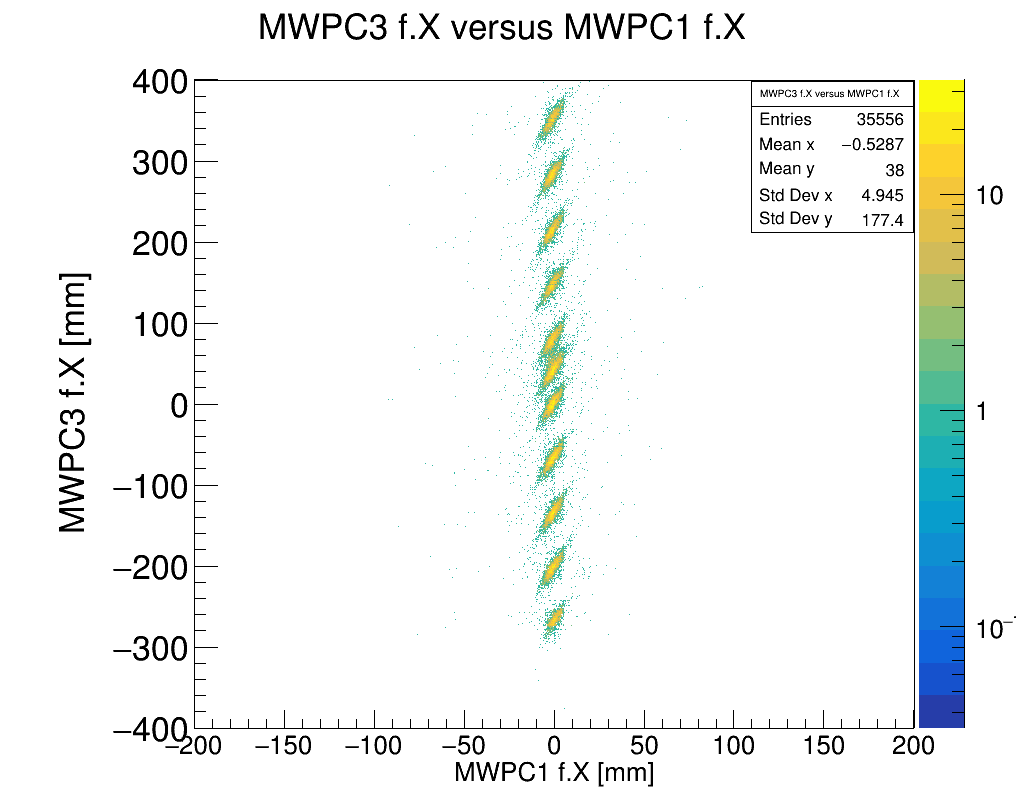
\includegraphics[width=.9\linewidth]{plot_imgs/mw3_mw1_fit.png} 
  \caption{"Fit-Track-Method"}
  \label{fig:sub-second}
\end{subfigure}
\begin{subfigure}{.5\textwidth}
  \centering
  % include second image
  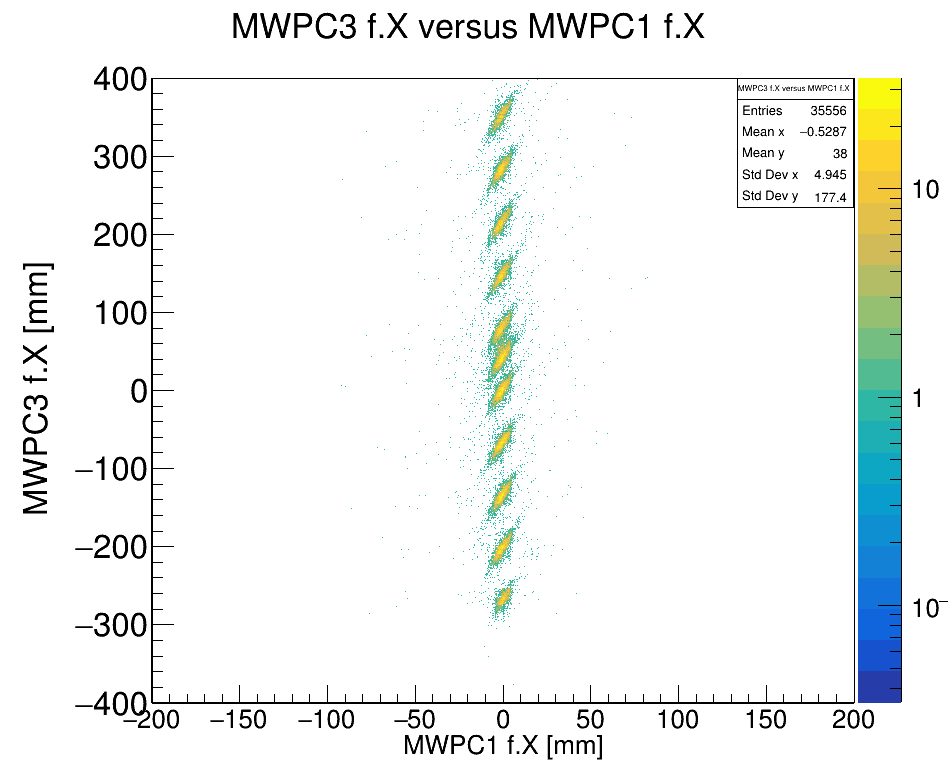
\includegraphics[width=.9\linewidth]{plot_imgs/mw3_mw1_alpha.png} 
  \caption{"Advanced Fit-Track-Method"}
  \label{fig:sub-second}
\end{subfigure}
\caption{MWPC3 vs MWPC1 - x position for sweep runs 39-61.}
\label{fig:fig}
\end{figure}
\FloatBarrier
\clearpage
\subsection{theta\textunderscore out vs MW3- x position }
\begin{figure}[!htbp]
\begin{subfigure}{.5\textwidth}
  \centering
  % include first image
  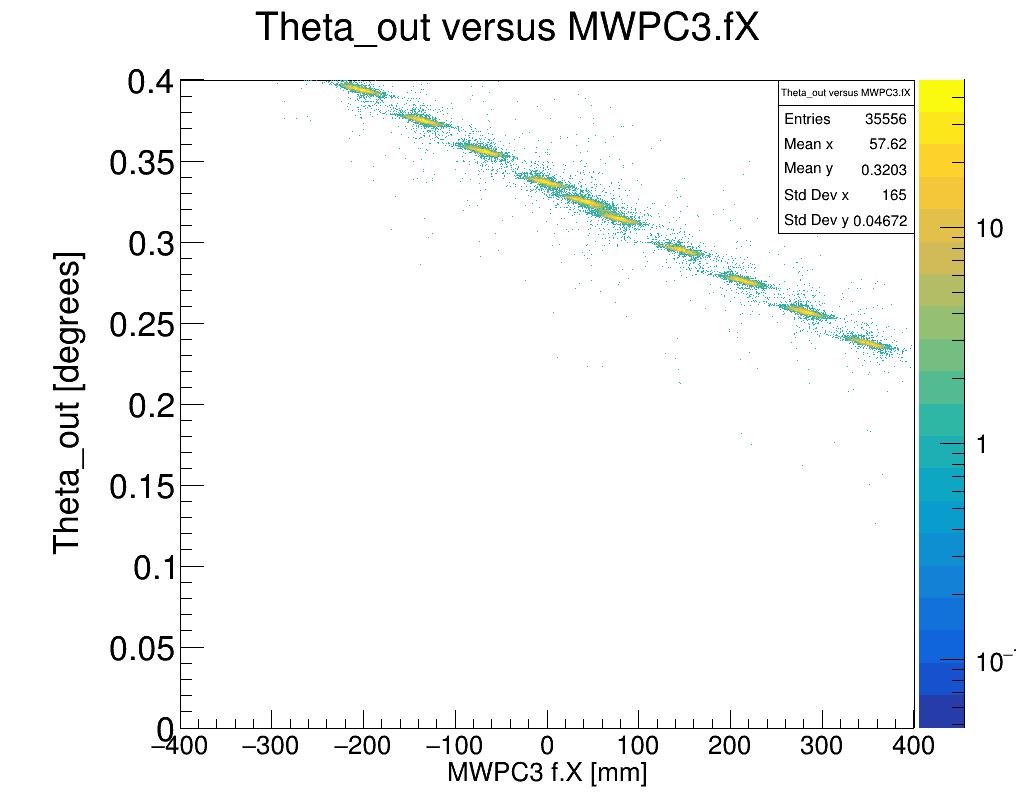
\includegraphics[width=.9\linewidth]{plot_imgs/theta_out_mw3_get_centr.png}  
  \caption{"Kickplane-Method"}
  \label{fig:sub-first}
\end{subfigure}
\begin{subfigure}{.5\textwidth}
  \centering
  % include second image
  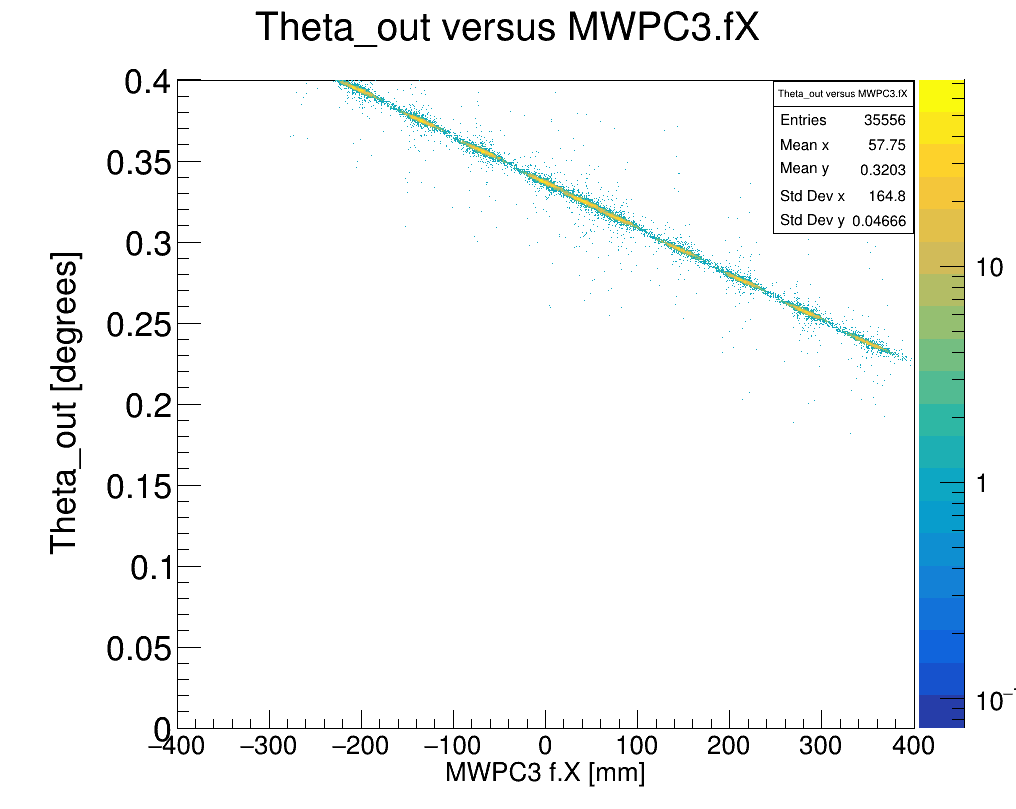
\includegraphics[width=.9\linewidth]{plot_imgs/theta_out_mw3_corr.png} 
  \caption{"Theta \textunderscore in correction-Method"}
  \label{fig:sub-second}
\end{subfigure}
\begin{subfigure}{.5\textwidth}
  \centering
  % include second image
  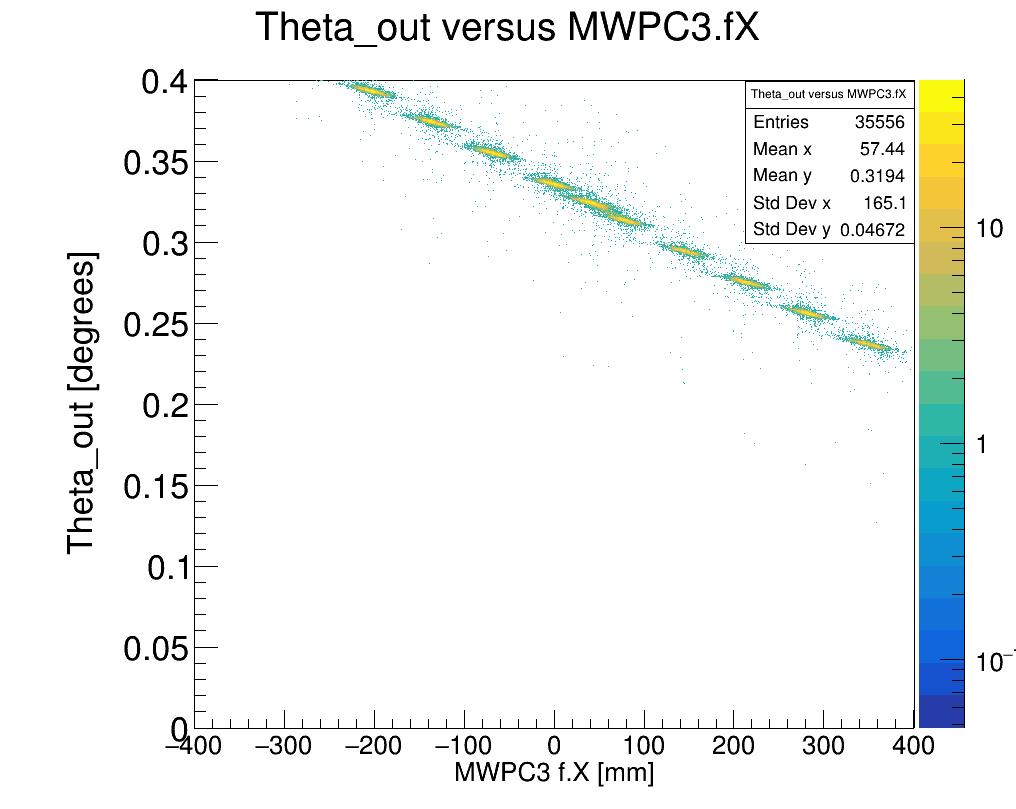
\includegraphics[width=.9\linewidth]{plot_imgs/theta_out_mw3_fit.png} 
  \caption{"Fit-Track-Method"}
  \label{fig:sub-second}
\end{subfigure}
\begin{subfigure}{.5\textwidth}
  \centering
  % include second image
  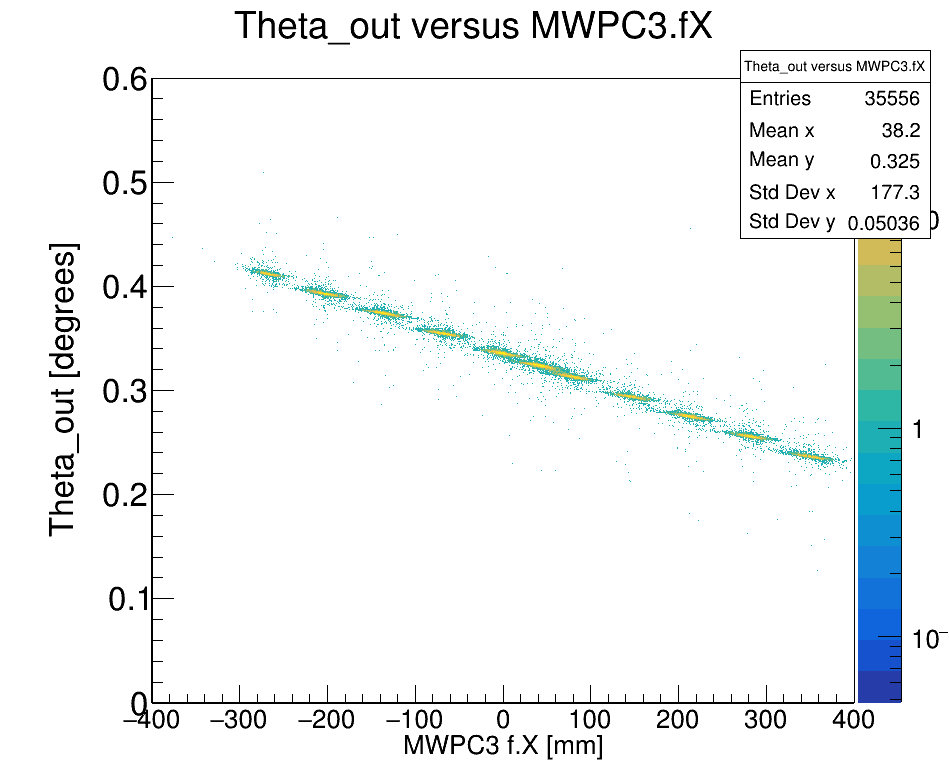
\includegraphics[width=.9\linewidth]{plot_imgs/theta_out_mw3_alpha.png} 
  \caption{"Advanced Fit-Track-Method"}
  \label{fig:sub-second}
\end{subfigure}
\caption{Theta\textunderscore out vs MWPC3 x position for sweep runs 39-61.}
\label{fig:fig}
\end{figure}
\FloatBarrier
\clearpage
\subsection{theta\textunderscore in vs MW3 - x position}
\begin{figure}[!htbp]
\begin{subfigure}{.5\textwidth}
  \centering
  % include first image
  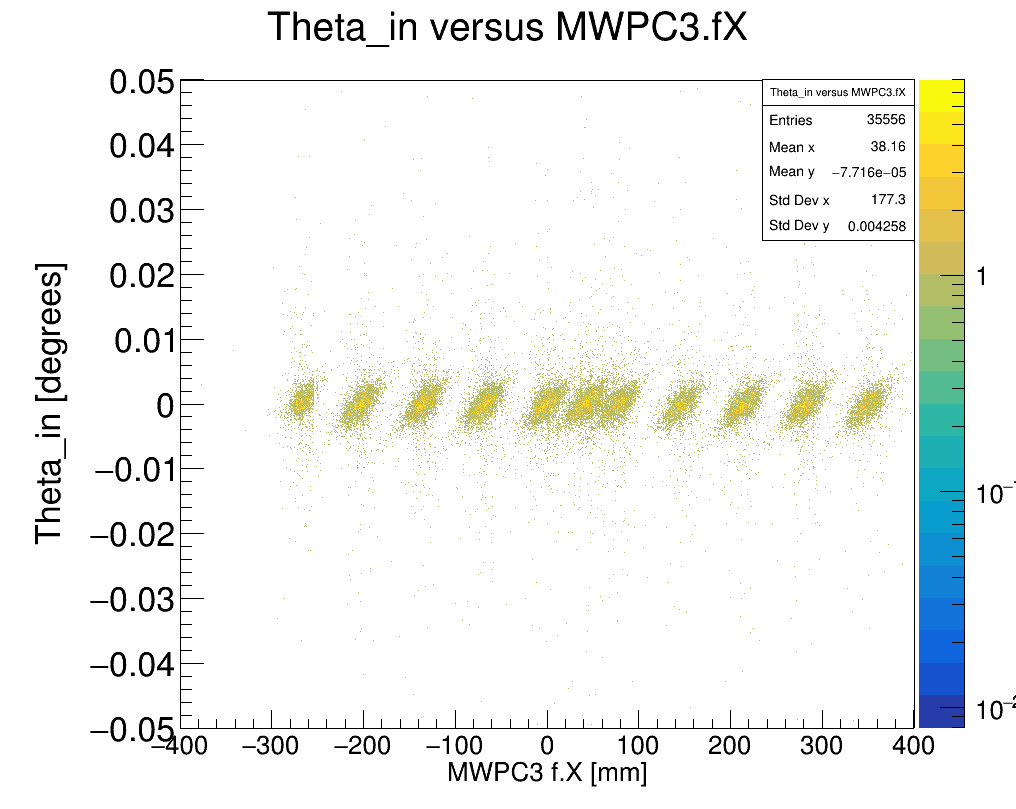
\includegraphics[width=.9\linewidth]{plot_imgs/theta_in_mw3_get_centr.png}  
  \caption{"Kickplane-Method"}
  \label{fig:sub-first}
\end{subfigure}
\begin{subfigure}{.5\textwidth}
  \centering
  % include second image
  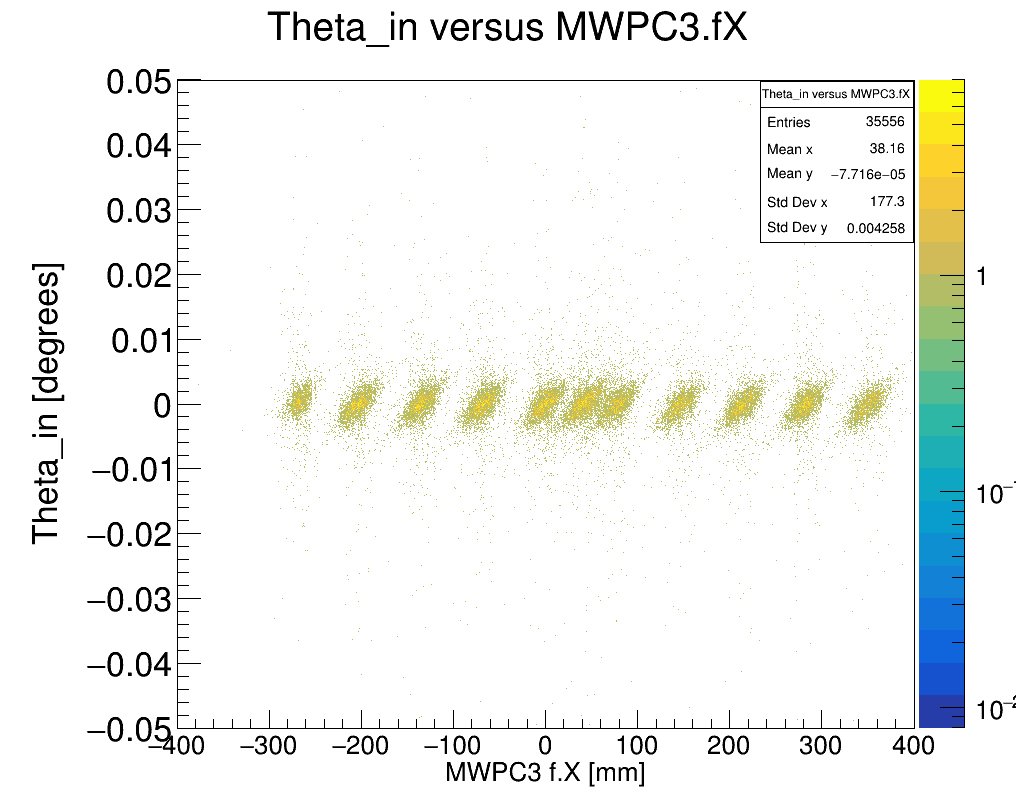
\includegraphics[width=.9\linewidth]{plot_imgs/theta_in_mw3_corr.png} 
  \caption{"Theta \textunderscore in correction-Method"}
  \label{fig:sub-second}
\end{subfigure}
\begin{subfigure}{.5\textwidth}
  \centering
  % include second image
  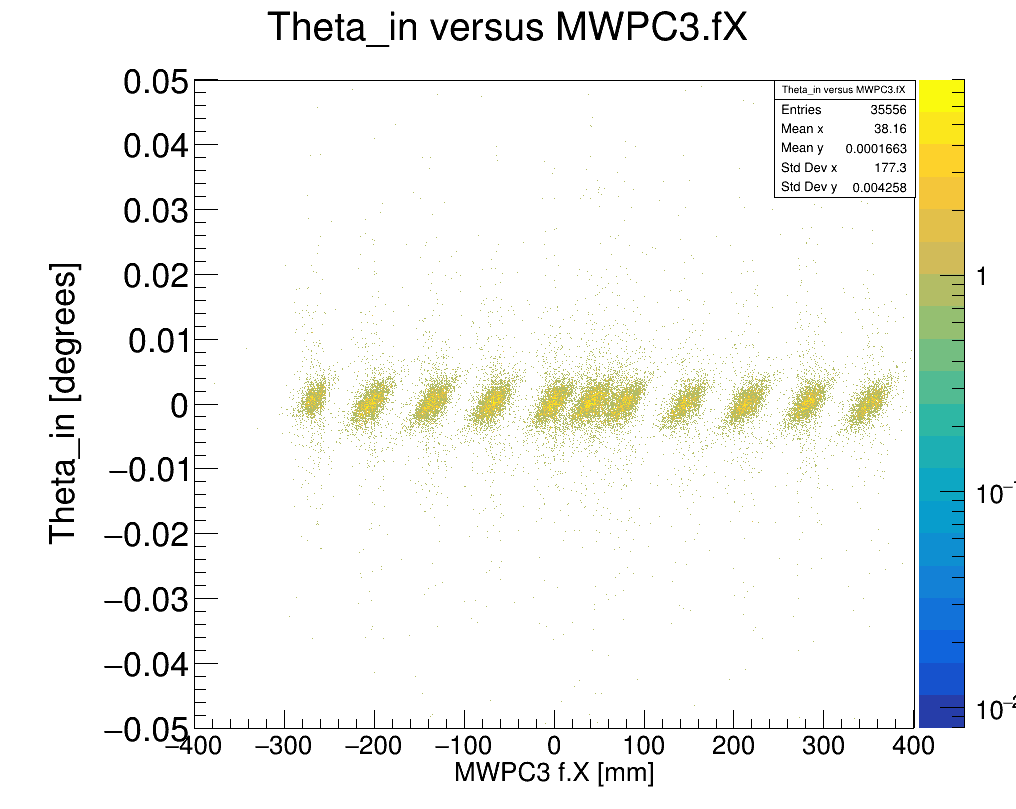
\includegraphics[width=.9\linewidth]{plot_imgs/theta_in_mw3_fit.png} 
  \caption{"Fit-Track-Method"}
  \label{fig:sub-second}
\end{subfigure}
\begin{subfigure}{.5\textwidth}
  \centering
  % include second image
  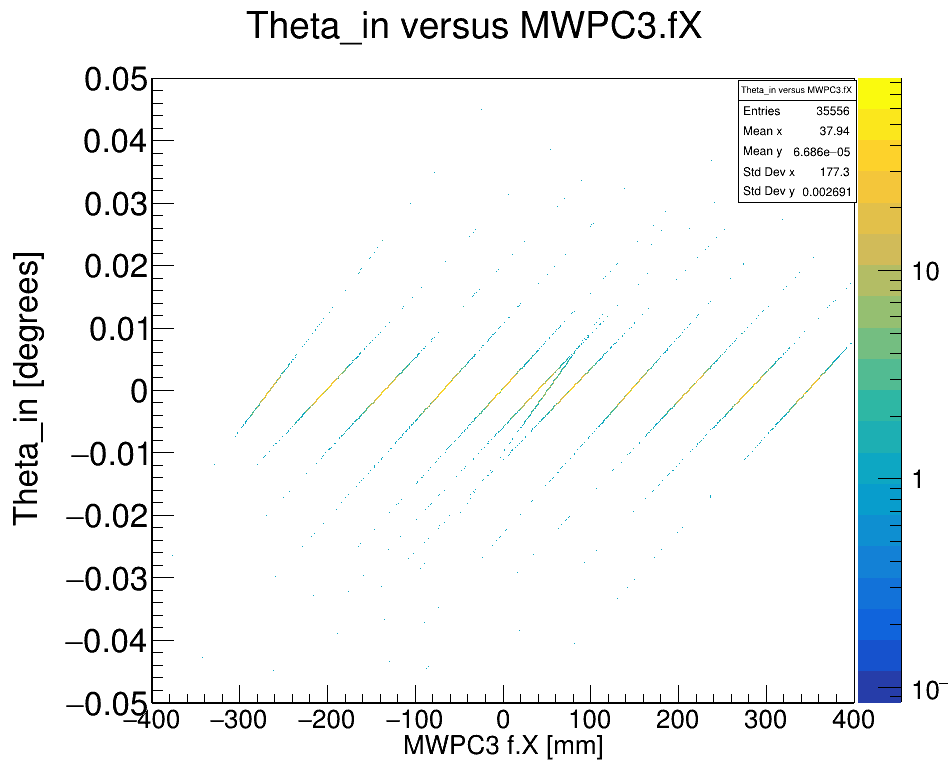
\includegraphics[width=.9\linewidth]{plot_imgs/theta_in_mw3_alpha.png} 
  \caption{"Advanced Fit-Track-Method"}
  \label{fig:sub-second}
\end{subfigure}
\caption{Theta \textunderscore in vs MWPC3 x position for sweep runs 39-61.}
\label{fig:fig}
\end{figure}
\FloatBarrier
\clearpage
\subsection{theta\textunderscore in+theta\textunderscore out vs MW3- x position }
\begin{figure}[!htbp]
\begin{subfigure}{.5\textwidth}
  \centering
  % include first image
  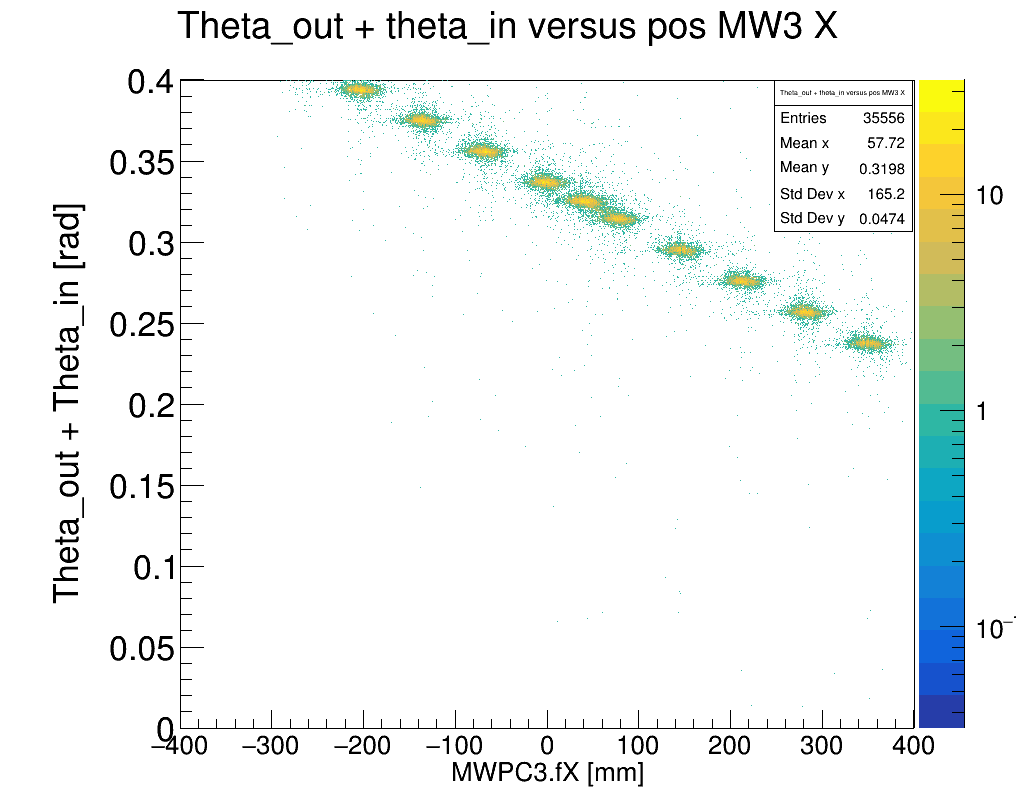
\includegraphics[width=.9\linewidth]{plot_imgs/theta_out_theta_in_mw3_get_centr.png}  
  \caption{"Kickplane-Method"}
  \label{fig:sub-first}
\end{subfigure}
\begin{subfigure}{.5\textwidth}
  \centering
  % include second image
  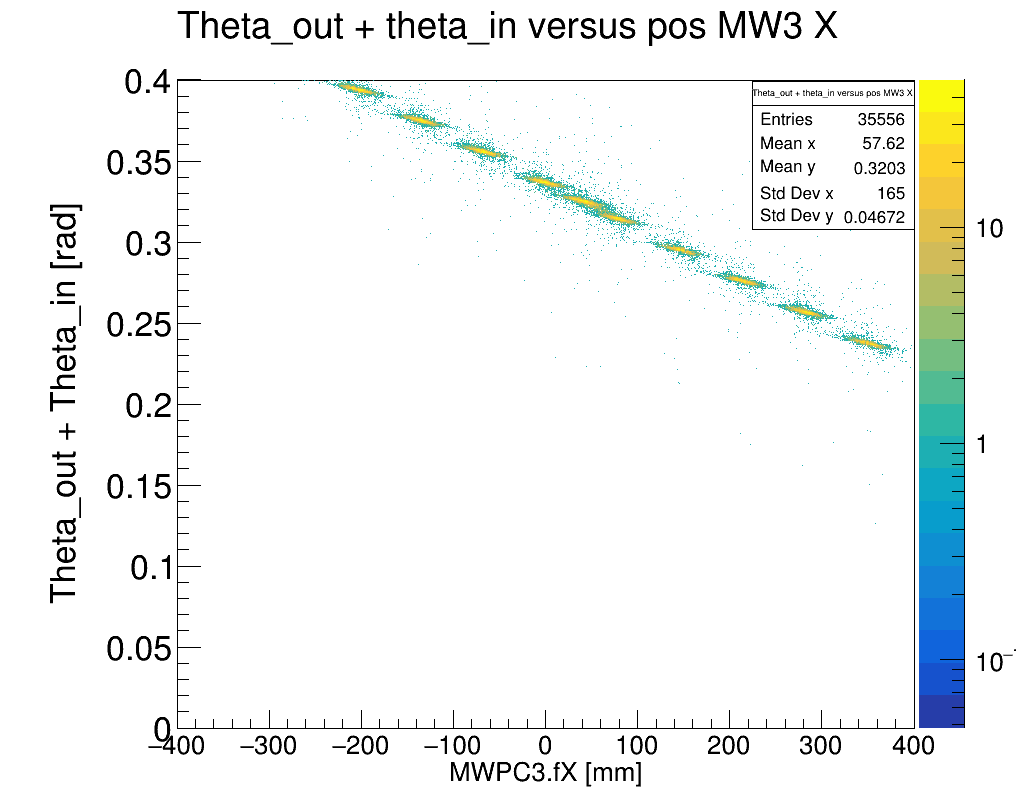
\includegraphics[width=.9\linewidth]{plot_imgs/theta_out_theta_in_mw3_corr.png} 
  \caption{"Theta \textunderscore in correction-Method"}
  \label{fig:sub-second}
\end{subfigure}
\begin{subfigure}{.5\textwidth}
  \centering
  % include second image
  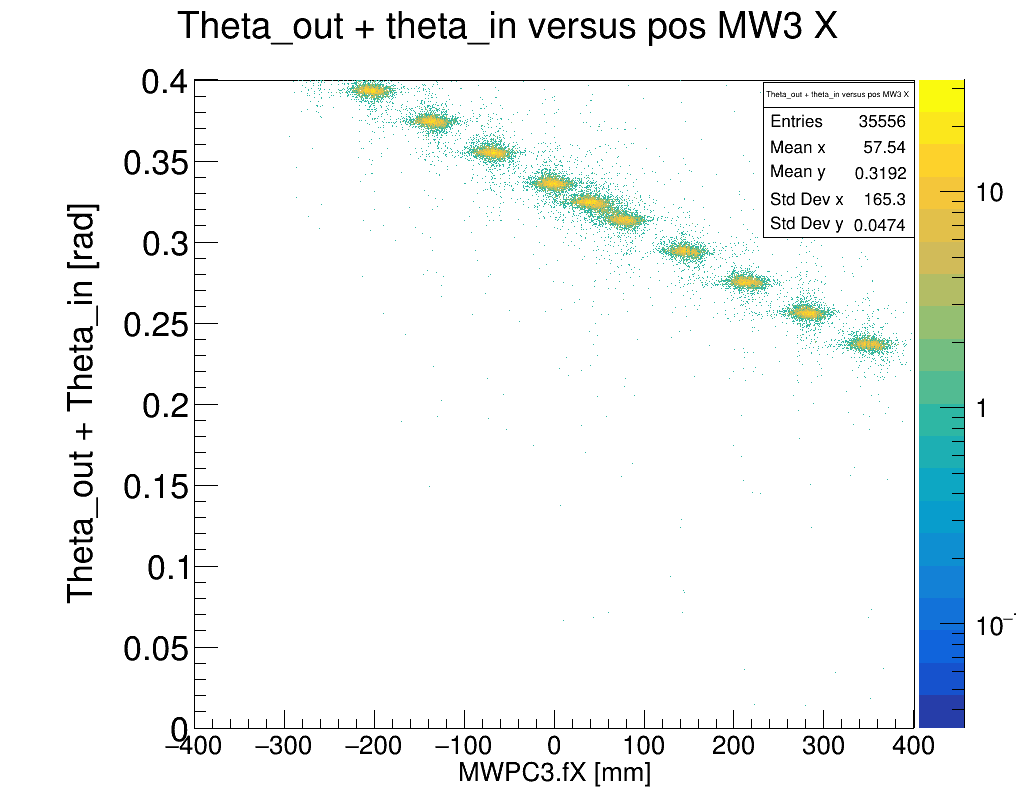
\includegraphics[width=.9\linewidth]{plot_imgs/theta_out_theta_in_mw3_fit.png} 
  \caption{"Fit-Track-Method"}
  \label{fig:sub-second}
\end{subfigure}
\begin{subfigure}{.5\textwidth}
  \centering
  % include second image
  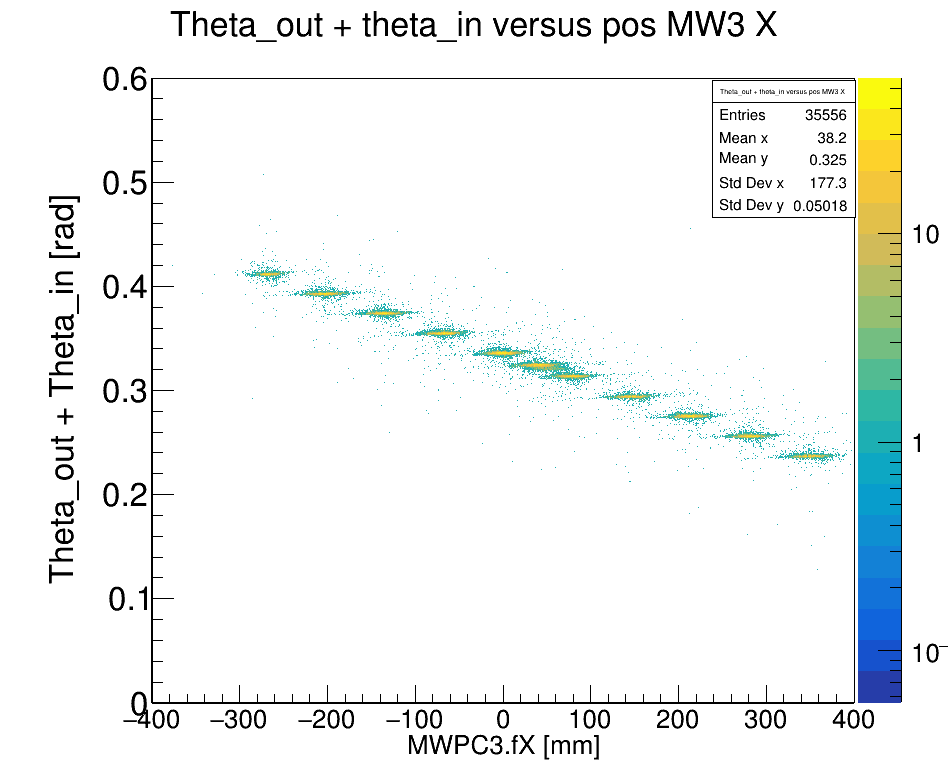
\includegraphics[width=.9\linewidth]{plot_imgs/theta_out_theta_in_mw3_alpha.png} 
  \caption{"Advanced Fit-Track-Method"}
  \label{fig:sub-second}
\end{subfigure}
\caption{Theta \textunderscore out + theta \textunderscore in vs MWPC3 x position for sweep runs 39-61.}
\label{fig:fig}
\end{figure}
\FloatBarrier
\clearpage
\subsection{theta\textunderscore in vs Radius}
\begin{figure}[!htbp]
\begin{subfigure}{.5\textwidth}
  \centering
  % include first image
  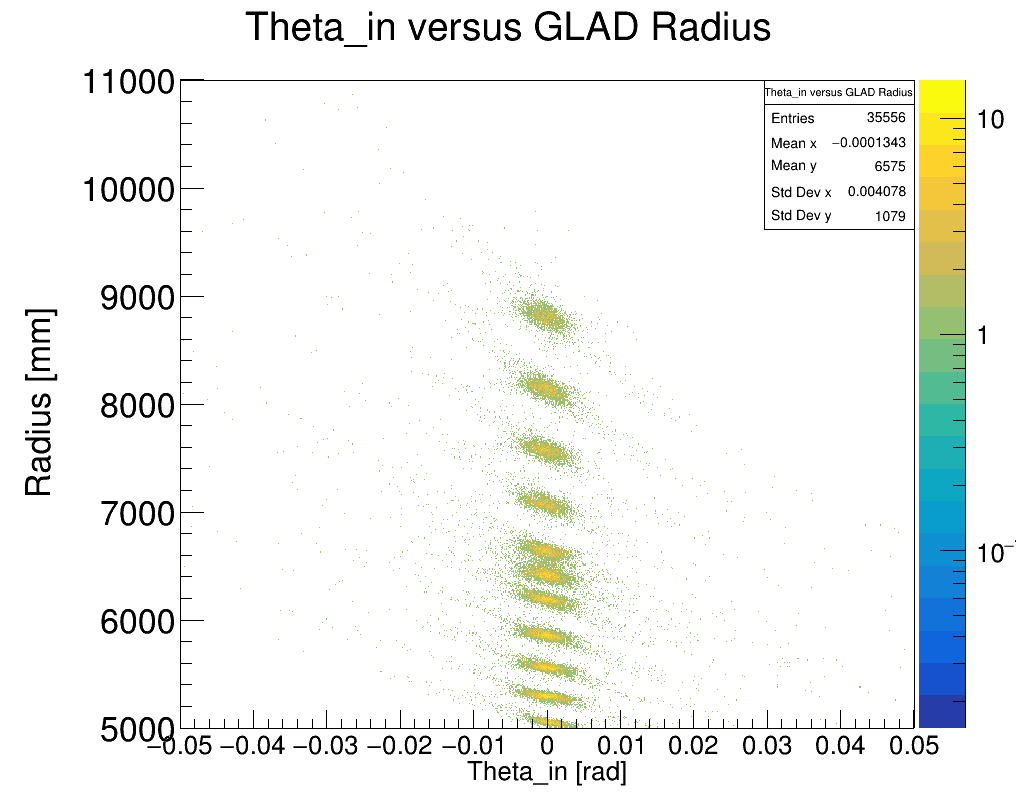
\includegraphics[width=.9\linewidth]{plot_imgs/theta_in_rho_get_centr.png}  
  \caption{"Kickplane-Method"}
  \label{fig:sub-first}
\end{subfigure}
\begin{subfigure}{.5\textwidth}
  \centering
  % include second image
  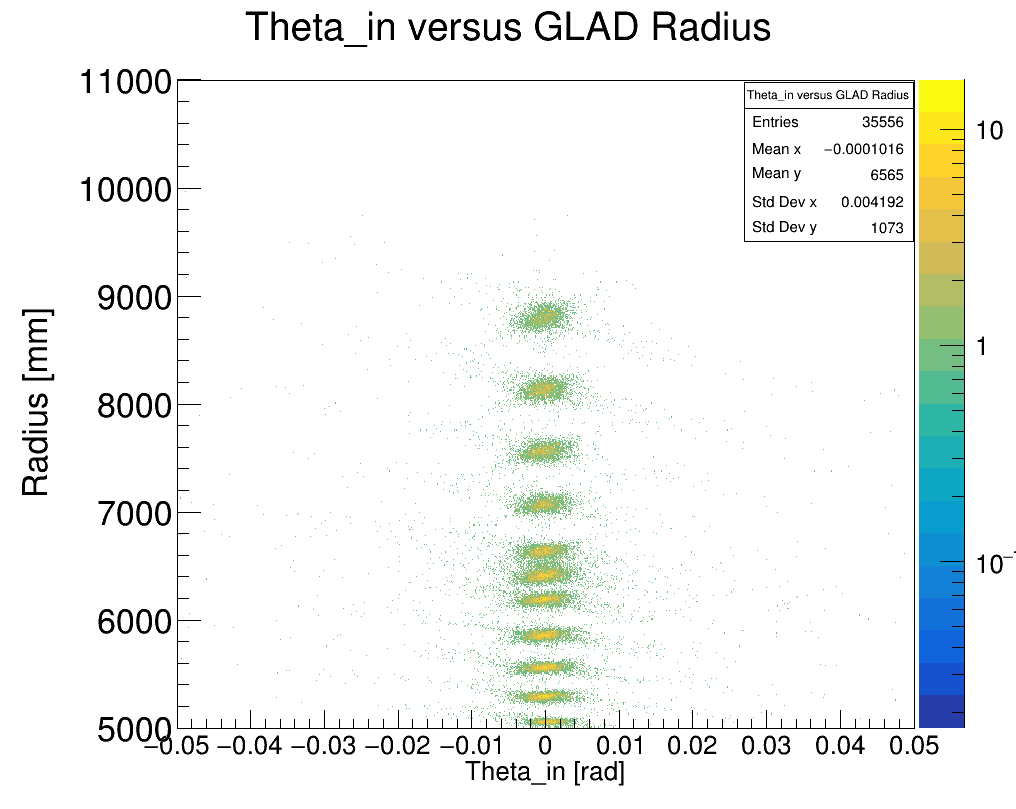
\includegraphics[width=.9\linewidth]{plot_imgs/theta_in_rho_corr.png} 
  \caption{"Theta \textunderscore in correction-Method"}
  \label{fig:sub-second}
\end{subfigure}
\begin{subfigure}{.5\textwidth}
  \centering
  % include second image
  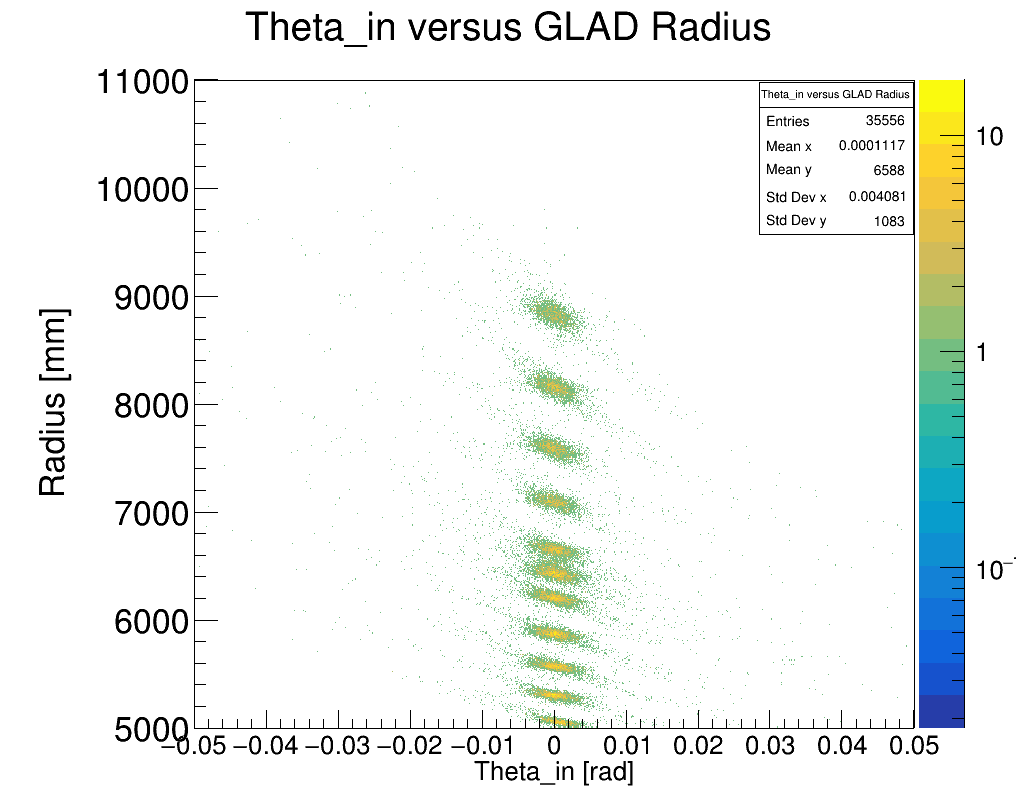
\includegraphics[width=.9\linewidth]{plot_imgs/theta_in_rho_fit.png} 
  \caption{"Fit-Track-Method"}
  \label{fig:sub-second}
\end{subfigure}
\begin{subfigure}{.5\textwidth}
  \centering
  % include second image
  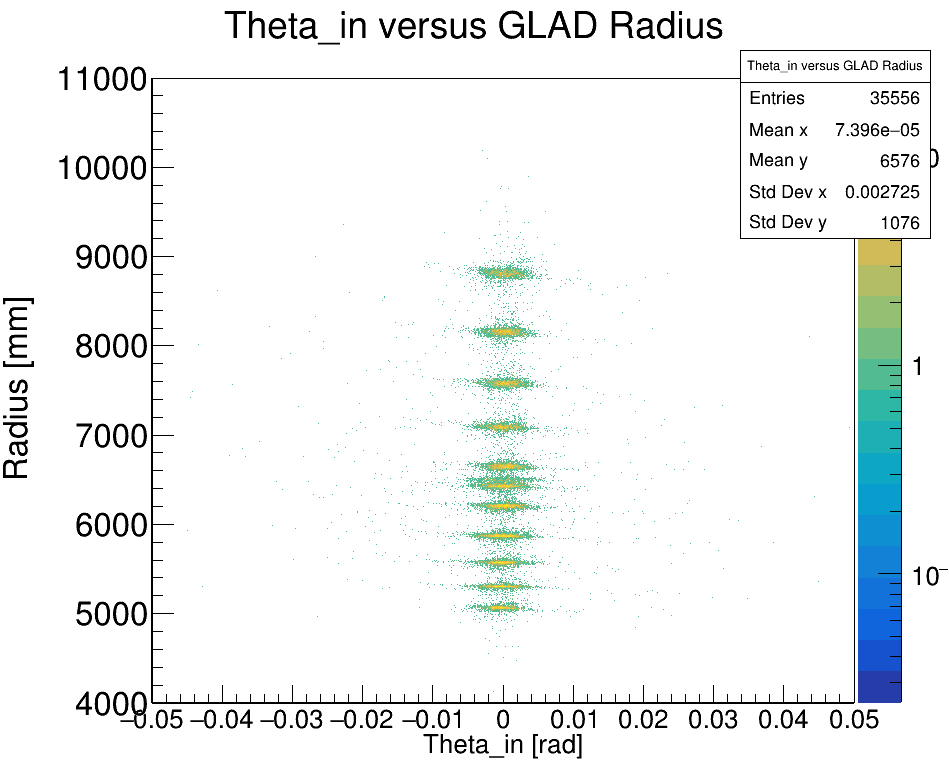
\includegraphics[width=.9\linewidth]{plot_imgs/theta_in_rho_alpha.png} 
  \caption{"Advanced Fit-Track-Method"}
  \label{fig:sub-second}
\end{subfigure}
\caption{Theta \textunderscore in vs GLAD Radius for sweep runs 39-61.}
\label{fig:fig}
\end{figure}
\FloatBarrier
\clearpage
\subsection{theta\textunderscore out vs Radius}
\begin{figure}[!htbp]
\begin{subfigure}{.5\textwidth}
  \centering
  % include first image
  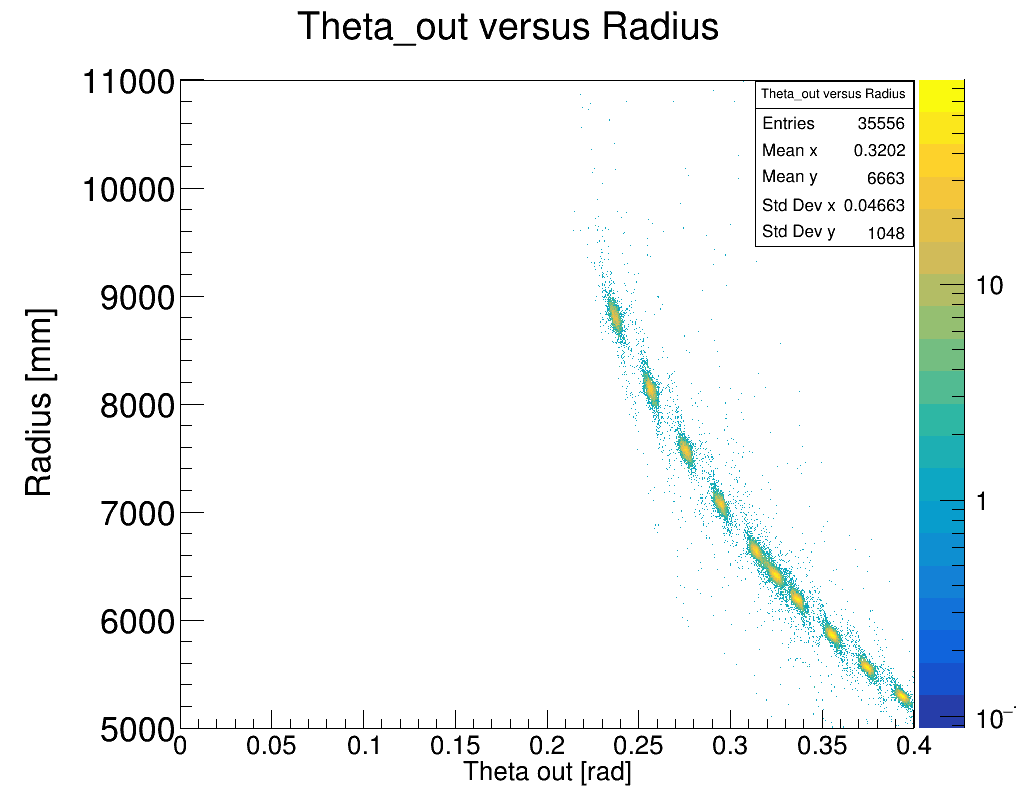
\includegraphics[width=.9\linewidth]{plot_imgs/theta_out_rho_get_centr.png}  
  \caption{"Kickplane-Method"}
  \label{fig:sub-first}
\end{subfigure}
\begin{subfigure}{.5\textwidth}
  \centering
  % include second image
  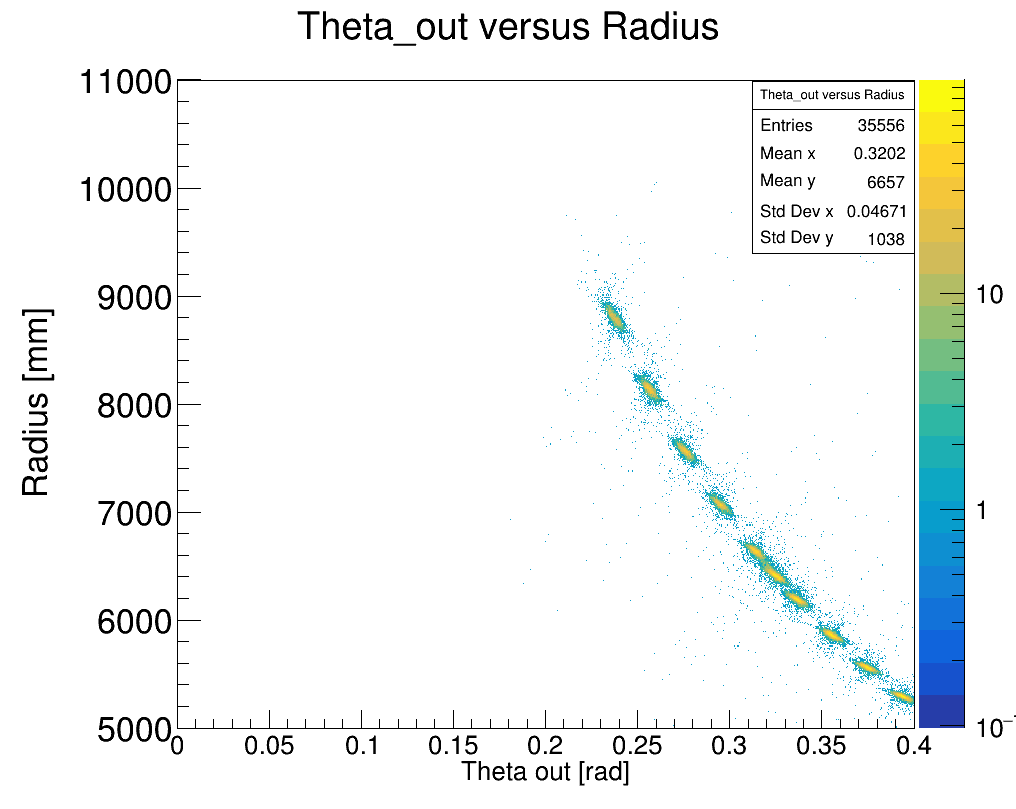
\includegraphics[width=.9\linewidth]{plot_imgs/theta_out_rho_corr.png} 
  \caption{"Theta \textunderscore in correction-Method"}
  \label{fig:sub-second}
\end{subfigure}
\begin{subfigure}{.5\textwidth}
  \centering
  % include second image
  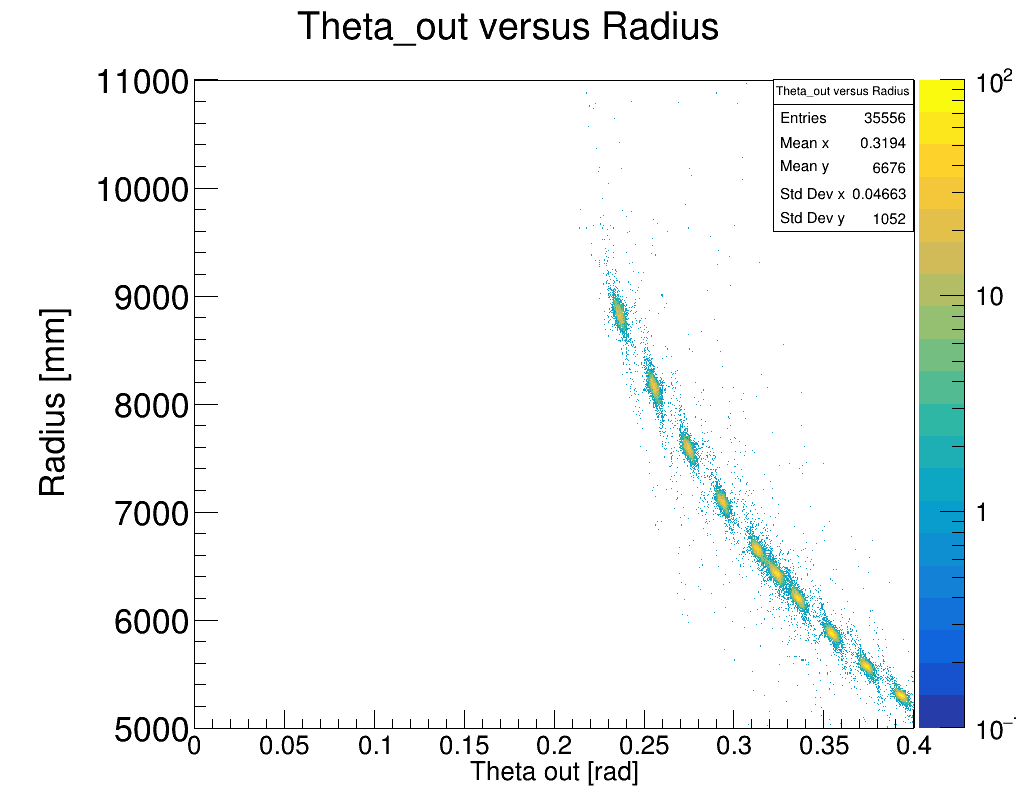
\includegraphics[width=.9\linewidth]{plot_imgs/theta_out_rho_fit.png} 
  \caption{"Fit-Track-Method"}
  \label{fig:sub-second}
\end{subfigure}
\begin{subfigure}{.5\textwidth}
  \centering
  % include second image
  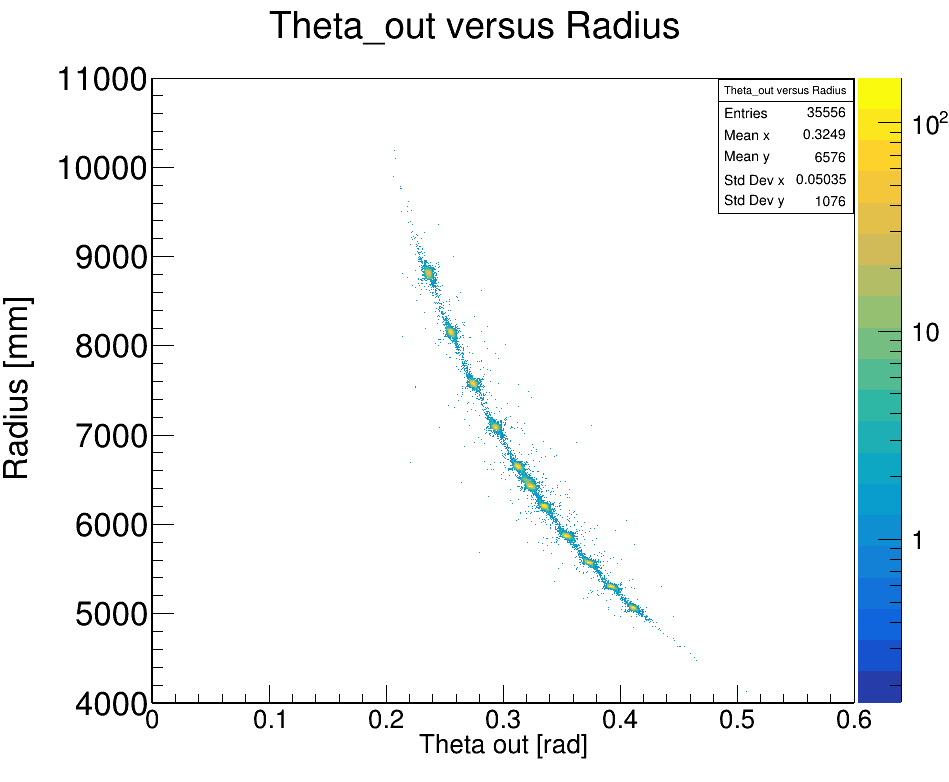
\includegraphics[width=.9\linewidth]{plot_imgs/theta_out_rho_alpha.png} 
  \caption{"Advanced Fit-Track-Method"}
  \label{fig:sub-second}
\end{subfigure}
\caption{Theta \textunderscore out vs GLAD Radius for sweep runs 39-61.}
\label{fig:fig}
\end{figure}
\FloatBarrier
\clearpage
\subsection{theta\textunderscore in vs theta\textunderscore out}
\begin{figure}[!htbp]
\begin{subfigure}{.5\textwidth}
  \centering
  % include first image
  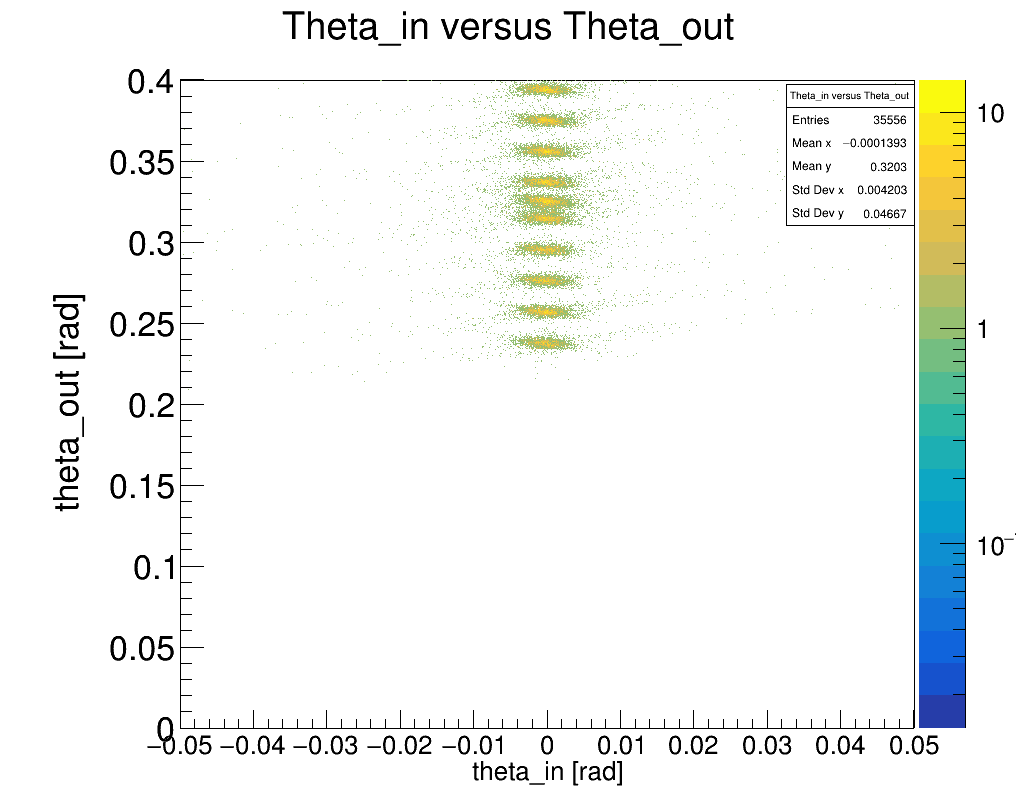
\includegraphics[width=.9\linewidth]{plot_imgs/theta_in_theta_out_get_centr.png}  
  \caption{"Kickplane-Method"}
  \label{fig:sub-first}
\end{subfigure}
\begin{subfigure}{.5\textwidth}
  \centering
  % include second image
  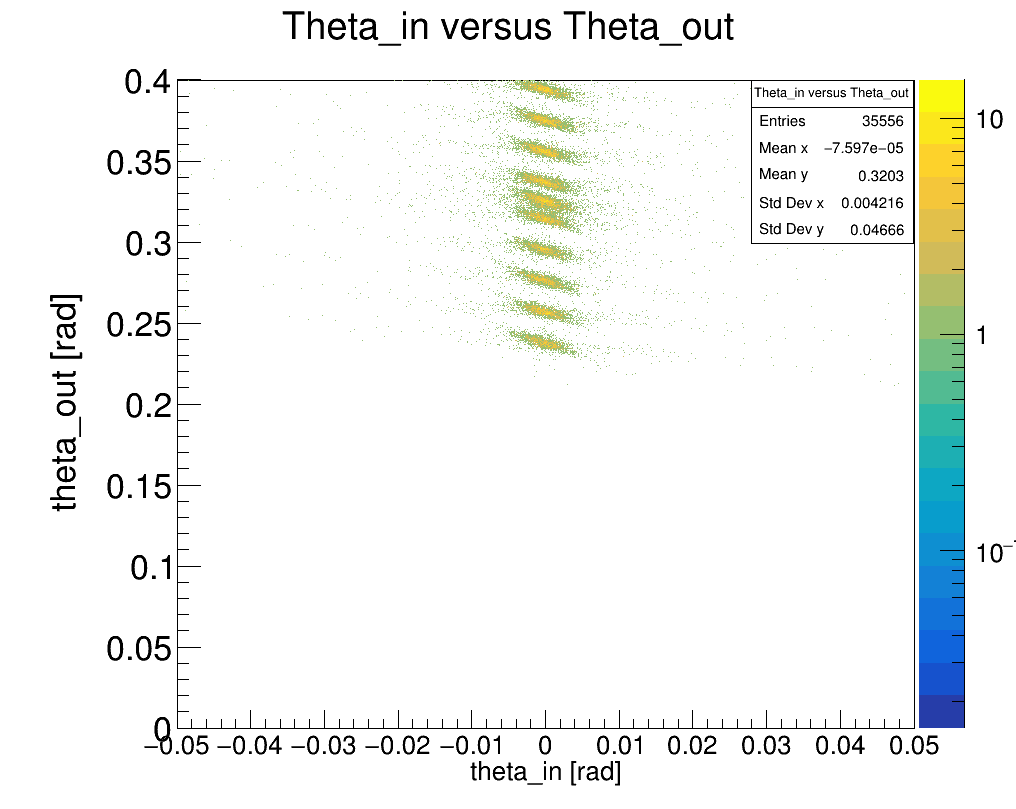
\includegraphics[width=.9\linewidth]{plot_imgs/theta_in_theta_out_corr.png} 
  \caption{"Theta \textunderscore in correction-Method"}
  \label{fig:sub-second}
\end{subfigure}
\begin{subfigure}{.5\textwidth}
  \centering
  % include second image
  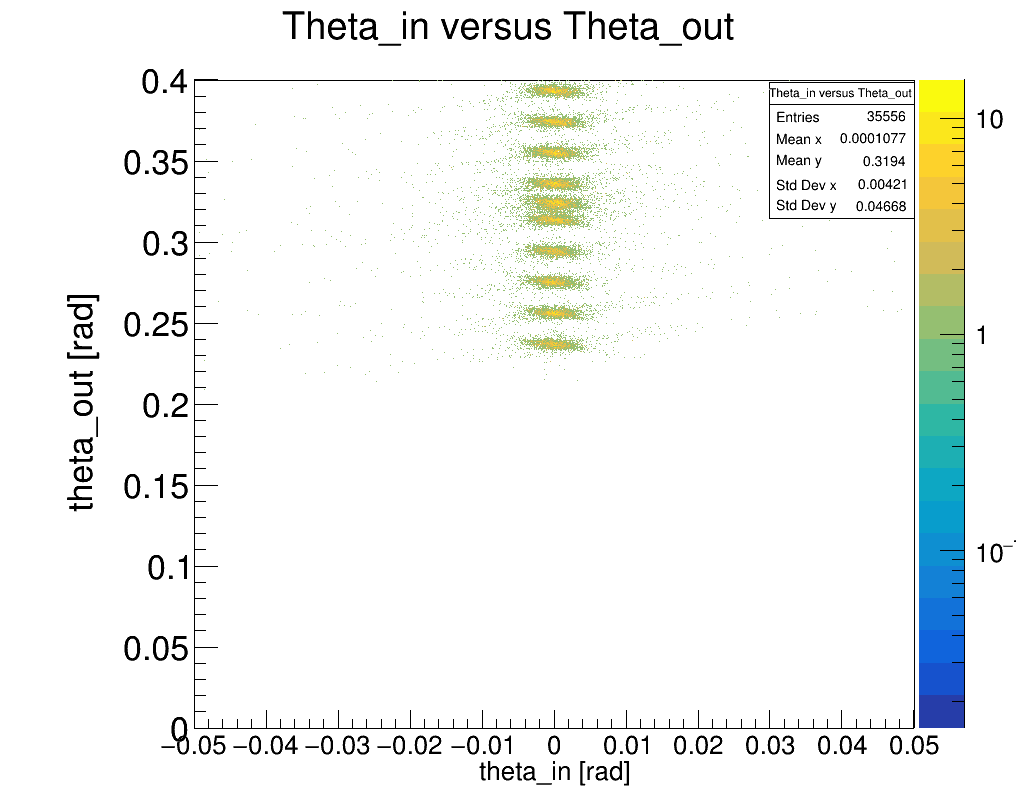
\includegraphics[width=.9\linewidth]{plot_imgs/theta_in_theta_out_fit.png} 
  \caption{"Fit-Track-Method"}
  \label{fig:sub-second}
\end{subfigure}
\begin{subfigure}{.5\textwidth}
  \centering
  % include second image
  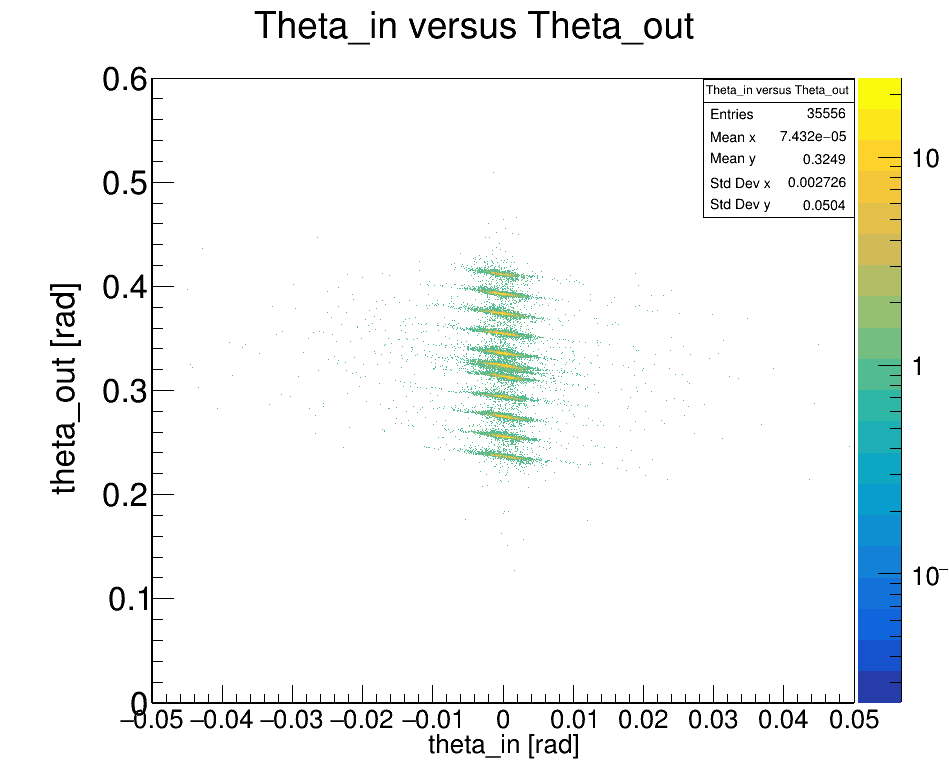
\includegraphics[width=.9\linewidth]{plot_imgs/theta_in_theta_out_alpha.png} 
  \caption{"Advanced Fit-Track-Method"}
  \label{fig:sub-second}
\end{subfigure}
\caption{Theta \textunderscore in vs theta \textunderscore out for sweep runs 39-61.}
\label{fig:fig}
\end{figure}
\FloatBarrier
\clearpage
\subsection{MW3 vs Radius - x position}
\begin{figure}[!htbp]
\begin{subfigure}{.5\textwidth}
  \centering
  % include first image
  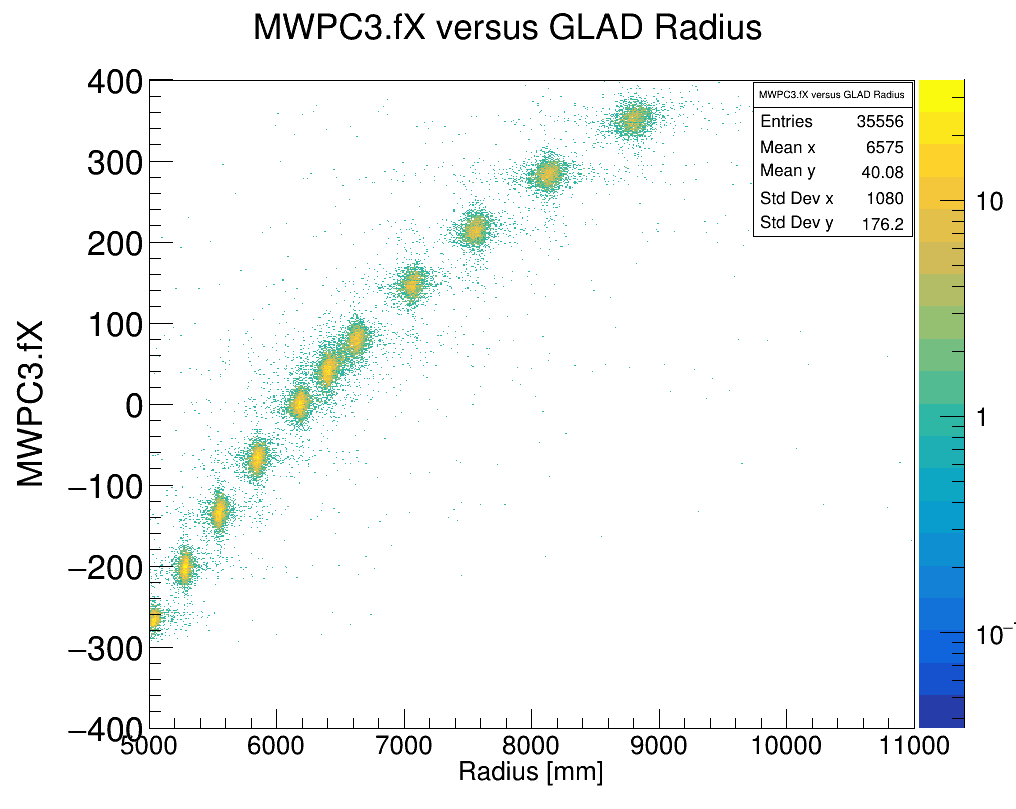
\includegraphics[width=.9\linewidth]{plot_imgs/mw3_rho_get_centr.png}  
  \caption{"Kickplane-Method"}
  \label{fig:sub-first}
\end{subfigure}
\begin{subfigure}{.5\textwidth}
  \centering
  % include second image
  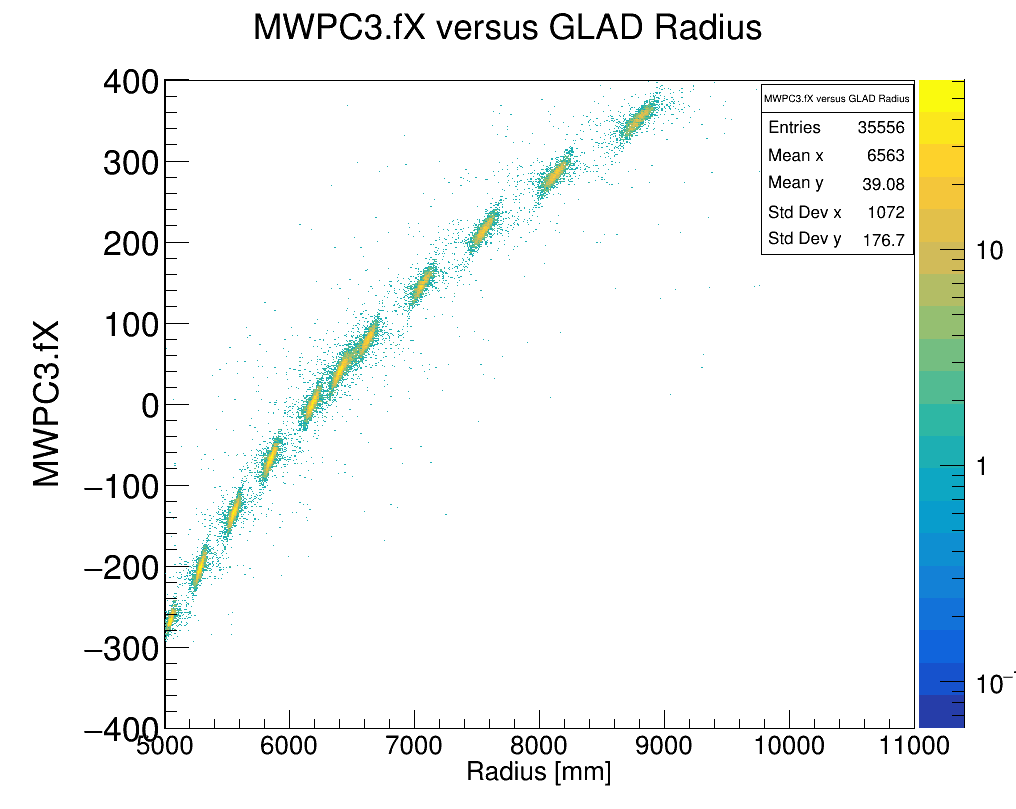
\includegraphics[width=.9\linewidth]{plot_imgs/mw3_rho_corr.png} 
  \caption{"Theta \textunderscore in correction-Method"}
  \label{fig:sub-second}
\end{subfigure}
\begin{subfigure}{.5\textwidth}
  \centering
  % include second image
  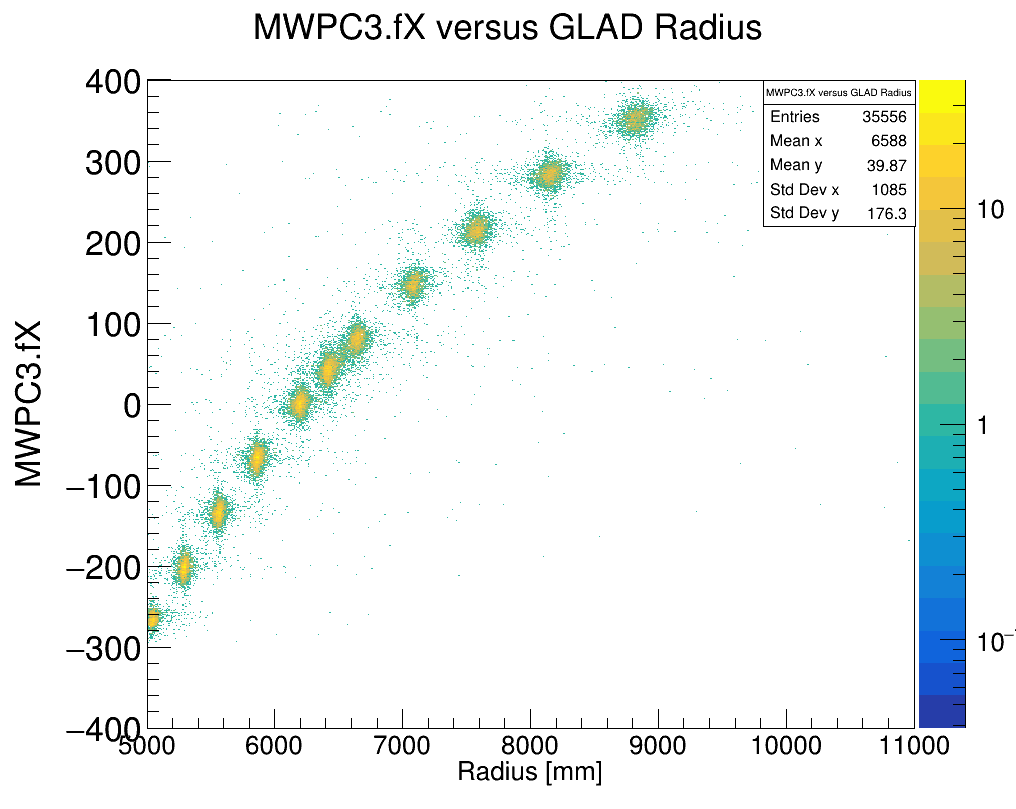
\includegraphics[width=.9\linewidth]{plot_imgs/mw3_rho_fit.png} 
  \caption{"Fit-Track-Method"}
  \label{fig:sub-second}
\end{subfigure}
\begin{subfigure}{.5\textwidth}
  \centering
  % include second image
  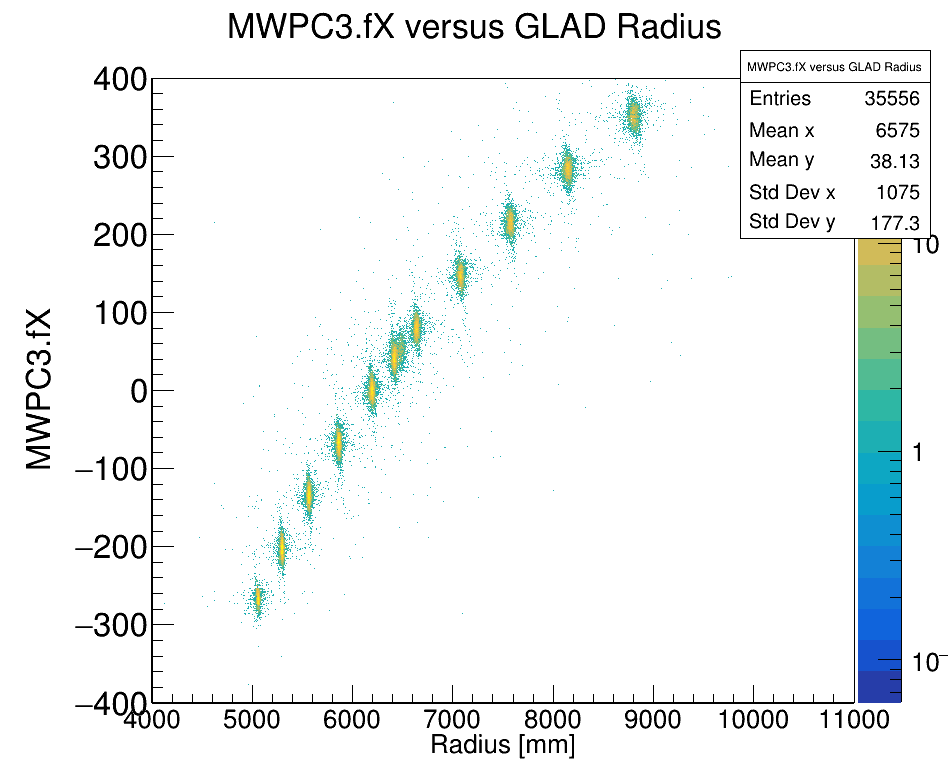
\includegraphics[width=.9\linewidth]{plot_imgs/mw3_rho_alpha.png} 
  \caption{"Advanced Fit-Track-Method"}
  \label{fig:sub-second}
\end{subfigure}
\caption{MWPC3 x position vs GLAD Radius for sweep runs 39-61.}
\label{fig:fig}
\end{figure}
\FloatBarrier
\clearpage
\subsection{MW2 vs Radius - x position}
\begin{figure}[!htbp]
\begin{subfigure}{.5\textwidth}
  \centering
  % include first image
  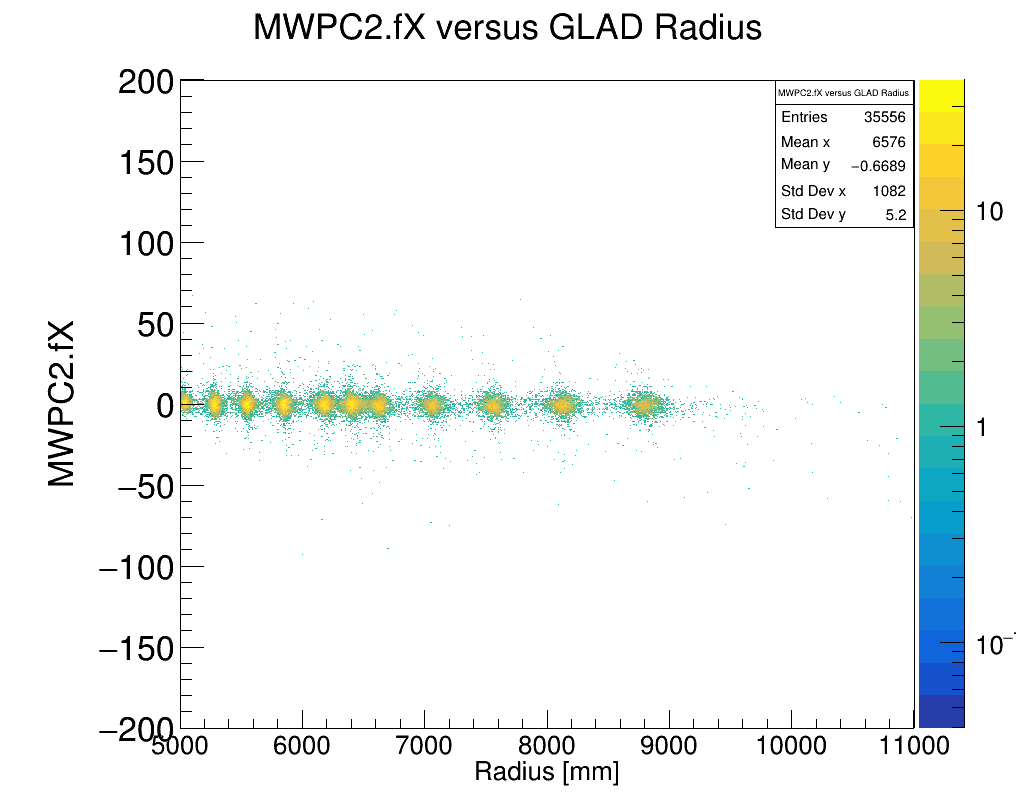
\includegraphics[width=.9\linewidth]{plot_imgs/mw2_rho_get_centr.png}  
  \caption{"Kickplane-Method"}
  \label{fig:sub-first}
\end{subfigure}
\begin{subfigure}{.5\textwidth}
  \centering
  % include second image
  \includegraphics[width=.9\linewidth]{plot_imgs/mw2_rho_corr.png} 
  \caption{"Theta \textunderscore in correction-Method"}
  \label{fig:sub-second}
\end{subfigure}
\begin{subfigure}{.5\textwidth}
  \centering
  % include second image
  \includegraphics[width=.9\linewidth]{plot_imgs/mw2_rho_fit.png} 
  \caption{"Fit-Track-Method"}
  \label{fig:sub-second}
\end{subfigure}
\begin{subfigure}{.5\textwidth}
  \centering
  % include second image
  \includegraphics[width=.9\linewidth]{plot_imgs/mw2_rho_alpha.png} 
  \caption{"Advanced Fit-Track-Method"}
  \label{fig:sub-second}
\end{subfigure}
\caption{MWPC2 x position vs GLAD Radius for sweep runs 39-61.}
\label{fig:fig}
\end{figure}
\FloatBarrier
\clearpage

\section{Relative momentum resolution "Advanced Fit-Track-Method"}

The momentum resolution is calculated from the radius-calculation as $\rho \sim p$. From that follows:\\
\\
$\frac{\Delta p}{p} = \frac{\Delta\rho}{\rho}$
\\
\newline
For the evaluation of the resolutions for the various sweep runs the two dimensional plot "MWPC3.fX versus GLAD Radius" is projected on the abscissa. The resulting 1D plot is fitted with a gaussian. The mean value from the fit corresponds to $\rho$ and the $\sigma$ to $\Delta\rho$ respectively.\\
\\
\begin{tabular}{|c|c|c|c|}
\hline
Runnr. & $\overline{\rho}$ & $\sigma$ & rel. resolution \\
\hline
39     &      6.48911e+03       &    2.13410e+01    &     3.289e-03\\
40     &      6.42396e+03       &    1.56313e+01    &     2.433e-03\\
42     &      6.20033e+03       &    1.42716e+01    &     2.301e-03\\
44     &      5.86854e+03       &    1.29449e+01    &     2.206e-03\\
46     &      5.57125e+03       &    1.31369e+01    &     2.358e-03\\
48     &      5.30203e+03       &    1.07044e+01    &     2.018e-03\\
51     &      5.06232e+03       &    1.07182e+01    &     2.117e-03\\
53     &      6.64556e+03       &    1.66141e+01    &     2.500e-03\\
55     &      7.08710e+03       &    1.91895e+01    &     2.708e-03\\
57     &      7.57474e+03       &    2.16135e+01    &     2.853e-03\\
59     &      8.15089e+03       &    2.22151e+01    &     2.725e-03\\
61     &      8.81055e+03       &    2.72038e+01    &     3.088e-03\\

\hline

\end{tabular}
\\
\\
\newline
With mean relative resolution $\frac{\Delta\rho}{\rho}$ = 2.55e-03.





\section{Limiting Radius/Momentum resolution factors}

The radius/momentum resolution is limited by:\\
\begin{itemize}
\item Energy straggling
\item Angular straggling
\item Angular resolution of MWPC1/2
\item position resolution of MWPC3 (higher order??)
\end{itemize}

\subsection{Engergy straggling}

For the error calculation the mean energy inside the GLAD was used and the corresponding standard deviation. 
Generally for a charged particle drifting through a magnetic field the radius of the curved path the particle is following is defined as:\\
\\
$\rho = \frac{\gamma \cdot \beta \cdot m}{q \cdot B}$\\
(considering c = 1)\\
Energy straggling has an effect on $\beta$ and $\gamma$ respectively. The measurement uncertainty with respect to $\beta$ can be calculated as follows:\\
$\frac{d\rho}{d\beta} = \frac{1}{(\sqrt{1-\beta^2})^3}\cdot \frac{m}{qB}$\\
\newline
$\Delta\rho_{\beta} = \frac{d\rho}{d\beta} \cdot \Delta\beta = \frac{\Delta\beta}{(\sqrt{1-\beta^2})^3}\cdot \frac{m}{qB}$\\

with relative measurement uncertainty $\frac{\Delta\rho_{\beta}}{\rho} = 5.434e-04$\\

\subsection{Angular straggling}
For the error calculation originating from angular straggling it is considered only angular straggling starting from the backend of the MWPC1. That means for this error calculation it is assumed to have a perfect focussed beam undergoes no broadening until it hits the MWPC1 (always at the same x-y-z position). Angular straggling broadens the beam focus and affects therefore both $\Theta$\textunderscore in and $\Theta$\textunderscore out. \\
(angular straggling for $\Theta$\textunderscore in can be neglected, higher order...)\\
For the calculation of  measurement uncertainty with respect to $\Theta$\textunderscore out we use the simplified geometrical formula of the radius:\\
$\rho = \frac{L_{eff}}{2\cdot\sin(\frac{\Theta{in}+\Theta{out}}{2})}$\footnote{on the following pages I set $\Theta{in} = 0$ and $\Theta{out}$ to the value given by the GLAD field calculator(Mass = 12, Charge = 6, Energy = 400 A/MeV, Current = 1444), see \url{http://web-docs.gsi.de/~land/glad/}.}\\ 
From that follows:\\
$\Delta\rho_{\Theta{out}} = -\rho\cdot \frac{1}{2\cdot\tan(\frac{\Theta{in}+\Theta{out}}{2})}\cdot\Delta\Theta{out}$\\
with $\Delta\Theta_{out} = 3.401e-04$. This is the value calculated with LISE++ from MWPC1 to the very center of GLAD. 
Hence:\\
$\Big|\frac{\Delta\rho{\Theta{out}}}{\rho}\Big| = \frac{1}{2\cdot\tan(\frac{\Theta{in}+\Theta{out}}{2})}\cdot\Delta\Theta{out} = $1.079e-03

\subsection{Angular resolution of MWPC1/2}
$\Delta\rho_{\Theta{in}} = -\rho\cdot \frac{1}{2\cdot\tan(\frac{\Theta{in}+\Theta{out}}{2})}\cdot\Delta\Theta{in}$ \\
with $\Delta\Theta_{in} = \frac{2\cdot \Delta x}{L} $\footnote{$\Theta_{in} = \frac{x_{2}-x{1}}{L}$, $\Delta\Theta_{in} = \big|\frac{d\Theta_{in}}{dx_{2}} \big|\cdot \Delta x_{2} + \big|\frac{d\Theta_{in}}{dx_{1}} \big|\cdot \Delta x_{1} = \frac{2\cdot \Delta x}{L}$} and L the (z-)distance between MWPC1 and MWPC2 (= 575mm).\\
\newline
With $\Delta x = 0.1mm$ it follows:\\
\newline
$\Big|\frac{\Delta\rho_{\Theta_{in}}}{\rho}\Big| = $ 1.104e-03.
\newline
\newline
Adding up the above errors quadratically we get:\\
$\Big|\frac{\Delta\rho}{\rho}\Big| = \sqrt{(5.434\cdot10^{-4})^{2}+(1.079\cdot10^{-3})^{2}+(1.104\cdot10^{-3})^{2}} = 1.64\cdot10^{-3} $

\subsection{Limiting Radius resolution factors on data}
For this subsection RUN 53 (with GLAD current = 1444A) is taken in account.\\
From the table of relative radius resolution we see that for RUN 53 it corresponds to 2.500e-03. The contribution from angular resolution of MWPC1/2 is 1.104e-03 (see previous section). The major limiting factor, the angular straggling can be retrieved from the resolution of theta \textunderscore out. It has to be considered that the resolution of theta \textunderscore out is affected by the beam broadening before the MWPC1. To account for that it has to be analyzed the impact of theta \textunderscore in on theta \textunderscore out. \\
Therefore an offset of 1 mrad is added to  theta \textunderscore in and the mean values for theta \textunderscore out can be compared :\\
\begin{itemize}
\item theta \textunderscore out without shift: $3.13257\cdot10^{-1}$
\item theta \textunderscore out with 1 mrad theta \textunderscore in shift: $3.13912\cdot10^{-1}$
\item difference: $6.55\cdot10^{-1}$mrad
\end{itemize}
That means we have a translation factor (for small angles) of 0.655 for theta \textunderscore in to theta \textunderscore out.\\
The error calculation in the previous section predicts following angular straggling error:\\
$2.5\cdot10^{-3} = \sqrt{(1.104\cdot10^{-3})^{2}+(\Big|\frac{\Delta\rho{\Theta_{out}}}{\rho}\Big|)^{2}}$ \\
follows:\\
$\Big|\frac{\Delta\rho{\Theta_{out}}}{\rho}\Big| = 2.24\cdot10^{-3}$\\
$\Longrightarrow 2.24\cdot10^{-3} \cdot \tan(0.15625) \cdot 2 = 7.1 \cdot 10^{-4} =  \Delta\theta_{out}$ \\
The angular resolution of theta \textunderscore out from data is 1.78045E-03. From this value the angular beam broadening (multiplied by the translation factor) before MWPC1 has to be substracted:\\
$\Delta\theta_{out} = 1.78045\cdot10^{-3} -0.655 \cdot 1.61086\cdot 10^{-3} = 7.253 \cdot 10^{-4} $\\
This result coincides well with the predicted one and confirms that the predominant factors for the limiting radius resolution are angular straggling and the angular resolution of MWPC1/2.



\section{Scalability of the field}
Using the sweep runs (39-61) with different GLAD currents, the scalability of the B-Field can be analyzed. In figure \ref{fig:scalar} B\textunderscore$\rho$  from GLAD calculator divided by the mean radius is plotted against the according current values.\\ 
 \begin{figure}[!htb]
	\includegraphics[width=0.8\textwidth]{scalar.png}
	\caption{\label{fig:scalar}}
	\label{fig:scalar}
\end{figure}
Taking the assumption that:\\
$B = current \cdot k $ (with k being a constant)\\
we get from the fit in \ref{fig:scalar}:\\
slope = 0.000610713 \\
offset = 0.0709244\\
When plotting the proprotional factor $k$ (which is equal to $\frac{Brho}{I\rho}$, with $Brho$ from GLAD calculator and $\rho$ equal to the mean radius for each run) for each RUN versus the current and adding the proprotional factor from the fit as a straight line, we can see in figure \ref{fig:factor_k} that the factor $k$ from the fit seems to be slightly underestimated. \\
\begin{figure}[!htb]
	\includegraphics[width=0.8\textwidth]{curent_vs_k_factor.png}
	\caption{\label{fig:factor_k}}
	\label{fig:factor_k}
\end{figure}

\section{Z versus A/q calculations}
In this section the target RUNs 82,83,86,88 are analyzed with GLAD current = 1444 A, target = CH2 12.29 mm.\\
Data is taken for the x-position on MW1,MW2 and MW3, time difference between START and TOFW Detector and charge value from TWIM Music.\\
The radius of curvature in GLAD is computed using the "Advanced Fit Track" method. The time of flight is calculated using the time difference between START and TOFW with the respective offsets (for the TOF detector pads) and substracting from that the fime of flight between START detector and target. The latter is calculated using $\beta = 0.714549 (\equiv 400 A/MeV)$ and as distance between START and target  1183.25 mm.\\
\newline
Offsets used for RUNs 82 and 83 ( using sweep RUNs 39-61) and for RUNs 86 and 88 (using sweep run 36), respectively:\\
\begin{tabular}{|c|c|c|c|}
\hline
Detnr. TOFW & Time offset 39-61 [s] & Time offset 36 [s] & Difference [s] \\
\hline
1      &	1.15079E-07 &	1.141E-07    &  -9.789E-10\\
2	   &	1.13720E-07	&	1.13329E-07  &  -3.910E-10\\
3	   &	1.16304E-07	&	1.15778E-07  &  -5.259E-10\\
4 	   &	1.14539E-07	&	1.13983E-07  &  -5.560E-10\\
5	   &	1.15420E-07	&	1.14922E-07  &  -4.979E-10\\
6	   &	1.16052E-07	&	1.15593E-07  &  -4.590E-10\\
7	   &	1.16903E-07	&   1.16486E-07  &  -4.169E-10\\
8	   &	1.16143E-07	&   1.15781E-07  &  -3.620E-10\\
9	   &	1.14394E-07	&   1.14067E-07  &  -3.270E-10\\
10	   &	1.15967E-07	&   1.15691E-07  &  -2.759E-10\\
11     & 	1.12559E-07	&   1.12337E-07  &  -2.220E-10\\
12     &	1.15962E-07	&   1.15764E-07  &  -1.979E-10\\
13     &	1.13521E-07	&   1.13372E-07  &  -1.489E-10\\
14     &	1.15088E-07	&   1.14989E-07  &  -9.900E-11\\
15	   &	1.13676E-07	&   1.18635E-07  &  4.958E-09\\
16	   &	1.12992E-07	&   1.17986E-07  &  4.993E-09\\
17	   &	1.14391E-07	&   1.19424E-07  &  5.033E-09\\
18	   &	1.12076E-07	&   1.17168E-07  &  5.091E-09\\
19	   &	1.13234E-07	&   1.18360E-07  &  5.126E-09\\
20	   &	1.12760E-07	&   1.17933E-07  &  5.173E-09\\
21	   &	1.16445E-07	&   1.21687E-07  &  5.242E-09\\
22	   &	1.16877E-07	&   1.22138E-07  &  5.261E-09\\
23	   &	1.16077E-07	&   1.21353E-07  &  5.275E-09\\
24     &	1.16127E-07	&   1.21457E-07  &  5.329E-09\\
25	   &	1.14855E-07	&   1.20219E-07  &  5.363E-09\\
26	   &	1.14363E-07	&   1.19841E-07  &  5.477E-09\\
27	   &	1.14435E-07	&   1.19932E-07  &  5.496E-09\\


\hline

\end{tabular}
\newline

The proceeding for the Z versus A/q calculations are:
\begin{enumerate}
\item Plot without any cuts/restrictions Z versus Radius using the "Fit-Track" method (see \ref{fig:isotopes} ).
\item From that plot identify the various isotopes and cut on them. 
\item Plot for each isotope theta\textunderscore out vs x\textunderscore 3 and make a linear fit (see \ref{fig:iso_fit}).
\item Feed the "Advanced Fit-Track" method with the parameters of the fit for the various isotopes (which you can separate using the previously selected cuts).
\item Calculate beta (using the above TOFW offsets) for the various isotopes and plot Z versus A/q. 
\\ 
\end{enumerate}
\begin{figure}[!htb]
	\centering
	\includegraphics[width=0.7\textwidth]{isotope_separation.png}
	\caption{Z versus Radius for RUN 88.}
	\label{fig:isotopes}
\end{figure}

\begin{figure}[!htbp]
\begin{subfigure}{.5\textwidth}
  \centering
  % include first image
  \includegraphics[width=.9\linewidth]{theta_out_fit10B.png}  
  \caption{theta\textunderscore out vs xMW3 for 10B.}
  \label{fig:sub-first}
\end{subfigure}
\begin{subfigure}{.5\textwidth}
  \centering
  % include second image
  \includegraphics[width=.9\linewidth]{theta_out_fit11B.png} 
  \caption{theta\textunderscore out vs xMW3 for 11B.}
  \label{fig:sub-second}
\end{subfigure}
\begin{subfigure}{.5\textwidth}
  \centering
  % include second image
  \includegraphics[width=.9\linewidth]{theta_out_fit11C.png} 
  \caption{theta\textunderscore out vs xMW3 for 11C.}
  \label{fig:sub-second}
\end{subfigure}
\begin{subfigure}{.5\textwidth}
  \centering
  % include second image
  \includegraphics[width=.9\linewidth]{theta_out_fit12C.png} 
  \caption{theta\textunderscore out vs xMW3 for 12C.}
  \label{fig:sub-second}
\end{subfigure}
\caption{theta\textunderscore out vs xMW3 for isotopes.}
\label{fig:iso_fit}
\end{figure}


The cuts on the various isotopes in \ref{fig:isotopes} are:\\
10B: $4 < Z < 5.4 $ and $6266 < \rho < 6735$\\
11B: $4 < Z < 5.5$ and $6888 < \rho < 7363$\\
11C: $5.2 < Z < 6.8$ and $5774 < \rho < 6189$\\
12C: $5.4 < Z < 6.8$ and $6295 < \rho < 6768$\\
\newline
Using this cuts we get following fit parameters for the various isotopes:\\
\newline
\begin{tabular}{|c|c|c|c|}
\hline
Isotope & $\alpha$ & a (= slope) & b (=offset) \\
\hline
\textbf{10B:} & 0.32 & 0.000144005 & 0.327681\\
\hline
\textbf{11B:} & 0.2932 & 0.000139928 & 0.313335\\
\hline
\textbf{11C:} & 0.348 & 0.000146679 & 0.34352\\
\hline
\textbf{12C:} & 0.3179 & 0.00014353 & 0.326665\\
\hline
\end{tabular}
\\
\newline
Separating the isotopes by the above charge and radius cuts and using the appropriate $\alpha$, a and b parameters the Radius gets recalculated via the "Advanced Fit-Track" method. The new value for the radius is now used in the A/q calculation:\\
A/q = $\frac{B \cdot \rho \cdot e}{\gamma\cdot\beta \cdot c \cdot u}$ \\
with:\\
$e$: elementary charge = $1.602176634\cdot10^{-19}$C\\
$c$: speed of light = 299792458 m/s\\
$u$: atomic mass unit = $1.66053906660\cdot10^{-27}$kg\\
In figure \ref{fig:z_vs_aq} the separated isotopes are shown.
\begin{figure}[!htb]
	\centering
	\includegraphics[width=0.7\textwidth]{z_vs_aq_combined.png}
	\caption{Z versus A/q for run 88 with target CH2 12.29 mm.}
	\label{fig:z_vs_aq}
\end{figure}

\begin{figure}[!htbp]
\begin{subfigure}{.5\textwidth}
  \centering
  % include first image
  \includegraphics[width=.9\linewidth]{z_vs_aq_12c.png}  
  \caption{$5.4 < q < 6.8$; $6295 < \rho < 6768$}
  \label{fig:sub-first}
\end{subfigure}
\begin{subfigure}{.5\textwidth}
  \centering
  % include second image
  \includegraphics[width=.9\linewidth]{z_vs_aq_11c.png} 
  \caption{$5.2 < q < 6.8$; $ 5774 < \rho < 6189$}
  \label{fig:sub-second}
\end{subfigure}
\begin{subfigure}{.5\textwidth}
  \centering
  % include second image
  \includegraphics[width=.9\linewidth]{z_vs_aq_11b.png} 
  \caption{$4 < q < 5.5$; $6888 < \rho < 7363$}
  \label{fig:sub-second}
\end{subfigure}
\begin{subfigure}{.5\textwidth}
  \centering
  % include second image
  \includegraphics[width=.9\linewidth]{z_vs_aq_10b.png} 
  \caption{$4 < q < 5.4$; $ 6266 < \rho < 6735$}
  \label{fig:sub-second}
\end{subfigure}
\caption{Z versus A/q for runs 82, 83, 86, 88 with target CH2 12.29 mm.}
\label{fig:iso_fit}
\end{figure}


\subsection{Limiting Mass number resolution factors\footnote{This analysis was done with RUN 88, CH2 target, 12.29mm, GLAD current = 1444 A on the isotope 12C}}

From the formula:\\
A/q = $\frac{B \cdot \rho \cdot e}{\gamma\cdot\beta \cdot c \cdot u}$ \\
we can see that the determination of A/q is limited by the radius $\rho$ and time measurement and path calculation .\\
That means:\\
\newline
$\Big|\frac{\Delta A/q}{A/q}\Big| = \sqrt{\big|\frac{\Delta A/q_{\rho}}{A/q}\big|^{2} + \big|\frac{\Delta A/q_{t}}{A/q}\big|^{2} +\big|\frac{\Delta A/q_{s}}{A/q} \big|^{2}  }$ \\
with:\\
$\big|\frac{\Delta A/q_{\rho}}{A/q}\big| = \big|\frac{\Delta\rho}{\rho}\big|$\\
and\\
$\big|\frac{\Delta A/q_{t}}{A/q}\big| = \frac{\Delta t}{t\cdot(1-\beta^{2})}$ \footnote{$d\beta = -\frac{s}{c\cdot t^{2}}\Delta t = -\frac{\beta \cdot \Delta t}{t}$;\hspace{1cm}$\frac{dA/q}{d\beta} = -B\cdot\rho\cdot\frac{1}{\beta^{2}\cdot\sqrt{1-\beta^{2}}}\Delta\beta = \frac{B\cdot \rho}{\beta \cdot t \cdot \sqrt{1-\beta^{2}}}\cdot \Delta t$}\\
$\Delta t$ corresponds to the resolution of the time measurement of the TOFW.\\
As we do not just measure the time of flight in the presence of the magnetic field of GLAD, but the entire flightpath, we use for $t$ the time of flight from target to the ToFW and as $s$ the calculated pathlength. \\
$t = \frac{s}{\beta\cdot c} =  \frac{7.547m}{0.714549\cdot c} = 3.54\cdot10^{-8}s$\\
with 7.547m being the mean pathlength for 12C.\\
When fitting the time of flight we get a resolution of $\sigma_{t} = 9.204 \cdot 10^{-2}ns$\\
From that follows a relative error due to the time resolution:\\
$\big|\frac{\Delta A/q_{t}}{A/q}\big| = \frac{9.12 \cdot10^{-11}}{3.54\cdot10^{-8}(1-0.714549^{2})} = 5.31\cdot10^{-3}$\\
\newline
From fit we get  for  $\big|\frac{\Delta A/q_{\rho}}{A/q}\big| = \frac{11.91}{6554.7} = 1.82\cdot 10^{-3}$ with $11.91$ being the $ \sigma_{\rho}$ and $6554.7$ the $\rho_{mean}$ values in mm.\\
\newline
$\big|\frac{\Delta A/q_{s}}{A/q}\big| = \frac{\Delta s}{s\cdot \sqrt{1- \beta^{2}}}$
As main source of error for the pathlenght it is assumed to be the reconstruction of the radius and therefore the main source of error is $\rho \cdot \omega$ which is about 2.09m. From that we calculate: 
$\Delta s = \frac{2.09}{6.5547}\cdot \sigma_{\rho} = 3.798mm $ \\
Hence:\\
$\big|\frac{\Delta A/q_{s}}{A/q}\big| = 1.03 \cdot 10^{-3}$\\
\newline
Summing up all errors quadratically we get:\\
$\Big|\frac{\Delta A/q}{A/q}\Big| = \sqrt{ (5.31\cdot 10^{-3})^{2} + (1.82 \cdot 10^{-3})^{2} + (1.03 \cdot 10^{-3})^{2}} = 5.7 \cdot 10^{-3}$ \\ 
\newline
From the fit of the data plot Z vs. A/q we get:\\
$\Big|\frac{\Delta A/q}{A/q}\Big| = \frac{\sigma_{A/q}}{A/q_{mean}} = 1.25 \cdot 10^{-2}/1.976 = 6.73 \cdot 10^{-3}$\\
\newline
As we see the estimated resolution factor is slightly smaller than the one from the data fit. It could be that the resolution factor for the pathlength was underestimated or that these small deviations come from binning effects.\\

\subsubsection{Z vs A/q resolution for all isotopes - summary}

\subsection{Z versus A/q calculations with (fixed) $\beta$}
In the previous section I used both reconstructed pathlength and time of flight from data to compute the $\beta$ value for each event. In this section I use a fixed $\beta = 0.714549 (i.e. 400 A/MeV)$ to calculate A/q. This simplifies the error calculation:\\
\newline
$\Big|\frac{\Delta A/q}{A/q}\Big| = \Big|\frac{\Delta \rho}{\rho}\Big|$ \\
\newline
That means the relative  resolution of A/q should be the same as for $\rho$.\\
From the plots we get follwing resolutions for A/q and for $\rho$(for RUN 88):\\
\newline
\begin{tabular}{|c|c|c|c|c|c|}
\hline
Isotope & A/q & $\Big|\frac{\Delta A/q}{A/q}\Big|$ & A/q (fixed $\beta$) & $\Big|\frac{\Delta A/q}{A/q}\Big|$ (fixed $\beta$) & $\Big|\frac{\Delta \rho}{\rho}\Big|$ \\
\hline
\textbf{10B:} & 1.981 & 1.036E-02 & 1.937 & 8.606E-03 & 8.679E-03 \\
\hline
\textbf{11B:} & 2.186 & 9.904E-03 & 2.112 & 7.102E-03 & 7.061E-03 \\
\hline
\textbf{11C:} & 1.807 & 9.753E-03 & 1.786 & 7.519E-03 & 7.514E-03\\
\hline
\textbf{12C:} & 1.977 & 6.731E-03 & 1.947 & 1.874E-03 & 1.835E-03\\
\hline
\end{tabular}
\\
\newline
As expected $\Big|\frac{\Delta A/q}{A/q}\Big|$ (for fixed $\beta$) and $\Big|\frac{\Delta \rho}{\rho}\Big|$ are almost equal in value. Small deviations are likely credited to binning effects (rel. bin-width for $\Big|\frac{\Delta A/q}{A/q}\Big|$ calculation is $\approx 5\cdot10^{-2}$, for $\Big|\frac{\Delta \rho}{\rho}\Big| \approx 8 \cdot10^{-4}$).

\subsubsection{Time of Flight versus A/q}
\begin{figure}[!htbp]
\begin{subfigure}{.5\textwidth}
  \centering
  % include first image
  \includegraphics[width=.9\linewidth]{aq_fix_tof10b.png}  
  \caption{}
  \label{fig:sub-first}
\end{subfigure}
\begin{subfigure}{.5\textwidth}
  \centering
  % include second image
  \includegraphics[width=.9\linewidth]{aq_fix_tof11b.png} 
  \caption{}
  \label{fig:sub-second}
\end{subfigure}
\begin{subfigure}{.5\textwidth}
  \centering
  % include second image
  \includegraphics[width=.9\linewidth]{aq_fix_tof11c.png} 
  \caption{}
  \label{fig:sub-second}
\end{subfigure}
\begin{subfigure}{.5\textwidth}
  \centering
  % include second image
  \includegraphics[width=.9\linewidth]{aq_fix_tof12c.png} 
  \caption{}
  \label{fig:sub-second}
\end{subfigure}
\caption{Time of Flight versus A/q with fixed $\beta$ for RUN 88.}
\label{fig:aq_tof_fix}
\end{figure}

\begin{figure}[!htbp]
\begin{subfigure}{.5\textwidth}
  \centering
  % include first image
  \includegraphics[width=.9\linewidth]{aq_tof10b.png}  
  \caption{}
  \label{fig:sub-first}
\end{subfigure}
\begin{subfigure}{.5\textwidth}
  \centering
  % include second image
  \includegraphics[width=.9\linewidth]{aq_tof11b.png} 
  \caption{}
  \label{fig:sub-second}
\end{subfigure}
\begin{subfigure}{.5\textwidth}
  \centering
  % include second image
  \includegraphics[width=.9\linewidth]{aq_tof11c.png} 
  \caption{}
  \label{fig:sub-second}
\end{subfigure}
\begin{subfigure}{.5\textwidth}
  \centering
  % include second image
  \includegraphics[width=.9\linewidth]{aq_tof12c.png} 
  \caption{}
  \label{fig:sub-second}
\end{subfigure}
\caption{Time of Flight versus A/q with  $\beta$ from time measurement and flightpath reconstruction for RUN 88.}
\label{fig:aq_tof}
\end{figure}

When looking at the formula:\\
A/q = $\frac{B \cdot \rho \cdot e}{\gamma\cdot\beta \cdot c \cdot u}$ \\
we can reconstruct that if setting $\gamma$ and $\beta$ as fixed values A/q will increase for isotopes with high velocity ( short time of flight) and vice versa. Figure \ref{fig:aq_tof_fix} reflects this behavior.\\
Using instead the time of flight and the reconstructed pathlength for each event for the calculation of $\gamma$ and $\beta$ in the A/q calculation it is expected to vertically straighten the plots. This is the case, see figure \ref{fig:aq_tof}. But the plots smear out a lot ($\big|\frac{\Delta A/q_{t}}{A/q}\big|$ is the major source of error. This was already shown in previous sections). Hence the calculation of A/q with fixed $\beta$ (and $\gamma$) is preferred. 

\begin{appendix}
\section{Radius resolution with minimal constraints}
When using minimal constraints (one single fX entry in MWPC0,1,2,3; instead of requiring also one single entry in fY for MW0,1,2,3) for events in sweep RUN 39-61 the resolution for the radius  determination improves:\\
\\
\begin{tabular}{|c|c|c|c|}
\hline
Runnr. & $\overline{\rho}$ & $\sigma$ & rel. resolution \\
\hline
39     &6.48993e+03&2.30085e+01&3.545e-03 \\
40     &6.42478e+03&1.23238e+01&1.918e-03 \\
42     &6.20135e+03&1.16977e+01&1.886e-03 \\
44     &5.86911e+03&1.05839e+01&1.803e-03 \\
46     &5.57055e+03&9.45711e+00&1.697e-03 \\
48     &5.30096e+03&8.63127e+00&1.628e-03 \\
51     &5.06178e+03&8.99078e+00&1.776e-03 \\
53     &6.64685e+03&1.30785e+01&1.967e-03 \\
55     &7.08715e+03&1.56974e+01&2.214e-03 \\
57     &7.57535e+03&1.68392e+01&2.222e-03 \\
59     &8.15170e+03&1.93779e+01&2.377e-03 \\
61     &8.81023e+03&2.33200e+01&2.646e-03 \\

\hline

\end{tabular}

\end{appendix}
\end{document}


